% -*- Mode:TeX -*-

%% The documentclass options along with the pagestyle can be used to generate
%% a technical report, a draft copy, or a regular thesis.  You may need to
%% re-specify the pagestyle after you \include  cover.tex.  For more
%% information, see the first few lines of mitthesis.cls. 

%\documentclass[12pt,vi,twoside]{mitthesis}
%%
%%  If you want your thesis copyright to you instead of MIT, use the
%%  ``vi'' option, as above.
%%
%\documentclass[12pt,twoside,leftblank]{mitthesis}
%%
%% If you want blank pages before new chapters to be labelled ``This
%% Page Intentionally Left Blank'', use the ``leftblank'' option, as
%% above. 

%\documentclass[12pt]{mitthesis}
%\documentclass[12pt,singlespace,twoside]{mitthesis}
\documentclass[12pt,twoside]{mitthesis}
%\documentclass[12pt,oneside]{mitthesis}
%\usepackage{lgrind}
\usepackage{url}
\usepackage{textcomp}
\usepackage{verbatim}
\usepackage{amsmath}
\usepackage{amsfonts}
\usepackage{amssymb}    % if you want extra symbols
\usepackage{mathrsfs}
\usepackage{program}
\usepackage{newlfont}
\usepackage{rotating}
\usepackage{varioref}
\usepackage{graphicx}
%\usepackage{txfont}
\usepackage{makeidx}
\usepackage{tocbibind}
\usepackage{program}
\usepackage{import}
%\usepackage{subfigure}
\usepackage{verbatim}
\usepackage{colortbl}
\usepackage{todonotes}

%\usepackage[LY1]{fontenc}
%\usepackage{patchcmd}
%\usepackage{myfss}
%\usepackage{caslon}
%\renewcommand{\encodingdefault}{LY1}
%\rmshape \rgshape

%\usepackage[oldstyle]{garamond}
%\usepackage[lining]{agaramond}
\usepackage[small]{eulervm}
\usepackage{courier} % for texttt



\usepackage{ulem} %underlines
\normalem % normal emph w/ ulem

\usepackage[numbers,square,sort&compress]{natbib}
\usepackage[pdftex,plainpages=false,breaklinks=true,colorlinks=true,urlcolor=blue,citecolor=blue, linkcolor=blue,bookmarks=true,bookmarksopen=true,bookmarksopenlevel=0,pdfstartview=Fit,pdfview=Fit,pagebackref,linktocpage=true,bookmarksnumbered=true]{hyperref}
\usepackage{hypernat}
\usepackage{array}
\usepackage{supertabular}

%%% stuff for doxygen
%\usepackage{times}
\usepackage{multicol}
\usepackage{multirow}
\usepackage{float}
\usepackage{alltt}
%\usepackage{Body/appb/doxygen}
%%%%%%%%%%%

% create a shortcut to typeset table headings
\newcommand\tabhead[1]{\small\textbf{#1}}
\usepackage{courier}
%\newcommand \codevar[1]{\texttt{#1}}
\usepackage{expl3,xparse} 
\ExplSyntaxOn 
\NewDocumentCommand \lstcolorlines { O{green} m } 
{ \clist_if_in:nVT { #2 } { \the\value{lstnumber} }{ \color{#1} } } 
\ExplSyntaxOff
\definecolor{mygray}{rgb}{0.925,0.925,0.925}
\definecolor{lightyellow}{HTML}{FFE600}


% Arabic page numbers for submission. 
% Remove this line to eliminate page numbers for the camera ready copy
\pagenumbering{arabic}


% Load basic packages
\usepackage{balance}  % to better equalize the last page
\usepackage{graphics} % for EPS, load graphicx instead
\usepackage{times}    % comment if you want LaTeX's default font
\usepackage{url}      % llt: nicely formatted URLs
\usepackage{comment}
\usepackage{listings}
\usepackage{lstlinebgrd}

\usepackage[T1]{fontenc}
\usepackage[scaled=0.80]{beramono}
\usepackage{color}
\usepackage{multirow}
\definecolor{bluekeywords}{rgb}{0.13,0.13,1}
\definecolor{greencomments}{rgb}{0,0.5,0}
\definecolor{redstrings}{rgb}{0.9,0,0}
\lstset{
showspaces=false,
showtabs=false,
breaklines=true,
showstringspaces=false,
breakatwhitespace=true,
escapeinside={(*@}{@*)},
commentstyle=\color{greencomments},
morekeywords = {MultiType},
keywordstyle=\color{bluekeywords}\bfseries,
stringstyle=\color{redstrings},
basicstyle=\ttfamily\footnotesize,
numbers=none, xleftmargin=.1in, numbersep=3pt
}

% Symbols used by the authors
    \DeclareMathOperator{\suffix}{suffix}
    \DeclareMathOperator{\prefix}{prefix}
    \DeclareMathOperator{\prob}{Pr}
\newcommand{\conv}{\curvearrowright}
\newcommand{\ttt}[1]{\texttt{#1}}
\newcommand{\vect}[1]{\begin{pmatrix}#1\end{pmatrix}}
\newcommand{\paren}[1]{\left(#1\right)}
\newcommand{\brac}[1]{\left[#1\right]}
\newcommand{\braces}[1]{\left\{#1\right\}}
\newcommand{\avector}[2]{(#1_1,#1_2,\ldots,#1_{#2})} 
\newcommand{\aset}[2]{{#1_1,#1_2,\ldots,#1_{#2}}} 
\newcommand{\ith}[1]{\ensuremath{{#1^{\textrm{th}}}}} 
\newcommand{\nd}[1]{\ensuremath{{#1^{\textrm{nd}}}}} 
\DeclareSymbolFont{AMSb}{U}{msb}{m}{n}
\DeclareMathSymbol{\N}{\mathbin}{AMSb}{"4E}
\DeclareMathSymbol{\realNums}{\mathbin}{AMSb}{"52}


\newcommand{\curls}[1]{\left\{#1\right\}}
%\newcommand{\teirRegEx}{\ensuremath{\paren{\Sigma\cup\curls{\brac{\Sigma\Sigma^{\ast}\Sigma}}}\paren{\Sigma\cup\curls{.}\cup\curls{\brac{\Sigma\Sigma^{\ast}\Sigma}}}^{\ast}\paren{\Sigma\cup\curls{\brac{\Sigma\Sigma^{\ast}\Sigma}}}\cup\Sigma}}
\newcommand{\teirRegEx}{\ensuremath{\Sigma\paren{\Sigma\cup\curls{.}}\Sigma}}
\newcommand{\teiresias}{\texttt{TEIRESIAS}}
\newcommand{\Teiresias}{\texttt{TEIRESIAS}}
\newcommand{\Fasta}{FastA}
\newcommand{\fasta}{FastA}
\newcommand{\psiblast}{psi--Blast}
\newcommand{\prosite}{PROSITE}
\newcommand{\biodictionary}{Bio--Dictionary}
\newcommand{\genbank}{GENBANK}
\newcommand{\embl}{EMBL}
\newcommand{\etal}{\emph{et.\ al.\ }}
\newcommand{\sptr}{SwissProt/TrEMBL}
\newcommand{\swissp}{SWISS--PROT}
\newcommand{\swissprot}{\swissp}
\newcommand{\swissptr}{SWISS--PROT/TrEMBL}
\newcommand{\swissprottrembl}{\swissptr}
\newcommand{\amsdb}{AMSDb}
\newcommand{\ncbi}{NCBI}
\newcommand{\blosum}{BLOSUM}
\newcommand{\pam}{PAM}
\newcommand{\oligo}{oligonucleotide}
\newcommand{\Oligo}{Oligonucleotide}
\newcommand{\blast}{BLAST}
\newcommand{\pr}[1]{\prob\left(#1\right)}
\newcommand{\prt}[1]{\prob\left(\textrm{#1}\right)}
\newcommand{\cp}[2]{\prob\left(#1\mid #2\right)}
\newcommand{\cpt}[2]{\prob\left(\textrm{#1}\mid \textrm{#2}\right)}
\newcommand{\ex}[1]{\mathbf{E}\left[#1\right]}
%\newcommand{\var}[1]{\textrm{var}\left(#1\right)}
\newcommand{\phip}[3]{\Phi\paren{\frac{#1-\paren{#2}}{#3}}}
%\newcommand{\vect}[1]{\mathbf{#1}}
\newcommand{\ten}[1]{\mathbf{#1}}
\newcommand{\pdf}[2]{p_{#1}\left(#2\right)}
\newcommand{\pmf}[2]{p_{#1}\left(#2\right)}
\newcommand{\transf}[2]{M_{#1}\left(#2\right)}
\newcommand{\expo}[1]{\exp\left[#1\right]}
\newcommand{\pd}[2]{\frac{\partial}{\partial #2}\brac{#1}}
\setlength{\extrarowheight}{3pt}
\newcommand{\marnote}[1]{\marginpar{\raggedleft\footnotesize\bfseries\hspace{0pt} #1}}

\usepackage{fancyhdr}
%\renewcommand{\chaptermark}[1]{\markboth{\textit{\chaptername}\ \thechapter.\ #1}{}}

%this defines the basic headers and footer
% styles when we use the 'fancyhdr' styles
%\lhead[\fancyplain{}{\itshape\footnotesize\thepage}]{\fancyplain{}{\itshape\footnotesize\rightmark}}
%\rhead[\fancyplain{}{\itshape\footnotesize\leftmark}]{\fancyplain{}{\itshape\footnotesize\thepage}}
%\lhead[\fancyplain{}\bfseries\thepage]{\fancyplain{}\bfseries\rightmark}
%\rhead[\fancyplain{}\bfseries\leftmark]{\fancyplain{}\bfseries\thepage}
%\pagestyle{fancyplain}
\addtolength{\headwidth}{0.5\marginparsep}
\addtolength{\headwidth}{0.5\marginparwidth}
%\renewcommand{\chaptermark}[1]{\markboth{#1}{}}
%\renewcommand{\sectionmark}[1]{\markright{\thesection\ #1}}
\lhead[\fancyplain{}{\footnotesize\thepage}]{\fancyplain{}{\footnotesize\rightmark}}
\rhead[\fancyplain{}{\footnotesize\leftmark}]{\fancyplain{}{\footnotesize\thepage}}
\cfoot{}
\cfoot{}

% Special Float captions
% Different font in captions
\newcommand{\captionfonts}{\mdseries}
\newcommand{\floatnamefonts}{\bfseries}
\makeatletter  % Allow the use of @ in command names
\long\def\@makecaption#1#2{%
  \vskip\abovecaptionskip
  \sbox\@tempboxa{{\floatnamefonts #1:~~\captionfonts #2}}%
  \ifdim \wd\@tempboxa >\hsize
    {\floatnamefonts #1: \captionfonts #2\par}
  \else
    \hbox to\hsize{\hfil\box\@tempboxa\hfil}%
  \fi
  \vskip\belowcaptionskip}
\makeatother   % Cancel the effect of \makeatletter

\makeindex

\pagestyle{plain}

\usepackage{courier}
\newcommand \codevar[1]{\texttt{#1}}

%% This bit allows you to either specify only the files which you wish to
%% process, or `all' to process all files which you \include.
%% Krishna Sethuraman (1990).

%\typein [\files]{Enter file names to process, (chap1,chap2 ...), or `all' to process all files:}
%\def\all{all}
%\ifx\files\all \typeout{Including all files.} \else \typeout{Including only \files.} \includeonly{\files} \fi

\begin{document}
%\fontencoding{LY1}\fontfamily{ACaslonPro}\mdweight

% -*-latex-*-
% $Log: cover.tex,v $
% Revision 1.7  2001/02/08 18:53:16  boojum
% changed some \newpages to \cleardoublepages
%
% Revision 1.6  1999/10/21 14:49:31  boojum
% changed comment referring to documentstyle
%
% Revision 1.5  1999/10/21 14:39:04  boojum
% *** empty log message ***
%
% Revision 1.4  1997/04/18  17:54:10  othomas
% added page numbers on abstract and cover, and made 1 abstract
% page the default rather than 2.  (anne hunter tells me this
% is the new institute standard.)
%
% Revision 1.4  1997/04/18  17:54:10  othomas
% added page numbers on abstract and cover, and made 1 abstract
% page the default rather than 2.  (anne hunter tells me this
% is the new institute standard.)
%
% Revision 1.3  93/05/17  17:06:29  starflt
% Added acknowledgements section (suggested by tompalka)
% 
% Revision 1.2  92/04/22  13:13:13  epeisach
% Fixes for 1991 course 6 requirements
% Phrase "and to grant others the right to do so" has been added to 
% permission clause
% Second copy of abstract is not counted as separate pages so numbering works
% out
% 
% Revision 1.1  92/04/22  13:08:20  epeisach
\addcontentsline{toc}{chapter}{Cover page}
\title{Motif discovery in sequential data}
\author{Elena L. Glassman}
\department{Department of Electrical Engineering \\ and Computer Science}
% If the thesis is for two degrees simultaneously, list them both
% separated by \and like this:
 \degree{Doctor of Philosophy}
%\degree{Bachelor of Science in Computer Science and Engineering}
\degreemonth{May}
\degreeyear{2016}
\thesisdate{April 27, 2016}

%% By default, the thesis will be copyrighted to MIT.  If you need to copyright
%% the thesis to yourself, just specify the `vi' documentclass option.  If for
%% some reason you want to exactly specify the copyright notice text, you can
%% use the \copyrightnoticetext command.  
\copyrightnoticetext{\copyright ~Elena L. Glassman, 2016.}

\begin{comment}
\copyrightnoticetext{\copyright ~Elena L. Glassman, 2016. \\
{\footnotesize
This work is licensed under the Creative
Commons Attribution-NonCommercial 2.5
License. To view a copy of this license, visit
\url{http://creativecommons.org/licenses/by-nc/2.5/} or send a
letter to
Creative Commons
543 Howard Street, 5th Floor,
San Francisco, California, 94105, USA.
}}
\end{comment}

% If there is more than one supervisor, use the \supervisor command
% once for each.
\supervisor{Robert C. Miller}{Professor of Electrical Engineering \\ and Computer Science}

% This is the department committee chairman, not the thesis committee
% chairman.  You should replace this with your Department's Committee
% Chairman.
%\chairman{Daniel Blankschtein}{Chairman, Department Committee on Graduate Students}
\chairman{William M. Deen}{Chairman, Department Committee on Graduate Students}

% Make the titlepage based on the above information.  If you need
% something special and can't use the standard form, you can specify
% the exact text of the titlepage yourself.  Put it in a titlepage
% environment and leave blank lines where you want vertical space.
% The spaces will be adjusted to fill the entire page.  The dotted
% lines for the signatures are made with the \signature command.
\maketitle

% The abstractpage environment sets up everything on the page except
% the text itself.  The title and other header material are put at the
% top of the page, and the supervisors are listed at the bottom.  A
% new page is begun both before and after.  Of course, an abstract may
% be more than one page itself.  If you need more control over the
% format of the page, you can use the abstract environment, which puts
% the word "Abstract" at the beginning and single spaces its text.

%% You can either \input (*not* \include) your abstract file, or you can put
%% the text of the abstract directly between the \begin{abstractpage} and
%% \end{abstractpage} commands.

% First copy: start a new page, and save the page number.
\cleardoublepage
% Uncomment the next line if you do NOT want a page number on your
% abstract and acknowledgments pages.
\pagestyle{empty}
\setcounter{savepage}{\thepage}
\begin{abstractpage}\addcontentsline{toc}{chapter}{Abstract}
% $Log: abstract.tex,v $
% Revision 1.1  93/05/14  14:56:25  starflt
% Initial revision
%
% Revision 1.1  90/05/04  10:41:01  lwvanels
% Initial revision
%
%
%% The text of your abstract and nothing else (other than comments) goes here.
%% It will be single-spaced and the rest of the text that is supposed to go on
%% the abstract page will be generated by the abstractpage environment.  This
%% file should be \input (not \include 'd) from cover.tex.

In massive programming-based engineering courses, a single exercise may yield thousands of student solutions. Some solutions are superficially different, while others differ in a fundamental way. Understanding large-scale variation in solutions is a hard but important problem. For teachers, this variation can be a source of pedagogically valuable examples and expose corner cases not yet covered by autograding. For students, the variation in a large class means that other students may have struggled along a similar solution path, hit the same bugs, and can offer hints based on that earned expertise.

This thesis describes three systems that explore the value of solution variation in large-scale programming and simulated digital circuit classes. All three systems have been evaluated using data or live deployments in on-campus or edX courses with thousands of students. (1) OverCode visualizes thousands of programming solutions using static and dynamic analysis to cluster similar solutions. It lets teachers quickly develop a high-level view of student understanding and misconceptions and provide feedback that is relevant to many student solutions. (2) Foobaz clusters variables in student programs by their names and behavior so that teachers can give feedback on variable naming. Rather than requiring the teacher to comment on thousands of students individually, Foobaz generates personalized quizzes that help students evaluate their own names by comparing them with good and bad names from other students. (3) ClassOverflow collects and organizes solution hints indexed by the autograder test that failed or a performance characteristic like size or speed. It helps students reflect on their debugging or optimization process, generates hints that can help other students with the same problem, and could potentially bootstrap an intelligent tutor tailored to the problem.

These systems demonstrate how clustering and visualizing student solutions helps teachers and students provide types of one-on-one design feedback at scale that was previously only possible through one-on-one tutoring or in a small classroom. They also demonstrate ways that teachers can systematically curate good and bad design choices from trends and outliers generated by an entire population of hundreds or thousands of students. The feedback generated by both teachers and students can be re-used by future students who attempt the same problem.

\begin{comment}

helps teachers respond to class-population-level trends and outliers in student designs, and curate pedagogically examples that can then These systems demonstrate how, 

Foobaz and ClassOverflow demonstrate how practices that previously could only occur in one-on-one interactions or wtihin small classrooms can be scaled up to serve thousands of current and future students. User testing of OverCode and its extensions demonstrate how visualizing and clustering large collections of code can help teachers gain insight into and take advantage of the space of student-generated solutions in ways that were not possible in smaller classrooms.

Massive programming courses produce a massive collection of student solutions for each programming exercise. The solutions to any particular problem vary along many dimensions, including bugs, naming, syntax, and semantics. The distribution of solutions along these dimensions reflect students' prior knowledge, the teacher's course curriculum and explanations so far, and misconceptions common to all programming students.

Personal tutors can respond to an individual tutee's solution, and only draw on their personal recollection of previously observed solution variation. Teachers teaching larger groups of students can directly observe that a significant fraction of students are struggling with a particular concept or implementation, and respond appropriately with rapid contextual feedback. They can also pick out particular student solutions as examples to illustrate different concepts or ways of solving a problem, rather than solely relying on their own creativity to composing these examples from scratch. 

When scaling up to massive programming courses, it becomes painful or prohibitively exhausting to engage with student solutions this way. It is also an opportunity: teachers have access to a comparatively dense sampling of the distribution over student solution bugs, naming, syntax, and semantics. 

The systems in this thesis help teachers take advantage of the massive collections of solutions, enabling either (1) the same teaching practices that were previously only tractable in smaller courses or (2) new practices that are only possible when a massive collection of student solutions are available. The common empowering mechanism is clustering and visualizing solution variation for human understanding. Using these systems, teachers can gain insights into student design choices, detect autograder failures, process solutions that deserve partial credit, use targeted learnersourcing to collect hints for other students, and give personalized style feedback at scale.
\end{comment}

\end{abstractpage}

% Additional copy: start a new page, and reset the page number.  This way,
% the second copy of the abstract is not counted as separate pages.
% Uncomment the next 6 lines if you need two copies of the abstract
% page.
% \setcounter{page}{\thesavepage}
% \begin{abstractpage}
% % $Log: abstract.tex,v $
% Revision 1.1  93/05/14  14:56:25  starflt
% Initial revision
%
% Revision 1.1  90/05/04  10:41:01  lwvanels
% Initial revision
%
%
%% The text of your abstract and nothing else (other than comments) goes here.
%% It will be single-spaced and the rest of the text that is supposed to go on
%% the abstract page will be generated by the abstractpage environment.  This
%% file should be \input (not \include 'd) from cover.tex.

In massive programming-based engineering courses, a single exercise may yield thousands of student solutions. Some solutions are superficially different, while others differ in a fundamental way. Understanding large-scale variation in solutions is a hard but important problem. For teachers, this variation can be a source of pedagogically valuable examples and expose corner cases not yet covered by autograding. For students, the variation in a large class means that other students may have struggled along a similar solution path, hit the same bugs, and can offer hints based on that earned expertise.

This thesis describes three systems that explore the value of solution variation in large-scale programming and simulated digital circuit classes. All three systems have been evaluated using data or live deployments in on-campus or edX courses with thousands of students. (1) OverCode visualizes thousands of programming solutions using static and dynamic analysis to cluster similar solutions. It lets teachers quickly develop a high-level view of student understanding and misconceptions and provide feedback that is relevant to many student solutions. (2) Foobaz clusters variables in student programs by their names and behavior so that teachers can give feedback on variable naming. Rather than requiring the teacher to comment on thousands of students individually, Foobaz generates personalized quizzes that help students evaluate their own names by comparing them with good and bad names from other students. (3) ClassOverflow collects and organizes solution hints indexed by the autograder test that failed or a performance characteristic like size or speed. It helps students reflect on their debugging or optimization process, generates hints that can help other students with the same problem, and could potentially bootstrap an intelligent tutor tailored to the problem.

These systems demonstrate how clustering and visualizing student solutions helps teachers and students provide types of one-on-one design feedback at scale that was previously only possible through one-on-one tutoring or in a small classroom. They also demonstrate ways that teachers can systematically curate good and bad design choices from trends and outliers generated by an entire population of hundreds or thousands of students. The feedback generated by both teachers and students can be re-used by future students who attempt the same problem.

\begin{comment}

helps teachers respond to class-population-level trends and outliers in student designs, and curate pedagogically examples that can then These systems demonstrate how, 

Foobaz and ClassOverflow demonstrate how practices that previously could only occur in one-on-one interactions or wtihin small classrooms can be scaled up to serve thousands of current and future students. User testing of OverCode and its extensions demonstrate how visualizing and clustering large collections of code can help teachers gain insight into and take advantage of the space of student-generated solutions in ways that were not possible in smaller classrooms.

Massive programming courses produce a massive collection of student solutions for each programming exercise. The solutions to any particular problem vary along many dimensions, including bugs, naming, syntax, and semantics. The distribution of solutions along these dimensions reflect students' prior knowledge, the teacher's course curriculum and explanations so far, and misconceptions common to all programming students.

Personal tutors can respond to an individual tutee's solution, and only draw on their personal recollection of previously observed solution variation. Teachers teaching larger groups of students can directly observe that a significant fraction of students are struggling with a particular concept or implementation, and respond appropriately with rapid contextual feedback. They can also pick out particular student solutions as examples to illustrate different concepts or ways of solving a problem, rather than solely relying on their own creativity to composing these examples from scratch. 

When scaling up to massive programming courses, it becomes painful or prohibitively exhausting to engage with student solutions this way. It is also an opportunity: teachers have access to a comparatively dense sampling of the distribution over student solution bugs, naming, syntax, and semantics. 

The systems in this thesis help teachers take advantage of the massive collections of solutions, enabling either (1) the same teaching practices that were previously only tractable in smaller courses or (2) new practices that are only possible when a massive collection of student solutions are available. The common empowering mechanism is clustering and visualizing solution variation for human understanding. Using these systems, teachers can gain insights into student design choices, detect autograder failures, process solutions that deserve partial credit, use targeted learnersourcing to collect hints for other students, and give personalized style feedback at scale.
\end{comment}

% \end{abstractpage}

\cleardoublepage

\section*{Acknowledgments}\addcontentsline{toc}{chapter}{Acknowledgments}


I am indebted to many people who both directly and indirectly
contributed to this thesis.  First, I would like to thank those
collaborators who directly contributed.  Most of all, I'm grateful
for the help and friendship of Mark Styczynski. Mark was my
collaborator on all matters computational for the past four years
--- his influence is evident throughout this document.  I'm also
grateful for my collaboration with Christopher Loose, who performed
many of the experiments on antimicrobial peptides described in
Chapter~\ref{chapter:amps}.  Finally, I would like to thank Isidore Rigoutsos, who
straddled the line between collaborator and advisor.  Isidore taught
me an attention to detail and a penchant for the UNIX command line
and vi editor.

Most importantly, I am indebted to Greg Stephanopoulos, my advisor,
whose guidance and support was unwavering these past six years. Greg
is the perpetual optimist --- always positive in the face of my many
failures along the way.  He also gave me the freedom to pursue
projects of my own choosing, which contributed greatly to my
academic independence, if not the selection of wise projects.

I am much obliged to my thesis committee members: my advisor Greg,
Isidore, Bill Green, and Bob Berwick.  My committee was always
flexible in scheduling and judicious in their application of both
carrots and sticks.

There are numerous people who contributed indirectly to this thesis.
First among these is my intelligent, lovely, and vivacious wife
Kathryn Miller--Jensen.  Next, my parents Carl and Julie, my sister
Heather, and my in-laws, Ron, Joyce, Suzanne, Jeff, and Mindi.
Finally, there are innumerable friends who contributed and to whom I
am greatly appreciative including Michael Raab, Joel Moxley, Bill
Schmitt, Vipin Guptda, and Jatin Misra.


%%%%%%%%%%%%%%%%%%%%%%%%%%%%%%%%%%%%%%%%%%%%%%%%%%%%%%%%%%%%%%%%%%%%%%
% -*-latex-*-

\pagestyle{plain}
% -*- Mode:TeX -*-
%% This file simply contains the commands that actually generate the table of
%% contents and lists of figures and tables.  You can omit any or all of
%% these files by simply taking out the appropriate command.  For more
%% information on these files, see appendix C.3.3 of the LaTeX manual. 
\tableofcontents
\newpage
\listoffigures
\newpage
\listoftables



%now start the fancy headings
\pagestyle{fancyplain}
\addtolength{\headheight}{\baselineskip}
%add a nice little line underneath the heading
%\renewcommand{\headrulewidth}{0.6pt}

\chapter{Introduction}\label{chapter:introduction}

Given growing demand, programming class sizes at major universities like MIT, Stanford, Berkeley, and University of Washington are reaching hundreds or thousands of students. However, one-on-one tutoring is considered a gold standard for the educational outcomes it regularly produces \cite{bloom}. The rapid, personalized feedback and attention that is possible within a one-on-one tutoring relationship or a small class becomes prohibitively difficult or expensive at larger scales. Systems and techniques that scale the benefits of low student-to-teacher ratios to arbitrarily many students is an on-going challenge in modern education.

Computers are a natural ally in this challenge. Even though computers do not yet have a human's ability to design curriculum, compose an entirely new question, or handle a novel answer, their attention, computation, and memory scales much better than humanity's. This thesis work supports a vision of teaching computer science education where humans--teachers and students--are front and center, discussing approaches, design choices, and trade-offs, augmented by computation behind the scenes.

The challenge of scaling up computer science education is usually framed as simply coping with the problems of large class sizes. This thesis, however, explores how the volume of students and their solutions can be exploited to enable new types of rapid personalized feedback, as well as recover aspects of a traditional small class.

Learners individually solving programming or digital hardware design problems can collectively generate a wide variety of possible bugs and solutions. A single programming or digital hardware design exercise may yield thousands of student solutions that vary in many ways, some superficial and some fundamental. For teachers, this variation can, for example, be a source of pedagogically valuable examples and corner cases that slipped past an automatic grader. For students, the variation in a large class means that other students may have struggled along a similar solution path, hit the same bugs, and can offer hints based on that earned expertise. 

Understanding large-scale variation in student solutions requires identifying appropriate features of solutions, developing ways to automatically extract those features from each solution, designing user interfaces to communicate the results to teachers or students, and, when appropriate, collecting additional information from students through crowdsourcing techniques, i.e., learnersourcing \cite{kim2013learnersourcing}. This thesis includes the development of three systems that take advantage of the solution variation in large classes: OverCode for viewing thousands of Python solutions, Foobaz for delivering personalized feedback on variable names, ClassOverflow for learnersourcing curcuit debugging and optimization hints. All three systems, as well as an extension of OverCode adapted to grading, have been evaluated using data or live deployments in on-campus or edX courses with hundreds or thousands of students.

\section{The Status Quo}

Several years ago, I was hired as a teaching assistant in Computation Structures (6.004). This class is famous for its culminating semester-long project; every student must make an entire processor out of simulated logic gates. Much of my time was spent helping approximately 200 enrolled students debug their simulated circuits. This was fun, but it had several frustrating elements:

\begin{enumerate}
\item The simulated circuits were created by students using a language developed by the lecturing professor. It was difficult to read or skim.
\item Since student solutions were only evaluated based on input-output behavior, they could create many different innovative (or inefficient) designs. Established optimizations, like ripple carry adders, were discussed in class, but the diversity of good and bad designs found within our own crowd of students' solutions were never systematically examined. One student had the courage to publish his own innovative design on the course forum, and we teaching assistants spent much of the rest of the week helping everyone else understand and implement it. How many other students came up with an innovative idea but were afraid to share it, or did not even realize that it was new and different? Some students had no idea whether their solutions were ``normal'' or unusual.
\item Students failed many of the same teacher-provided tests for the same reasons. These (test failure, problem) patterns would evolve in my mind as I helped more and more students. I was sometimes reduced to an inefficient middleman of debugging advice serving a long queue of customers: ``Oh, you failed test 286? Check your Z logic!'' The class forum did not seem to alleviate this problem, possibly because students did not encode their test failure problems in a consistent manner for easy searchability.
\end{enumerate}

The professor, who had created the course decades ago, had created multiple implementations of every major circuit design assignment over the years. He was the real resident expert. I shadowed him helping students like medical student might shadow a senior physician. And yet, in order to have the perspective he had without also spending decades teaching the same class, I wanted to augment my cognition with technology. 

\subsection{A Tale of Two Turing Machines}

I was wrapping up my late-night shift helping students in the computer lab, when a student asked for help with the Turing machine lab. His Turing machine could not detect whether a string of open and closed parentheses was properly balanced, i.e., had an appropriate closing parenthesis for every open parenthesis. He was running out of time. The semester was almost over, and if he was not successful within the next day or two, he would fail our course.

On that late night, I had a hard time helping this student turn his Turing machine into one that would pass all the automatic grader's test tapes. I could not tell whether his approach could work with a little debugging or was fatally flawed. I did not want to demoralize him by telling him to abandon his efforts so far and start over unless it was truly necessary. And what if he was on the path to a novel solution no one else had created before?

While not a necessary condition for the correctness of his intended approach, finding a similar working solution in the pool of previous student submissions would serve as an existence proof and evidence that he should persevere. I had copies of hundreds of other students' correct Turing machines, but it was difficult to see by inspection whether any of these solutions were successful implementations of his intended approach.

This was due to both superficial static and dynamic differences between solutions. Students design their own symbol library and state names for the finite state machine portion of their Turing machine. Using their custom symbol and state names, students can list behavioral specifications in any arbitrary order. Even after translating these textual statements into a diagram, the diagrams can look very different from one correct solution to the next. It is difficult to immediately see any differences in behavior or strategy based on these representations.

Eventually, through trial and error, he got his Turing machine to work on all the test tapes, and passed the course. But I was deeply troubled by the experience. I felt like the information was there, in our staff server, but my brain could not see through the superficial textual differences nor mentally execute all the student solutions I had access to in order to have the perspective that would help me help students.

After the semester ended, I looked into this further. I ran all the correct two-state Turing machines collected during the semester on the same test tape containing a string of open and closed parentheses. The movement of the tape-reading head across this input was logged in coordinates relative to the common starting point at the left end of the test tape (see Figure \ref{tapeLocations}). I had watched so many students' Turning machines execute before that I knew there were be some patterns, I just did not know exactly what or how many there would be.

Most machines exhibited one of two common movement patterns. Roughly 50\% of students used Strategy A: pairing inner sets of open and closed parentheses (Figure \ref{tapeMoveA}). Another 40\% used Strategy B: pairing the first open with the first closed parenthesis, the second open with the second closed parenthesis, etc. (Figure \ref{tapeMoveB}). The bold trajectories in these figures represent particularly clean representative examples.

\begin{figure*}[p]

\begin{subfigure}[b]{1.0\textwidth}
\centering
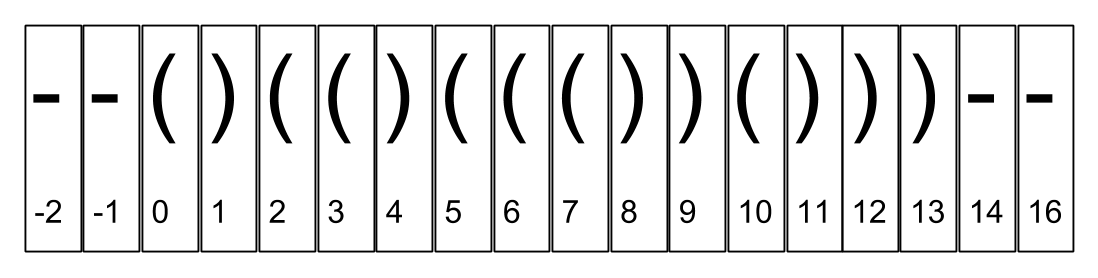
\includegraphics[width=140mm]{Body/figures/ICERtapeLocations.png}
\caption{Tape on which all 148 two-state Turing machines were tested, and the numbering system by which locations along the test tape are identified.}
\label{tapeLocations}
\end{subfigure}

\begin{subfigure}[b]{1.0\textwidth}
\centering
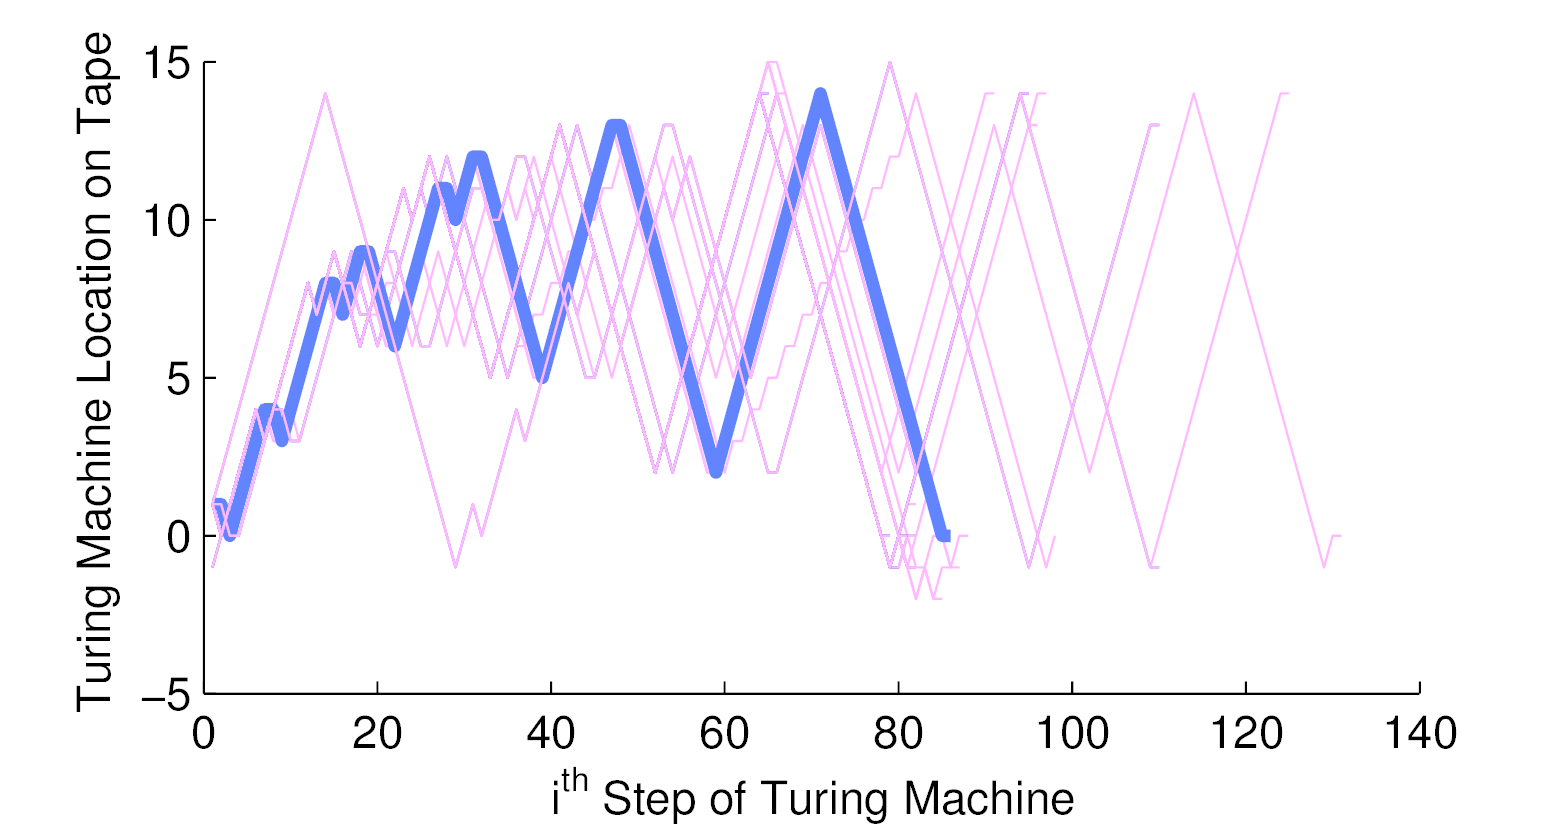
\includegraphics[width=0.85\textwidth]{Body/figures/tmvisualization_InnerParensMatched_allkidsAnno2}
\caption{Strategy A Turing machines: those which paired inner sets of open and closed parentheses, as is standard in mathematical notation. (73 out of 148 Turing machines)}
\label{tapeMoveA}
\end{subfigure}

\begin{subfigure}[b]{1.0\textwidth}
\centering
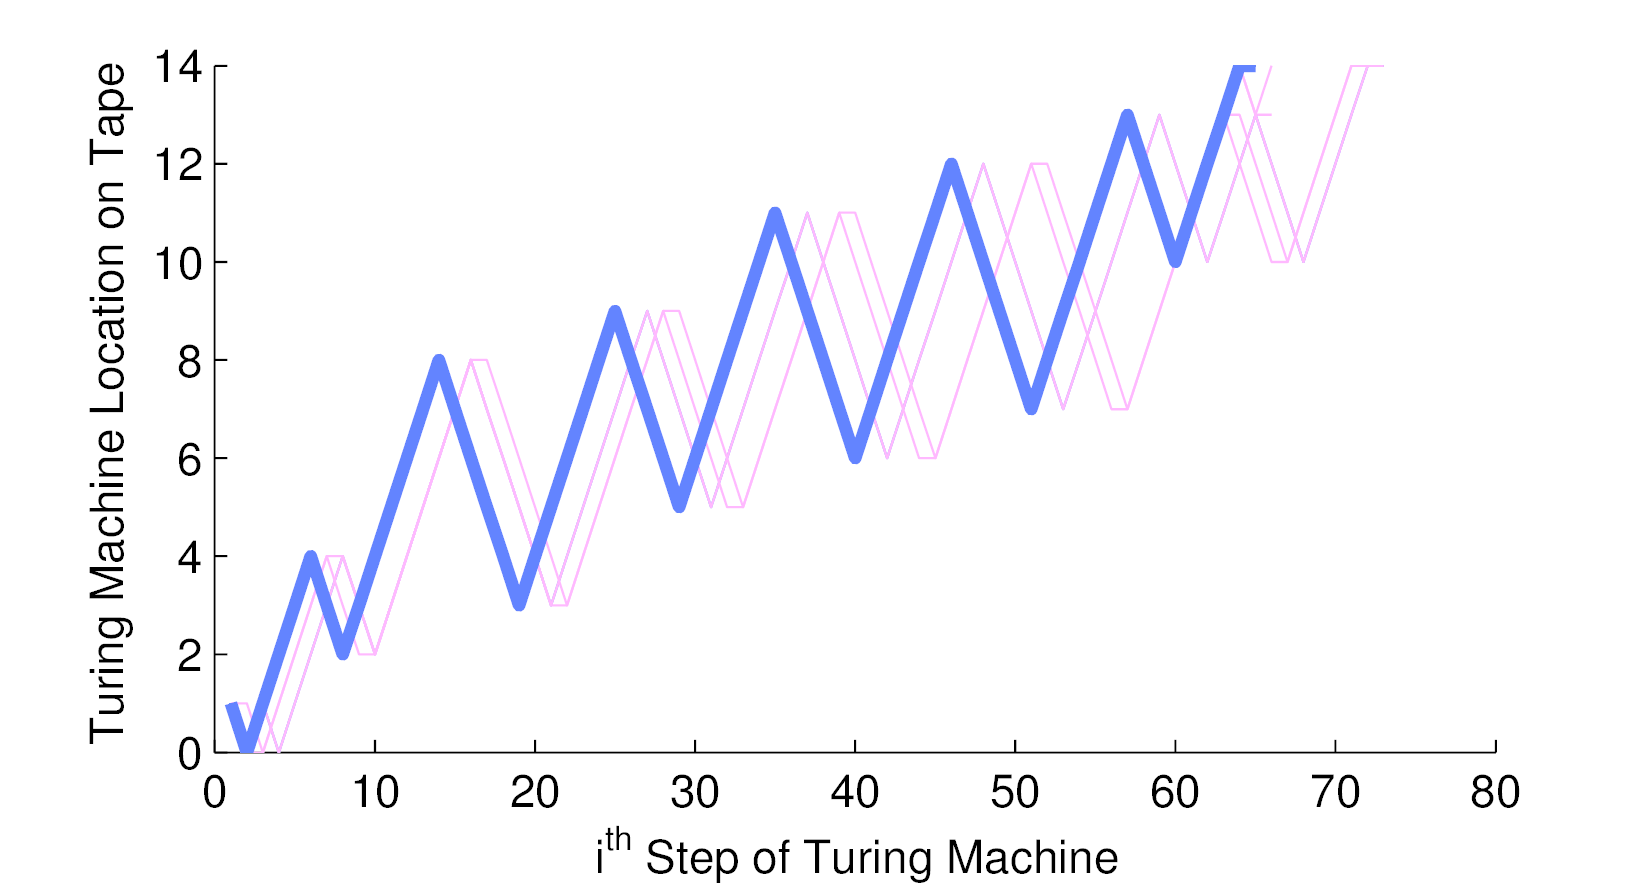
\includegraphics[width=0.85\textwidth]{Body/figures/tmvisualization_NtoNParensMatched_allkidsAnno2}
\caption{Strategy B Turing machines: those which paired the first open with the first closed parenthesis, the second open with the second closed parenthesis, etc. (58 out of 148 Turing machines)}
\label{tapeMoveB}
\end{subfigure}

\caption{The two most common strategies for a two-state Turing machine to determine if a string of parentheses is balanced. Figures \ref{tapeMoveA} and \ref{tapeMoveB} show tape head position over time on the tape illustrated in Fig. \ref{tapeLocations}. The bold trajectories represent particularly clean examples.}
\label{turingFig}
\end{figure*}

The remaining approximately 10\% solutions (not shown) include less common strategies, including at least two that are actually incorrect, i.e., cannot handle arbitrarily deep nesting of parentheses, but are marked as correct because they pass all the test cases in the teacher-designed suite. Many teaching staff members:
\begin{enumerate}
\item were aware of the Turing machine solution they each had found on their own time.
\item not aware that there were two mutually exclusive common solutions. At least one staff member admitted steering students away from solutions they did not recognize, but in retrospect may have indeed been valid solutions.
\item not aware that the test suite was insufficient to determine correctness.
\end{enumerate}

I was able to brief fellow staff members on the space of solutions, both good and bad, in preparation for subsequent semesters and suggested additions to the test tape suite to catch more submissions that were previously erroneously marked as correct.

\section{OverCode}

Analogous to tracking Turing machine movement, my colleague Rishabh Singh and I realized that we could identify meaningful patterns in Python solutions by tracking the values of variables during execution on test cases. He had a pile of student-written Python solutions to the same programming exercise, freshly dumped from the logs of MIT's introductory Python programming course on edX. 

Understanding solution variation is important for providing appropriate feedback to students at scale. The wide variation among these solutions can be a source of pedagogically valuable examples, and can be used to refine the autograder for the exercise by exposing corner cases. We brought in Philip Guo, who contributed variable value-logging code from his Online Python Tutor, and Jeremy Scott, who helped implement the UI, and together, we created and tested OverCode, a system for visualizing and exploring thousands of programming solutions.

OverCode uses both static and dynamic analysis to cluster similar solutions, and lets teachers further filter and cluster solutions based on different criteria. We evaluated OverCode against a non-clustering baseline in a within-subjects study with 24 teaching assistants, and found that the OverCode interface allows teachers to more quickly develop a high-level view of student understanding and misconceptions, and to provide feedback that is relevant to more student solutions.

OverCode addressed the first two of my three frustrations as a teaching assistant:
\begin{enumerate}
\item It canonicalizes students' code so that I can skim their answers as a group or as individuals without first adjusting to each of their variable naming, statement ordering, and style choices.
\item The diversity and distribution of good and bad designs generated by our students is made explicit and explorable. For example, OverCode shows common solutions, which are often reasonable since many students independently arrived at them, and as the user scrolls to less common solutions, solutions can become more convoluted, include unnecessary code, use reasonable alternative Python language keywords and constructs, or solve the problem using teacher-forbidden strategies, e.g., recursively rather than interatively.
\end{enumerate}

\begin{figure}
\centering
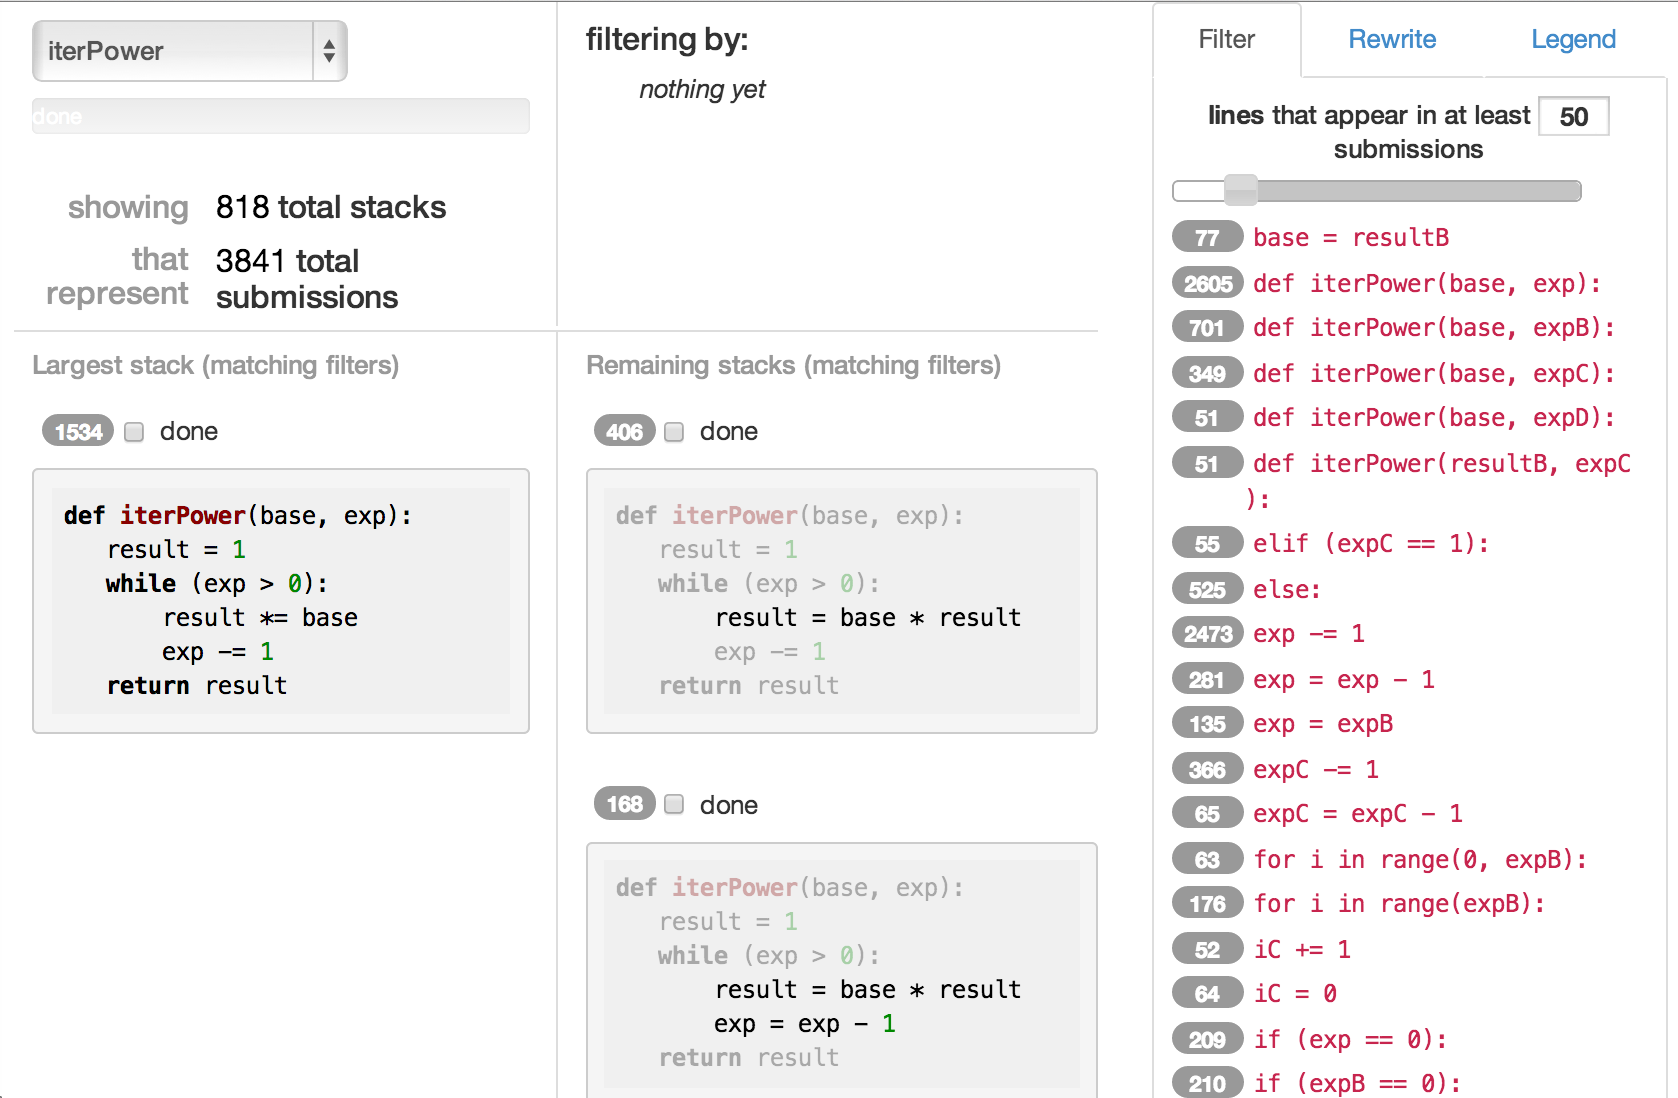
\includegraphics[width=1.0\linewidth]{Body/figures/interfaceScreenShot.png}
\caption{The OverCode user interface. The top left panel shows the number of clusters, called {\it stacks}, and the total number of solutions visualized. The next panel down in the first column shows the largest stack, while the second column shows the remaining stacks. The third column shows the lines of code occurring in the cleaned solutions of the stacks together with their frequencies.}
\label{fullinterface}
\end{figure}


\section{Foobaz}

I approached Ana Bell, the lecturer who served both MIT's residential and online introductory Python programming courses. She found the OverCode interface interesting and hoped to use it, then asked if OverCode could also show her more about students' variable name choices. In a second meeting, her co-teacher, Professor John Guttag, explained that some introductory students mix themselves up by creating names that suggest something other than what the variable contains, e.g., swapping names for the index into an array with the name for the value in the array at that index. It can throw a wrench into their program comprehension process.

Some people undervalue variable names, but they are the most basic form of documentation that helps humans read programs. Donald Knuth compares a good programmer to an essayist who, ``with thesaurus in hand, chooses the names of variables carefully and explains what each variable means'' \cite{literateprogramming}. Without modifying execution, names can express to the human reader the type and purpose of an object, as well as suggest what the kinds of operators used to manipulate it \cite{operands}. Various naming conventions, like Hungarian notation, have evolved to help developers use their freedom wisely. The Google C++ Style Guide authors assert that their most important consistency rules govern naming, which are arbitrary but consistent in order to increase human readability. 

Programmers can develop their own heuristics for good variable names through the experiential learning process of building, debugging, and sharing increasingly large programs with others and their future selves. During informal interviews with programmers in my social network, one professor explained an elaborate set of guidelines that she personally developed and teaches to her students, e.g., all method names must be verbs \cite{doshiconversation}.

In practice, very little time is spent on variable naming in introductory classes. One student-taught month-long introductory Python course offered at MIT spends one lecture on it, and does not systematically assess students' naming choices afterwards. Maybe, with new tools, giving feedback on variable names could become time-efficient and scalable enough to become common place.

Building on top of OverCode and the support of my co-authors Jeremy Scott and Lyla Fischer, I designed and implemented Foobaz, a system that enables time-efficient, scalable, personalized variable name feedback within the context of existing assigned programming exercises. Foobaz distinguishes variables by their behavior in the program, allowing teachers to comment not only on poor names, but also on names that mislead the reader about the variable's role. As shown in Figure \ref{fig:foobaz_teacherview}, the teacher's view is a variable name browser where names are shown along with all the context necessary to judge their quality. Teachers only need to annotate a small number of variable names with qualitative judgements in order to generate personalized formative assessments about variable naming for the majority of their students.

In our first user study, the Foobaz system helped each of 10 teachers give personalized variable name feedback on thousands of student solutions from MIT's edX introductory Python programming course. In the second study, students composed solutions to the same programming assignments and immediately received personalized quizzes composed by the teachers in the previous user study, like the one shown in Figure~\ref{fig:foobaz_studentview}.

Traditional feedback methods, such as hand-grading student code for substance and style, are labor intensive and do not scale. Foobaz addresses feedback at scale for a particular and important aspect of code quality. And, like OverCode, Foobaz addressed the second of my three frustrations as a teaching assistant: making the diversity and distribution of good and bad choices, i.e., variable names, explicit. But what about my last frustration as a teaching assistant, about helping students even get to a correct solution?

\begin{figure*}[p]

\begin{subfigure}[b]{1.0\textwidth}
\centering
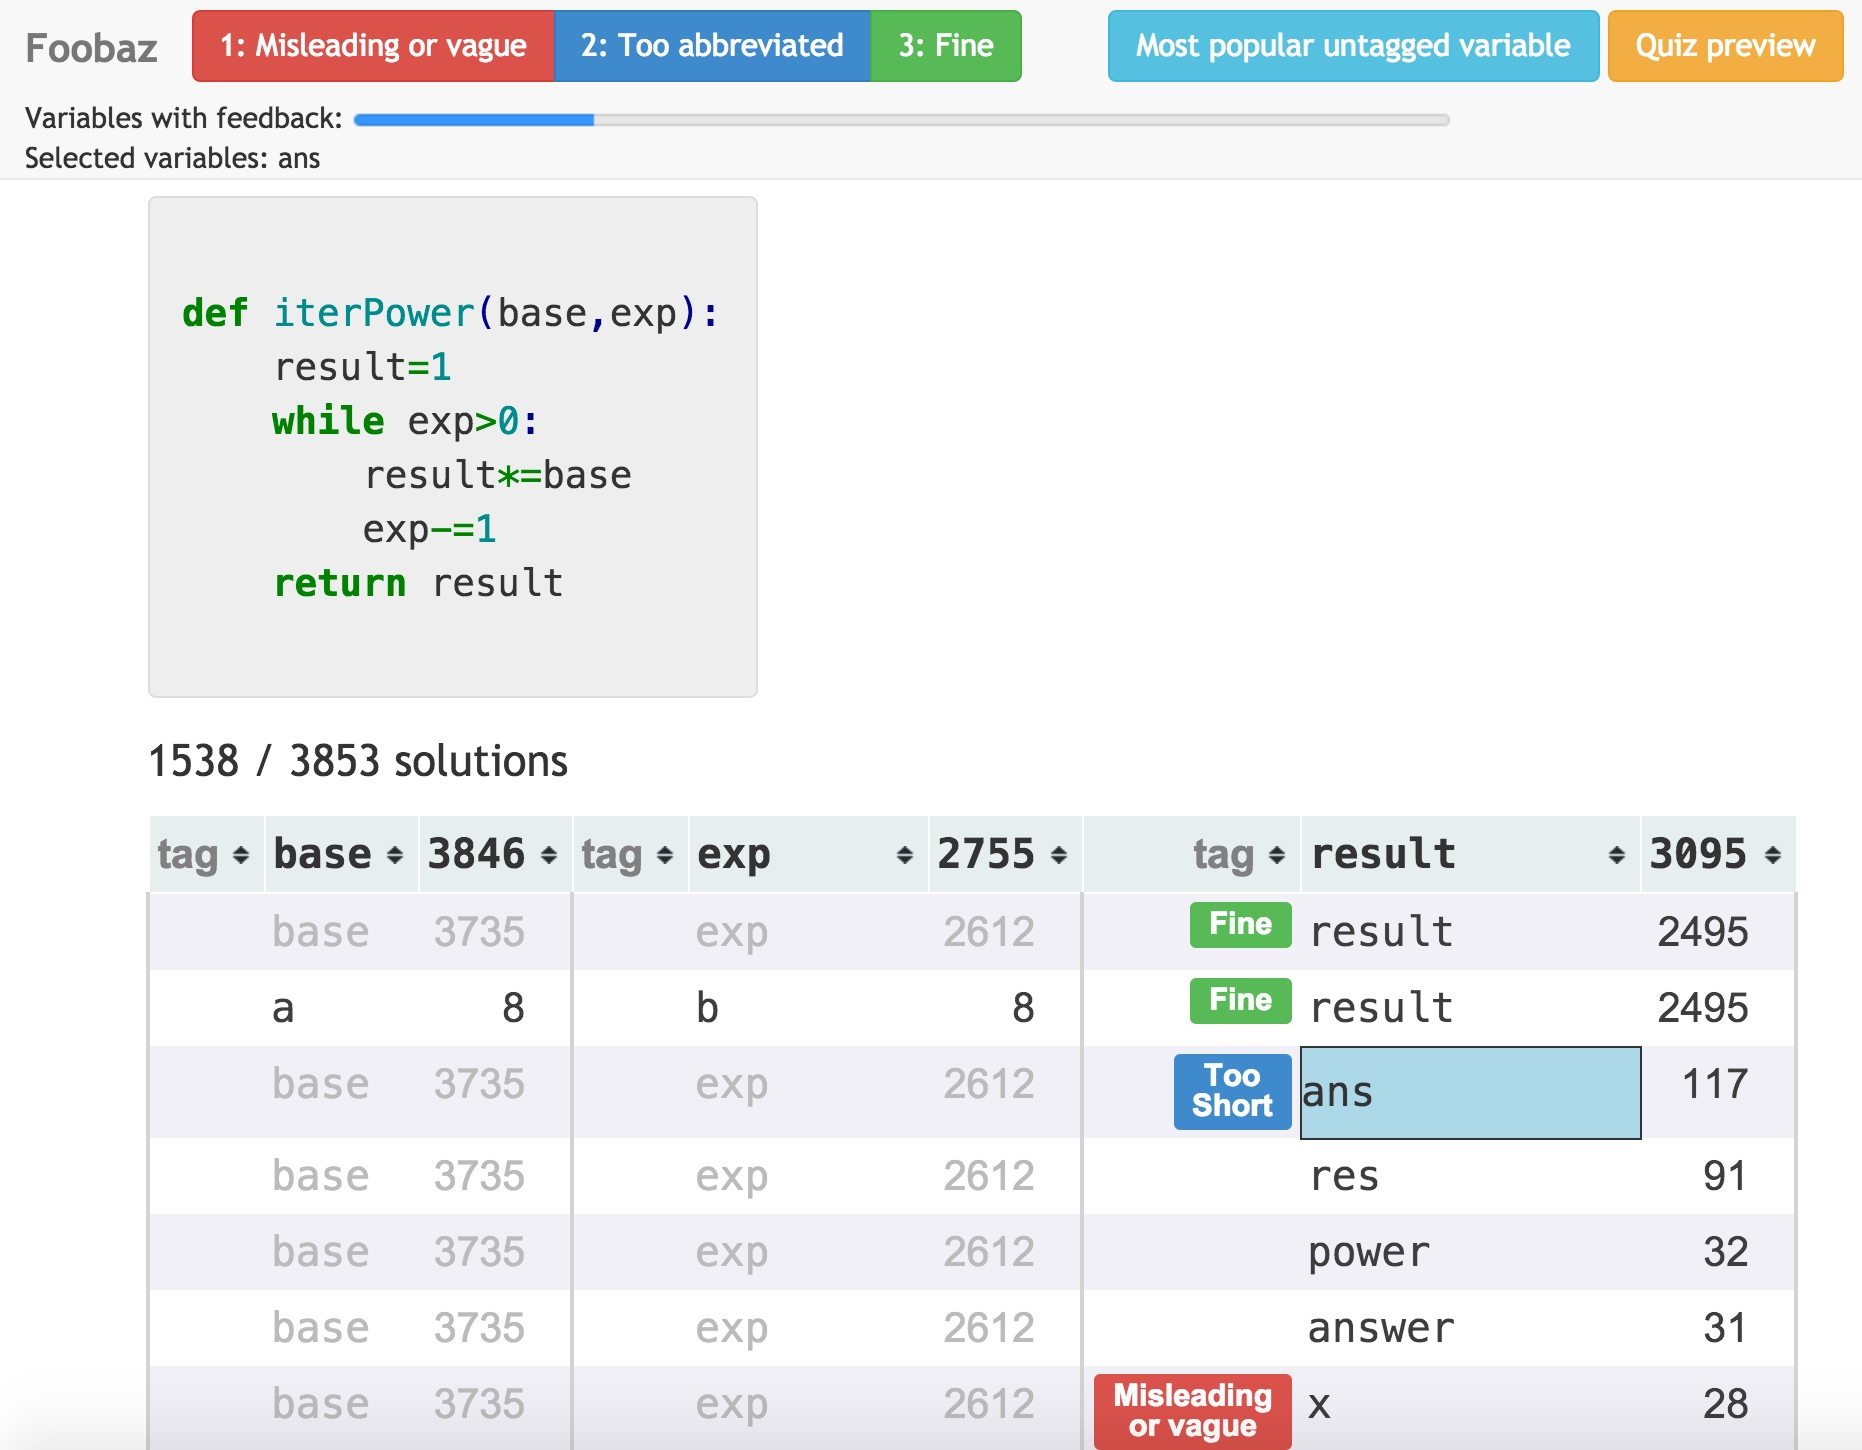
\includegraphics[width=0.75\linewidth]{Body/figures/foobaz/FoobazInitialView4.jpg}
\caption{The Foobaz teacher interface. The teacher is presented with a scrollable list of normalized solutions, each followed by a table of student-chosen variable names. Some names shown here have been labeled by the teacher as ``misleading or vague,'' ``too short,'' or ``fine.''}
\label{fig:foobaz_teacherview}
\end{subfigure}

\begin{subfigure}[b]{1.0\textwidth}
\centering
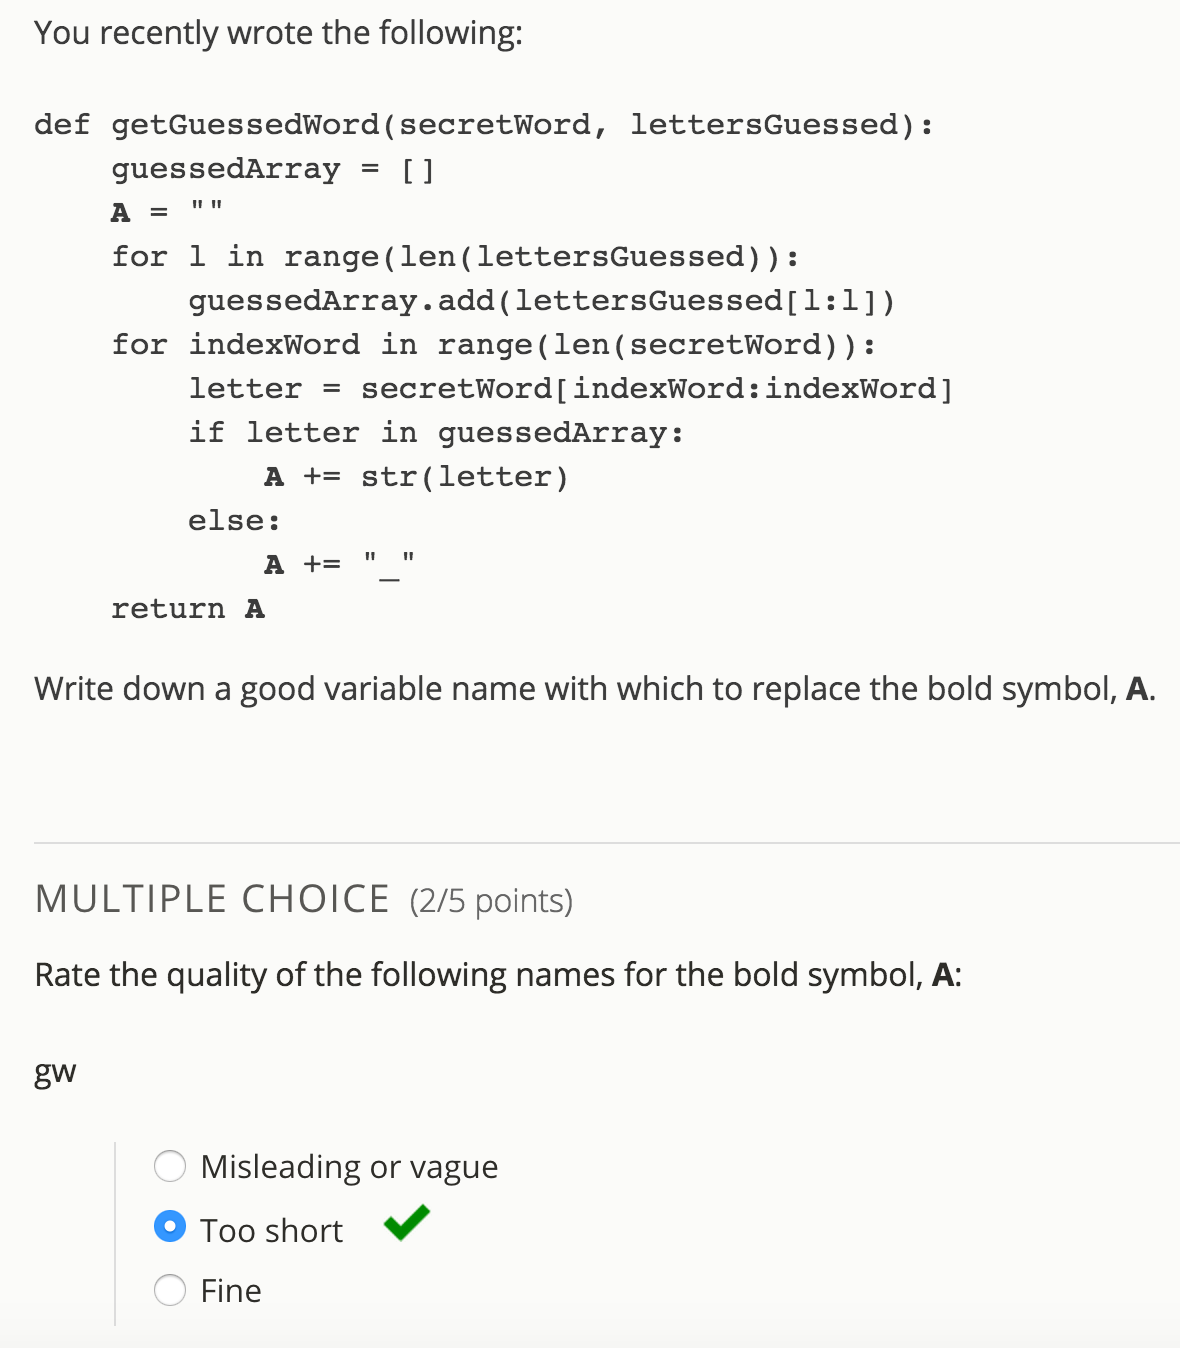
\includegraphics[width=0.4\linewidth]{Body/figures/foobaz/feedbackQuizExample.png}
\caption{A personalized quiz as seen by the student, delivered by an edX-based system maintained by a large university. Students are shown their own code, with a variable name replaced by an arbitrary symbol, followed by variable names for the student to consider and label using the same labels that were available to the teacher. After the student has submitted their own judgments, the teacher’s labels are revealed, along with their explanatory comments.}
\label{fig:foobaz_studentview}
\end{subfigure}

\caption{Snapshots of the Foobaz teacher interface and student variable name quiz}
\end{figure*}
\todo{replace quiz screenshot with system screenshot}


\section{ClassOverflow}

I had built, validated, and published two systems now, all for correct solutions. It is not unreasonable to focus on correct solution in an environment where most students in introductory programming classes can check and check and check their code against teacher-designed test suites until they pass. However, a huge amount of teaching staff time, especially in residential environments, on helping students get to a correct solution.

I recalled yet another stressful moment in the computer lab as a teaching assistant:

    Student A: “I cannot figure out why I’m having this bug.”

    Me: “Oh, I haven’t seen this behavior before. Strange…”

    <We sit together, brainstorming, trying things, debugging, stuck…>

    Student B walks in, overhears us: “Oh, I just had that buggy behavior. Have you considered…?”

    They chatted. Yes, they had separately created the same bug, one after the other. Student B helped Student A debug it. Mystery solved!

By random chance or because I am not a novice, I had not generated that problem in my own code before, but Student B had. I could model good debugging skills, but Student B could be just as, if not more, helpful to Student A in a short amount of time. Student B had earned expertise through experience that I had not.

I felt a mixture of pride at this peer-teaching moment, relief that Student A could move on, and embarrassment that I had not found the bug myself, as the supposed expert in the room.

Personalized support for students is a gold standard in education, but it scales poorly with the number of students. Prior work on \textit{learnersourcing} presented an approach for learners to engage in human computation tasks while trying to learn a new skill. Our key insight is that students, through their own experience struggling with a particular problem, can become experts on the particular optimizations they implement or bugs they resolve. The students can then generate hints for fellow students based on their new expertise. ClassOverflow  uses new workflows to harvest and organize students' collective knowledge and advice for helping fellow novices through design problems in engineering (see Figure \ref{fig:workflow}). ClassOverflow was evaluated in an undergraduate digital hardware design class with hundreds of students. We show that, given our design choices, students can create helpful hints for their peers that augment or even replace teachers' personalized assistance, especially when that assistance is not available.


\begin{figure}
\centering
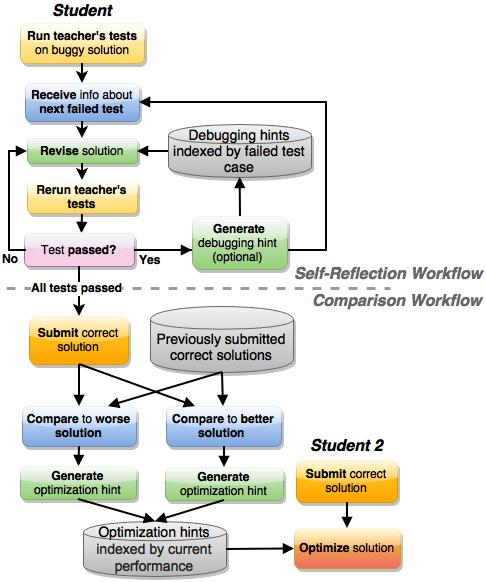
\includegraphics[width=1.0\linewidth]{Body/figures/classoverflow/CombinedWorkflow_CameraReady_FIXED_2.jpg}
\caption{In the \textit{self-reflection} workflow, students generate hints by reflecting on an obstacle they themselves have recently overcome. In the \textit{comparison} workflow, students compare their own solutions to those of other students, generating a hint as a byproduct of explaining how one might get from one solution to the other.}
\label{fig:workflow}
\end{figure}

\section{Extensions of OverCode Clustering}

In order to perform more comprehensive clustering, several extensions of the original OverCode clustering methods have been explored and some have been fully implemented.
GroverCode is an extension of OverCode built to canonicalize and cluster both correct and incorrect solutions. This was also done in the context of hundreds of exam-level solutions instead of thousands of solutions to "finger exercises" and problem set problems. This change in regime was inspired by need-finding interviews with the lecturer who teaches both the online and residential versions of MIT's introductory Python programming class. She was appreciative of the insights OverCode could give her extracted from the thousands of correct solutions submitted by her online students, but the semi-regular pain of hand-grading the hundreds of incorrect solutions submitted by tuition-paying residential students was a more immediate concern. Adapting to the needs of a team of graders grading a smaller number of more complex solutions, many of which were incorrect, required significant changes to the pipeline and interface. The resulting system was deployed to the staff for use during two grading sessions. The results of this field deployment are also promising; the staff welcomes its continued use in future semesters. More preliminary explorations of statistical methods for clustering solutions are also described.


\begin{comment}
\section{Discussion}
Learnersourcing has been a recurring topic at CSCW recently, and these systems show various mechanisms for leveraging learners in large engineering classes. Learners produce many variations of solutions to a problem, running into common and uncommon bugs along the way. Learners can be part of a closed system workflow that prompts them to generate analysis of their own activity and sends it to selected fellow learners as feedback. Alternatively, learners can be pure producers whose activity is analyzed by systems and distilled by teachers into personalized feedback for fellow learners. We would like to demo these systems together, as a suite of learnersourcing systems that allow teachers to turn the challenges of teaching at scale into an opportunity for discussion, self-reflection, peer-teaching, and more learning from examples.
\end{comment}


My thesis statement is: 
\begin{displayquote}
Clustering and visualizing solution variation collected from programming courses can help teachers gain insights into student design choices, detect autograder failures, award partial credit, use targeted learnersourcing to collect hints for other students, and give personalized style feedback at scale.
\end{displayquote}
\todo{make sure targeted learnersourcing is defined}

\section{Terminology}

\todo{Finish defining: solutions, programming exercise/problem, collections of solutions to an exercise....}

Since terminology across research domains can vary, I will define the terms in which I will describe previous research and my own: 
\begin{itemize}
\item A {\it solution} is code that a particular person wrote in response to a prompt or problem description.
\item {\it Solution clusters} represent different patterns of implementation. For example, there may be two distinct solution clusters, both achieving the same input-output behavior but by different means. \todo{better name for this, that respects topic model approach?}
\item A {\it solution path} is a series of code snapshots generated while a person is working toward meeting a particular input-output behavior specification. 
\item The {\it space of student solutions} refers to the aggregation of student-generated solutions and the solution clusters they form.
\item {\it Learnersourcing}... \todo{define, using my own wording if necessary}
\end{itemize}

\section{Contributions}

\todo{add grovercode contributions, turn into prose}The main contributions of this thesis are:
\begin{itemize}
\item A novel visualization that shows similarity and variation among thousands of Python solutions, with cleaned code shown for each variant. 
\item An algorithm that uses the behavior of variables to help cluster Python solutions and generate the cleaned code for each cluster of solutions.
\item Two user studies that show this visualization is useful for giving teachers a birds-eye view of thousands of students' Python solutions.
\item A technique for displaying clusters of Python solutions with only a slice of each cluster exposed, revealing the features that are relevant to the task. In this application, the relevant features are variable names and roles.
\item A workflow for generating personalized active learning exercises, emulating how a teacher might socratically discuss good and bad choices with a student while they review the student's solution together.
\item A working system which implements the above technique and method for datasets from both MOOCs and large residential classes on introductory Python programming.
\item Two lab studies which evaluate both the teachers' and students' experience of the variable name feedback workflow.
\item{A self-reflection learnersourcing workflow in which students generate hints for each other by reflecting on an obstacle they themselves have recently overcome while debugging their solution to a Python or digital design exercise.}
\item{A comparison learnersourcing workflow in which students generate design hints for each other by comparing their own solutions to alternative designs submitted by other students.} 
\item{A deployment of the self-reflection workflow in a 200-student class and a lab study of the comparison workflow with 9 participants. Results from these studies show that personalized hints can be viably learnersourced, and that these hints serve as helpful guides to fellow students encountering the same obstacle or attempting to reach the same goal.}
\end{itemize}

\section{Thesis Overview}

Chapter \ref{chapter:relatedwork} summarizes prior and contemporary relevant research on systems that support programming education. It also briefly explains theories from the learning sciences and psychology literature that influenced or support the pedagogical value of the design choices made within this thesis.

The four chapters that follow describe, in detail, the four systems developed, as well as their evaluation on archived data or in the field.

\begin{itemize}
\item OverCode (Chapter \ref{chapter:overcode}) visualizes thousands of programming solutions using static and dynamic analysis to cluster similar solutions. It lets teachers quickly develop a high-level view of student understanding and misconceptions and provide feedback that is relevant to many student solutions. 

\item Foobaz (Chapter \ref{chapter:foobaz}) clusters variables in student programs by their names and behavior so that teachers can give feedback on variable naming. Rather than requiring the teacher to comment on thousands of students individually, Foobaz generates personalized quizzes that help students evaluate their own names by comparing them with good and bad names from other students. 

\item ClassOverflow (Chapter \ref{chapter:classoverflow}) collects and organizes solution hints indexed by the autograder test that failed or a performance characteristic like size or speed. It helps students reflect on their debugging or optimization process, generates hints that can help other students with the same problem, and could potentially bootstrap an intelligent tutor tailored to the problem.

\item OverCode Extensions (Chapter \ref{chapter:grovercode}) describes (1) GroverCode, an extension to OverCode optimized for processing and displaying incorrect as well as correct student submissions and (2) clustering and mixture modeling algorithms applied to the OverCode pipeline's output for additional insight into patterns within student solutions. %The GroverCode user interface is optimized and deployed in the field for teachers awarding partial credit to each of the hundreds of students who submitted programs in computer-based quizzes and final exams for the residential Python-based introductory programming (6.0001) and data science (6.0002) courses at MIT.
\end{itemize}

Chapter \ref{chapter:discussion} discusses the design lessons that apply to the entire collection of systems in this thesis. Chapter \ref{chapter:futurework} outlines avenues of future work this thesis work, in combination with the complementary work of others in this space, paves the way for.



\begin{comment}"one-on-one tutoring promotes both greater student learning and increased student motivation to learn compared with traditional, formal classroom teaching and learning settings" --http://www.ncbi.nlm.nih.gov/pmc/articles/PMC3292071/ \end{comment}


\begin{comment}

Dead kittens:

In introductory programming and digital circuit design education, this thesis aims to change the traditional curve in the quality of education as a function of class size from monotonically decreasing to a U-shape. As a proxy for measuring learning outcomes, the systems developed in this thesis empower old or entirely new rapid, personalized feedback modes similar to those delivered in a one-on-one teaching relationship but enabled by the scale of students composing solutions to class exercises.

By second grade, children should be able to write simple, coherent stories \cite{http://www.webmd.com/parenting/features/when-should-kids-learn-read-write-math}. 

When I was much younger, my dad taught me about vacuum tubes. With few modifications, tubes can serve as amplifiers, switches, or displays. ``Tube: The Invention of Television'' tells the dramatic history behind the invention and commericialization of the first televisions, which were built with cathode ray tubes. At critical parts of the story, he'd ask, e.g., ``How you would change the intensity of the electron beam hitting the screen?'' just before the authors were about to reveal how the inventors would get past their next technological hurdle.

Sometimes, I had no idea how to answer. Sometimes, I came up with something similar to what the inventors came up with. And sometimes, because I was not biased by the actual scientific literature that the inventors were immersed in, I came up with something very different, but possibly also effective. 

The systems in this thesis help teachers take advantage of the massive collections of solutions, enabling either (1) the same teaching practices that were previously only tractable in smaller courses or (2) new practices that are only possible when a massive collection of student solutions are available.

This thesis describes several systems designed to (1)  (2) (3) amplify teachers' actions, by enabling them to compose and deliver personalized feedback to more students while expending minimal additional effort. 

Despite recent advances in artificial intelligence, human and computer intelligence remain largely complementary. Humans can compose new questions and handle novel answers, while computers can perform prescribed analyses of thousands of student answers orders of magnitude faster than humans. 

Ways of delivering the rapid, personalized feedback that  commonly accepted practices of good teaching d

As enrollment in programming courses grows, some teaching practices and systems may become prohibitively expensive or arduous to use.

This thesis documents several novel tools I developed for helping hundreds or thousands of students learn how to program. The demand for programming education is growing rapidly, and this thesis treats the volume of students in programming classes not as a problem, but as an opportunity. It begins with the story of how I learned to program, and ends with a description of new tools for teachers and students engaged in the hard work of transferring the knowledge and practice of programming from one generation to the next.

At heart, I'm an electrical engineer, and it has informed my approach through-out. To me, a class of students is a system I want closed-loop control over: with the control policy of an experienced teacher and knowledge of the state of the system--my hundreds or thousands of students--I can better steer it to my intended destination of knowledge and skills.

I similarly think of solutions as systems that turn inputs into outputs, sometimes in the same way, sometimes in different ways.
\end{comment}

\begin{comment}Dead kitten: since the first CS degrees were awarded in the late 1960s
\footnote{Some CS departments are considering or already implementing course enrollment limits, which may disproportionately affect underrepresented students \cite{personalconversationwithjasonchuang}.}
Enrollment in computer science, including programming classes, has been growing. We are now experiencing a third boom in student interest \cite{csBoom}.
\end{comment} 

%% This is an example first chapter.  You should put chapter/appendix that you
%% write into a separate file, and add a line \include{yourfilename} to
%% main.tex, where `yourfilename.tex' is the name of the chapter/appendix file.
%% You can process specific files by typing their names in at the 
%% \files=
%% prompt when you run the file main.tex through LaTeX.
\chapter{Related Work}\label{chapter:relatedwork}

Systems that help students in massive programming courses may build on work from any or all the following related fields: program analysis, program synthesis, crowd workflows, user-interface design, machine learning, and learning science. First, I present prior work and theories of how people learn that later inspired key design decisions. I then clarify how this thesis work is novel by describing related work that achieves similar goals or uses similar methods.

Computers' potential as teaching aids was recognized soon after their development; not long after it was physically possible to bring a computer into the classroom, they were used as vehicles for education \cite{computersInEdu}. Modern computer-aided instruction includes intelligent tutoring systems, automated tutorials, power-grading systems, and massive open online course platforms. 

\todo{add cody! (see ICER submission)}
\todo{look into PHOG and other interesting work here: http://www.srl.inf.ethz.ch/spas.php http://www.srl.inf.ethz.ch/raychev.php and "Predicting Program Properties from “Big Code” http://www.srl.inf.ethz.ch/papers/jsnice15.pdf and "Code Completion with Statistical Language Models" http://www.srl.inf.ethz.ch/papers/pldi14-statistical.pdf}

\todo{Analyzing Engineering Design through the Lens of Computation
Authors
Marcelo Worsley, Paulo Blikstein}

\todo{Teaching composition quality at scale: human judgment in the age of autograders
Authors
John DeNero, Stephen Martinis}

\todo{Problems Before Solutions: Automated Problem Clarification at Scale
Authors
Soumya Basu, Albert Wu, Brian Hou, John DeNero}

\todo{CS10K Teachers by 2017?: Try CS1K+ students NOW! Coping with the Largest CS1 Courses in History
Authors
Daniel D Garcia, Jennifer Campbell, John DeNero, Mary Lou Dorf, Stuart Reges}

\todo{Fuzz Testing Projects in Massive Courses
Authors
Sumukh Sridhara, Brian Hou, Jeffrey Lu, John DeNero}

\todo{https://computinged.wordpress.com/2012/12/14/research-questions-on-moocs-whos-talking-whos-completing-and-wheres-the-teaching/}

\todo{https://computinged.wordpress.com/2012/08/14/daphne-kollers-ted-talk-whats-new-about-moocs/

The Relative Effectiveness of Human Tutoring,
Intelligent Tutoring Systems, and Other Tutoring
Systems
KURT VanLEHN $http://www.public.asu.edu/~kvanlehn/Stringent/PDF/EffectivenessOfTutoring_Vanlehn.pdf$}

\todo{cite Techniques for Plan Recognition
SANDRA CARBERRY for solution path mining, but I did not do that...}
\todo{Automated Feedback Generation for

Introductory Programming Assignments

Rishabh Singh}

\todo{Learning Design Patterns
with Bayesian Grammar Induction
Jerry O. Talton et al. http://graphics.stanford.edu/~lfyg/gi.pdf}

\todo{http://cs.stanford.edu/people/sharmar/pubs/ddec.pdf Data-driven equivalence checking}

\todo{Mining Source Code Repositories at Massive Scale
using Language Modeling
Miltiadis Allamanis, Charles Sutton}

\todo{Student coding styles as predictors of help-seeking behavior
Authors
Engin Bumbacher, Alfredo Sandes, Amit Deutsch, Paulo Blikstein}

\todo{see library on Google Scholar, Vineet's review of literature}

\todo{Programming Pathways: A Technique for Analyzing Novice Programmers’ Learning Trajectories
Authors
Marcelo Worsley, Paulo Blikstein}

\todo{Educational data mining and learning analytics: Applications to constructionist research
Authors
Matthew Berland, Ryan S Baker, Paulo Blikstein}

\todo{cite WebZeitGeist}

\todo{Programming pluralism: Using learning analytics to detect patterns in the learning of computer programming
Authors
Paulo Blikstein, Marcelo Worsley, Chris Piech, Mehran Sahami, Steven Cooper, Daphne Koller}

\todo{cite Using learning analytics to assess students' behavior in open-ended programming tasks
Authors
Paulo Blikstein}

\todo{Modeling how students learn to program
Authors
Chris Piech, Mehran Sahami, Daphne Koller, Steve Cooper, Paulo Blikstein}

\todo{see Related Work folder in Google Drive and Question Independent Grading using Machine Learning:

The Case of Computer Program Grading

Gursimran Singh

Shashank Srikant

Varun Aggarwal}

\todo{add The Sweep: Essential Examples for In-Flow Peer Review by
JG Politz, JM Collard, A Guha, K Fisler, S Krishnamurthi and In-flow peer-review of tests in test-first programming
Authors
Joe Gibbs Politz, Shriram Krishnamurthi, Kathi Fisler and In-Flow Peer Review
Authors
Dave Clarke, Tony Clear, Kathi Fisler, Matthias Hauswirth, Shriram Krishnamurthi, Joe Gibbs Politz, Ville Tirronen, Tobias Wrigstad and CaptainTeach: a platform for in-flow peer review of programming assignments
Authors
Joe Gibbs Politz, Shriram Krishnamurthi, Kathi Fisler and CaptainTeach: Multi-stage, in-flow peer review for programming assignments
Authors
Joe Gibbs Politz, Daniel Patterson, Shriram Krishnamurthi, Kathi Fisler}

\todo{add this to related work https://computinged.wordpress.com/2016/05/16/implementing-design-studio-pedagogy-with-an-augmented-reality-cs-classroom/}

\section{Learning from Variation}

\begin{comment}
Marton et al.'s variation theory \cite{Marton13} holds that in order to learn something, one must see examples that vary along particular dimensions: ``contrast,'' as in pairing it with something it is not; ``generalization,'' as in presenting multiple instances of the object or concept to be learned, varying only that which is irrelevant; ``separation,'' as in presenting multiple instances of the object or concept, varying only that which can vary internally without changing the object or concept into something else; and ``fusion,'' as in seeing multiple examples in which previously analytically separated aspects must be processed together to recognize the object or concept. The aspects which are related to these dimensions of variation and therefore define the object or concept are called ``critical features.''
\end{comment}

\subsection{Variation Theory}
Marton's Variation Theory, as summarized by Suhonen et al. \cite{suhonen}, is defined by the dimensions of variation necessary to fully communicate a concept to a student: \emph{contrast} (``in order to experience something, a person must experience something else to compare it with''); \emph{generalization}, or the ways something can vary without becoming something else; \emph{separation}, or looking at the variation only across specific features; and \emph{fusion}, where multiple critical aspects of the concept are varied simultaneously. In other words, variation reveals which aspects of a phenomenon are superficial/irrelevant and which are innate/critical to its definition \cite{Leung}. These aspects that define the object or concept are called ``critical features.'' The Variation Theory is a framework that now guides the design of some critical reading exercises \cite{Tong} and exercises for novice programmers \cite{eckerdal}. 

Given Marton et al.'s rubric for effective patterns of variation, and the identification of ``critical features,'' one can discern between more or less theoretically effective examples of the object or concept given to a student to learn. On this basis, Luxton-Reilly et al. \cite{Luxton13} suggest that identifying distinct clusters of solutions can help instructors select appropriate examples of code for helping students learn. They also suggest that it is helpful for teachers' own understanding and quality of feedback and guidance. Facilitating the discovery or identification of critical features, which are possibly both teacher-specific and task-specific, is a major challenge I will address in this thesis. 

Other pedagogical strategies that involve comparing and contrasting examples have also been shown to have learning benefits. The pedagogical method of comparing and contrasting ways of approaching a solution has now been validated in the literature of mathematics education research \cite{Star07}, cognitive science \cite{loewenstein2003analogical,kurtz01learning,telling}, and computing education research \cite{Suhonen08, PatitsasICER13}. Peer reviews and assessments, surveyed in \cite{peerReview98}, are yet another opportunity for students to learn from compare and contrast.

\subsection{Synthesizing Knowledge Across Sources and Modalities}

The synthesis of understanding derived from multiple sources is critical to journalism and humanities scholarship and in technical fields, like mathematics.

\subsubsection{Humanities Scholarship and Journalistic Analysis}  
Wineburg \cite{wineburg} shows how students of history come to their understanding of complex events. One important behavior is the students' use of multiple simultaneous documents to understand context. Wineburg finds that ``\ldots context is everything \ldots who wrote something; what their political view is; what the situation in the world is at that moment \ldots you need to see the situation from many points-of-view \ldots''

Software has recently been built to help scholars and journalists analyze and synthesize knowledge across sources. For example, the AP's Overview Project is an example of software designed to help journalists analyze thousands of documents. Similarly, WordSeer \cite{wordseer} allows scholars in the humanities to make sense of a corpus of relevant texts by providing the ability to look at multiple sources and do textual analysis of the content. Crowdlines \cite{luther} employed crowd-sourcing to help people learn and synthesize information from diverse online sources. Since humans are skilled at evaluating high-level structure and making connections between sources, crowdworkers created outlines for important topics that included diverse perspectives from multiple document sources. 

Shahaf et al. \cite{shahaf} created algorithms for ``information cartography,'' algorithmically sub-sampling large collections of documents on a common topic and laying them out as a 2-D map of interrelated documents for users to explore and read. This technique has been applied to scholarly publications and news articles on complex current events, such as the European debt crisis or the Israeli-Palestinian conflict. These domains contain interrelated parallel story-lines that evolve and intersect over time, and are represented as such in the resulting ‘Metro Maps’ of information.

\subsubsection{Science, Technology, Engineering and Math (STEM)} 
The simple question, ``What machine learning books are accessible and appropriate for my high school-aged daughter?'' recently kicked off a very lively discussion on a corporate engineering mailing list. It is a question that humans with a model of the learner, e.g., high school student, and the subject matter, e.g., machine learning, can answer well. Jardine \cite{jardine} generated reading lists specifically for novices hoping to become experts in a particular area, using a personalized pagerank function and Latent Topic Models. 

Educational psychologists have found that multiple explanations within and across multiple modalities can help students learn mathematical problem solving. Both Tabachneck et al. \cite{Tabachneck} and Cox and Brna \cite{cox} found that students fared better at problem solving when using multiple strategies and/or representations, such as diagrams, written algebra, tables, and natural language. Ainsworth points out that giving students an opportunity to consider different representations may help them overcome the weaknesses of any particular representation.

This is also supported by authors of Metacademy.com, a popular online resource for teaching yourself machine learning: ``A good general piece of advice is to consult multiple resources. Different textbooks or courses will explain something from a different perspective \ldots [O]ften when reading one, you get an ‘aha!’ moment for something which didn't make sense in the other. Unfortunately, this option might not be practical unless you have access to a university library.'' \cite{metacademy}

\subsection{User Interface Design}
Tufte pioneered a layout technique called ``small multiples,'' designed to help viewers make rapid decisions about a wide array of items or variables: ``Small multiple designs \ldots answer directly by visually enforcing \ldots the differences among objects, \ldots the scope of alternatives.'' %We took inspiration from both of these layouts when designing the flowing grid layout for DocMatrix. 

%The common term sidebar was inspired by Hearst's faceted browsing \cite{facets}. But rather than display facets derived from metadata about each document, we extracted the common terms from a source closer to the content of the documents themselves: the tables of contents. Clicking on any of the terms in this list exposes the tables of contents, with relevant chapter titles highlighted; the actual terms contained in the tables of contents are the key to this ontological alignment.

Grokker is a document-clustering visualization system, with small popup windows to read texts in parallel \cite{slaney}. Unlike DocMatrix, Grokker's primary representation of a corpus of documents is as clusters of dots, but the study design and results are still relevant here. The task for Grokker readers was to quickly browse a large document collection, and then answer a set of questions to test their understanding. A key finding of this study was that small details of document viewability and the amount of time it took the participants to access content dramatically affected how much they understood about the domain.  In other words, small changes in the amount of time to switch between related documents was an important variable.  


\section{Methods for Analyzing Solutions}

While the methods described in this section all analyze solutions written in code, either as individuals or as a collection, some focus on supervised classification of solutions using pre-defined schemas and some focus on unsupervised clustering of code within collections; and some focus on explicitly identifying variation.

\subsection{Methods for Supervised Classification of Solutions}

Taherkhani and collaborators have developed several algorithm recognition methods. Two methods feature prominently in their work: (1) a method that creates a feature vector for the \emph{predefined target solution} based on roles of variables, beacons, and various other software metrics and (2) a method that scans solutions for \emph{predefined schemas} that are associated with algorithms of interest. In \cite{taherkhani13}, Taherkhani et al. have combined the two approaches into a more robust version which only compares software metrics and beacons on the code that have the same schema. While the software metrics used in these approaches are relevant to my thesis, the use of predefined schemas and target solutions is distinct from my approach of purely mining student solutions.

\subsection{Methods for Unsupervised Clustering of Code}

Unsupervised clustering encompasses everything from identifying plagiarism within a collection of solutions submitted by different people to loosely grouping solutions with similar approaches to solving a problem.

\subsubsection{Clone Detection}
There are multiple types of clones. The simplest clone is an exact copy. A parameter-substituted clone only differs from its copy by the values of identifiers and literals. A structure-substituted clone is a copy with something new swapped in for an entire subtree of the syntax tree. This is of particular interest to teachers looking for evidence of plagiarism within or across class offerings and for software engineers performing re-factoring who want to make their code more compliant with the DRY ("Do Not Repeat Yourself") principle of software development.

\citet{tiarks2011extended} does... \todo{expand on what I said earlier: The most powerful algorithm recognition methods can identify clones that are modified beyond just structural substitutions...}

A popular plaigerism detection algorithm, MOSS, uses \todo{winnowed?} document fingerprinting by \citet{schleimer2003winnowing}. A fingerprint is constructed by computing hashes for all $n$-grams in a document (for some chosen $n$). Similar code will contain similar fingerprint components. \todo{it also does parameter substitution, right? and what's this winnowing business? did document fingerprinting exist before this citation?}

%These latter two types of clones are difficult to identify even with current state-of-the-art techniques \cite{taherkhani12, taherkhani13}. 

\subsection{Methods for Describing Solution Variation}

\begin{comment}
Braun and Clarke \cite{thematic06} argue that its application to qualitative data outside psychological research is justified. It is in direct contrast to methods in which a hypothesis or theory is first declared, and then evidence for and against it is gathered from the data. 
\end{comment}

\citet{Luxton13} used thematic analysis to capture the variation between correct solutions in their dataset. Thematic analysis comes out of the field of psychology as a way to build theory from observing patterns in organic, free-form statements from subjects, or, in this case, submissions for coding assignments. They aimed to discover the kinds and degree of variation between student-generated solutions that fulfilled the specifications of short introductory Java programming exercises. By thematic analysis of student submissions, the authors generated a taxonomy that captured the variation between correct solutions in their dataset. They then created an Eclipse plug-in for classifying new code examples based on their taxonomy. 

\section{Methods for Analyzing Paths to Solutions}

Using automated classification methods, \citet{Piech} found distinct development paths students take to achieve working solutions that fulfilled the specifications of short introductory programming exercises in Java. Students' incremental paths were classified by pipeline that included milestone discovery, Hidden Markov Modeling of the students' process, and clustering of solution paths. These identified paths are visualized as finite state machine transition diagrams. The evaluation focused on predicting midterm exam grades and detecting milestone difficulty.

\citet{sudol12} also classify and map out distinct paths to solutions to introductory programming exercises. After using a Markov Model to generate a ``problem state graph,'' the authors applied their Probabilistic Distance to Solution (PDS) metric to the graph to estimate the number of states between an observed program model and the model of a correct solution.

Kiesmueller et al. \cite{Kiesmueller} attempted to recognize strategies at a very high level, which are not specific to the challenge at hand. Example high-level problem-independent strategies were a top-down or bottom-up programming style. Helminen et al. \cite{ICERHelminen} introduced novel interactive graphs for examining the problem solving process of students working on small programming-like problems. However, problems with multiple solutions were outside the scope of their investigation.

%\section{Introduction}
\section{Thesis Proposal}

%I partitioned the related work based on method of discovering the space of solutions and existing structures within learning environments that this knowledge could enhance. The specific domain to which these methods and interventions are applied is noted as each reference is discussed. 

%The work highlighted in the first section below addresses the feasibility and current state-of-the-art in classifying student solutions and solution paths, using machine learning algorithms and visualization methods. The second section highlights work from the Computer Science Education community on the relevance of solution space knowledge to various methods used within learning environments. %The final subsection surveys the existing domains in which these methods have been applied, specifically concerning the type and scale of programming challenges.

Since terminology across research domains can vary, I will define the terms in which I will describe previous research and my own: 
\begin{itemize}
\item A solution is code that a particular person wrote in response to a prompt or problem description.
\item Solution clusters represent different patterns of implementation. For example, there may be two distinct solution clusters, both achieving the same input-output behavior but by different means. 
\item A solution path is a series of code snapshots generated while a person is working toward meeting a particular input-output behavior specification. 
\item The ``space of student solutions'' refers to the aggregation of student-generated solutions and the solution clusters they form.
\end{itemize}

\subsection{Comparing and Contrasting Examples}


Marton et al.'s variation theory \cite{Marton13} holds that in order to learn something, one must see examples that vary along particular dimensions: ``contrast,'' as in pairing it with something it is not; ``generalization,'' as in presenting multiple instances of the object or concept to be learned, varying only that which is irrelevant; ``separation,'' as in presenting multiple instances of the object or concept, varying only that which can vary internally without changing the object or concept into something else; and ``fusion,'' as in seeing multiple examples in which previously analytically separated aspects must be processed together to recognize the object or concept. The aspects which are related to these dimensions of variation and therefore define the object or concept are called ``critical features.''

Peer reviews and assessments, surveyed in \cite{peerReview98}, are one of the existing pedagogies in which teachers ask students to compare and constrast examples. The pedagogical method of comparing and contrasting ways of approaching a solution has now been validated in the literature of mathematics education research \cite{Star07}, cognitive science \cite{loewenstein2003analogical,kurtz01learning,telling}, and computing education research \cite{Suhonen08, PatitsasICER13}.

Given Marton et al.'s rubric for effective patterns of variation, and the identification of ``critical features,'' one can discern between more or less theoretically effective examples of the object or concept given to a student to learn. On this basis, Luxton-Reilly et al. \cite{Luxton13} suggest that identifying distinct clusters of solutions can help instructors select appropriate examples of code for teaching purposes. 

While this research has focused on the effects of multiple, varying examples on student learning, it is also, as suggested by Luxton-Reilly et al. \cite{Luxton13}, helpful for teachers' own understanding and quality of feedback and guidance. Facilitating the discovery or identification of critical features, which are possibly both teacher-specific and task-specific, is a major challenge I will address in this thesis.

\subsection{Feature Engineering}

In order to discover or identify critical features, it is necessary to generate a set of candidate features. A variety of methods have been employed in the literature to select or engineer features, but those which I describe here are focused on features that humans can perceive by looking at the actual code submission.

\subsubsection{Abstract Syntax Trees, Dependency Graphs, and Control Flow Graphs}

Aggarwal et al. \cite{aggarwalprinciples} address the critical nature of feature engineering in the context of machine-learning-based automated grading. The grading rubric is based on the authors' understanding of how humans perceive and assess programs. They describe how humans first look for certain ``signature features,'' such as certain control structures, dependencies, and keywords. If the necessary features are in place, then more fine-grained assessment can be made. Are the correct structures used, and are statements ordered properly? This increasingly fine-grained assessment can continue on, to include terminating conditions and dependencies between data structures, until the human is satisfied. 

Aggarwal et al. suggest extracting these features from a code submission's Abstract Syntax Tree (AST), Control Flow Graph, Data Dependence Graph, and/or Program Dependence Graph. The authors assert that these graphs will be helpful even if the code represents only a partial solution. Note that these features are targeted at labeling each solution with a numerical score based on correctness, not on disguishing between equally correct solutions representing different approaches to a problem.

%, human considerations are weighed heavily in their feature design.

\subsubsection{Thematic Analysis}

Instead of grading submissions based on a rubric of human acceptability and correctness, Luxton-Reilly et al. \cite{Luxton13} used thematic analysis to capture the variation between correct solutions in their dataset. Thematic analysis comes out of the field of psychology as a way to build theory from observing patterns in organic, free-form statements from subjects, or, in this case, submissions for coding assignments. Braun and Clarke \cite{thematic06} argue that its application to qualitative data outside psychological research is justified. It is in direct contrast to methods in which a hypothesis or theory is first declared, and then evidence for and against it is gathered from the data. 

Luxton-Reilly et al. \cite{Luxton13} aim to discover the kinds and degree of variation between student-generated solutions that fulfilled the specifications of short introductory Java programming exercises. By thematic analysis of student submissions, the authors generated a taxonomy that captures the variation between correct solutions in their dataset. They then created an Eclipse plug-in for classifying new code examples based on their taxonomy. 

\subsubsection{Compiler Concepts}

Some of the Java exercises in the corpus studied by Luxton-Reilly et al. \cite{Luxton13} were as simple as writing a function which takes two integers and returns their sum. Within these simple tasks, variation was still found in the way students used parentheses, declared and initialized variables, and made assignments. In order to use established, non-ambiguous terms for their observations, Luxton-Reilly et al. reference compiler concepts, such as tokens, classes of tokens, and control flow graphs. 

They labeled types of variations as structural, syntactic, or relating to presentation. The control flow graphs represent structural variation. The nodes of control flow graphs are blocks of code that have a single entry point, single exit point, and no internal branching. The flow between blocks of code is represented by the edges connecting the control graph nodes. If the control graph (structure) of two solutions is the same, then the syntactic variation within those blocks of code are compared by looking at the sequence of token classes. Presentation-based variation, such as variable names and spacing, is only examined when two solutions are structurally and syntactically the same.

Luxton-Reilly et al.'s Eclipse plugin takes as input a collection of Java source files and creates a library of structurally unique Java code, which becomes the categories of files. On their corpus, they found a small number of highly populated categories, which did not always line up with the category of the instructor's implementation.

\subsubsection{Adding Input-Output Behavior}

Huang et al. \cite{MOOCshop} considered tens of thousands of solutions submitted to Stanford's Fall 2011 Machine Learning MOOC, and identified clusters of solutions based on measures of syntactic but also functional similarity. The syntactic similarity was the edit distance between solutions' ASTs, using the tree edit distance function described in Shasha et al. \cite{shasha1994exact}. Code submissions were also grouped by their success or failure on a battery of unit tests (input-output behavior). By pairing behavioral descriptions with structure-based distance measures between submissions, the authors got a fine-grained breakdown of submissions, across correctness and structure.

\subsubsection{Program Comprehension}

Yet another field is relevant when looking for the internal design variation of identically behaving solutions. Over the course of several papers, culminating in their most recent article \cite{taherkhani13}, Taherkhani et al. have drawn from the field of program comprehension to develop several algorithm recognition methods. Two methods feature prominently in their work: (1) a method that creates a feature vector for the \emph{predefined target solution} based on roles of variables, beacons, and various other software metrics and (2) a method that scans solutions for \emph{predefined schemas} that are associated with algorithms of interest. In \cite{taherkhani13}, Taherkhani et al. have combined the two approaches into a more robust version which only compares software metrics and beacons on the code that have the same schema. While the software metrics used in these approaches are relevant to my thesis, the use of predefined schemas and target solutions does not fit in with my approach of purely mining student solutions.

\subsubsection{Clone and Plaigiarism Detection}

Recognizing algorithms is similar to clone detection, which is also associated with plaigiarism detection. There are multiple types of clones. The simplest clone is an exact copy of another section of code. A parameter-substituted clone only differs from its copy by the values of identifiers and literals. A structure-substituted clone is a copy with something new swapped in for an entire subtree of the syntax tree. The most sweeping algorithm recognition methods can identify clones that are modified beyond just structural substitutions \cite{tiarks2011extended}. These latter two types of clones are difficult to identify with current state-of-the-art techniques \cite{taherkhani12, taherkhani13}. 

One strategy which has worked well for discovering similar code segments in larger pieces of source code is document fingerprinting \cite{schleimer2003winnowing}, where functions of small sections of code are considered ``fingerprints.'' A fingerprint is constructed by computing hashes for all $n$-grams in a document (for some chosen $n$). Similar code will contain similar fingerprint components. These fingerprints are potential features for classifying or clustering code.

%%In their algorithm for the MOSS plagiarism-detection system, Schleimer et al. \cite{schleimer2003winnowing} introduce winnowing, an efficient technique for generating fingerprints with a guarantee that identical code sections above a user-selected minimum size will always yield identical components in the fingerprint.


%We might instead put aside not only the idea of winnowing, but of selecting a compact fingerprint at all: while a fingerprint might normally be constructed by computing hashes for all $n$-grams in a document (for some chosen $n$) and selecting a subset of them, we can retain all the hashes. If we believe that dissimilar code will contain different $n$-grams in different amounts, we can use vectors in the space of $n$-grams to identify submissions. In our investigations with Java source code, however, even after removing irrelevant features such as variable names and considering token-level $n$-grams, the number of different $n$-grams was too large for unsupervised clustering to be effective.

%\textbf{Make plugin description concrete and accurate}

\subsection{Mathematical Modeling Applied to Solutions}

While critical features are chosen based on their ability to enhance teachers' understanding or guide the choice of example solutions, it is also necessary to select features that support classification or clustering. Specifically, it is necessary to select features that support classification or clustering that is understandable and acceptable to the human in the loop.

%\subsubsection{Supervised ML}
%
%Taherkhani et al. \cite{taherkhani12} demonstrated the practicality of identifying which sorting algorithm a student implemented, using supervised machine learning methods. \textbf{Details! Features? Methods?}
%
%\subsubsection{Unsupervised ML}
%
%%The most recent relevant work on finding clusters in solutions comes from Stanford. Huang et al. \cite{MOOCshop} consider tens of thousands of solutions submitted to Stanford's Fall 2011 Machine Learning MOOC, and identify clusters of solutions based on measures of syntactic and functional similarity. They make a case for mapping out the solution space using analysis beyond just input-output behavior. They claim that output-based feedback alone is insufficient, since the relationship between input-output pairs and bugs, both mental and programmatic, is not a one-to-one mapping. For students' approaches to implementing regularized logistic regression, similarly behaving programs were implemented in significantly different ways. 

\subsubsection{Active and Interactive Machine Learning}

On his interactive machine learning (IML) course webpage, Dr. Brad Knox describes IML as ``machine learning with a human in the learning loop, observing the result of learning and providing input meant to improve the learning outcome.'' Active learning is a subset of semi-supervised machine learning in which the algorithm can query the human in the loop. Active/interactive machine learning techniques, which can take advantage of human experts in the loop to resolve uncertainties, have been deployed for de-duplication in Stonebraker et al.'s Data Tamer \cite{stonebraker2013data} and in a cardiac ECG-based alarm system \cite{JWiensNIPS}. The work on applying interactive machine learning to the educational context is not as mature, but actively being pursued. For example, Basu et al. \cite{basupowergrading} have simulated an interactive machine learning framework for helping teachers grade large numbers of clustered free response textual answers.

%\textbf{Describe HCI aspects of IML in survey paper assigned by Knox?}

\subsubsection{Probabilistic Approaches}

Using automated classification methods, Piech et al. \cite{Piech} found distinct development paths students take to achieve working solutions that fulfilled the specifications of short introductory programming exercises in Java. Students' incremental paths were classified by pipeline that included milestone discovery, Hidden Markov Modeling of the students' process, and clustering of solution paths. These identified paths are visualized as finite state machine transition diagrams. The evaluation focused on predicting midterm exam grades and detecting milestone difficulty. 

Sudol et al.'s new metric, Probabilistic Distance to Solution, and its successful application to introductory programming exercises, is a second example of the feasibility of classifying and mapping out distinct paths to solutions \cite{sudol12}. After using a Markov Model to generate a ``problem state graph,'' the authors applied their Probabilistic Distance to Solution (PDS) metric to the graph to estimate the number of states between an observed program model and the model of a correct solution.

\subsubsection{Learning Students' Process and Behavior}

The following examples highlight research that is further from relevance to this thesis because the paths to a working solution are classified by behavior rather than the type of final solution found. Kiesmueller et al. \cite{Kiesmueller} attempted to recognize strategies at a very high level, which are not specific to the challenge at hand. Example high-level problem-independent strategies were a top-down or bottom-up programming style. Helminen et al. \cite{ICERHelminen} introduced novel interactive graphs for examining the problem solving process of students working on small programming-like problems. However, problems with multiple solutions were outside the scope of their investigation.



%
%\subsubsection{Active Learning of Solution Clusters}
%
%CITE DATA TAMER APPLICABILITY FOR ITS HUMAN ACTIVE LEARNING COMPONENT to partial solutions
%Community source the distance metrics/cluster boundaries: Ask Student: "Is this what you did?" Ask teacher: "Are these the same?"

%\subsection{Relevant Learning Environment Methods}




%More concretely, comparing and contrasting solution approaches Patitsas et al. \cite{PatitsasICER13} has 
%
% These methods have their theoretical basis in variation theory \cite{} and social cognitive theory \cite{}. 
%
%Comparing and contrasting dierent solution approaches is
%known in math education and cognitive science to increase
%student learning { what about CS? In this experiment, we
%replicated work from Rittle-Johnson and Star, using a pretest{
%intervention{posttest{follow-up design (n=241). Our intervention was an in-class workbook in CS2. A randomized half
%of students received questions in a compare-and-contrast
%style, seeing dierent code for dierent algorithms in parallel. The other half saw the same code questions sequentially,
%and evaluated them one at a time. Students in the former
%group performed better with regard to procedural knowledge (code reading & writing), and 
%exibility (generating,
%recognizing & evaluating multiple ways to solve a problem).
%The two groups performed equally on conceptual knowledge.
%Our results agree with those of Rittle-Johnson and Star, indicating that the existing work in this area generalizes to CS
%education.
%
%In light of these pedagogical frameworks, Luxton-Reilly et al. \cite{Luxton13} suggest that identifying distinct clusters of solutions can help instructors select appropriate examples of code for teaching purposes.


%\textbf{insert transition to next section}
\subsection{Feedback to Students}

Peer-pairing can stand in place of staff assistance, to both reduce the load on teaching staff and give students a chance to gain ownership of material through teaching it to someone else. Weld et al. speculate about peer-pairing in MOOCs based on student competency measures \cite{WeldHcomp12}, and Klemmer et al. demonstrate peer assessments' scalability to large online design-oriented classes \cite{Klemmer}.

Generating tailored feedback to students in large classes tackling problems even as short as introductory programming assignments requires many man-hours of repetitive work. Singh et al. \cite{rishabh} are pushing the state of the art of automated feedback for short introductory programming assignments. However, their software is currently only differentiating between solutions based on their input-output characteristics. For example, this system cannot currently differentiate between two different sorting algorithms. If there are common dead-ends that have been identified by looking at incorrect student solutions to a particular problem, by hand, this system can identify that a student is very close to a known dead-end approach, but it cannot identify {\em which} functionally equivalent variant of a correct solution a student is approaching. 

Singh et al.'s automated feedback represents one end of the spectrum for providing tailored feedback to students because hints are algorithmically generated. Luxton-Reilly et al. \cite{Luxton13}, Huang et al. \cite{MOOCshop}, and Basu et al. \cite{basupowergrading} represent the other end, by ``force multiplying'' human-generated feedback or ``powergrading.'' By clustering syntactically similar solutions which fail on the same input-output tests, Huang et al. aim to enable the sending of appropriate teacher-written feedback to entire clusters of solutions. Basu et al. \cite{basupowergrading} focus their work on grading short textual free-response questions, but the idea of reducing the number of actions necessary for the expert labeler is the same.

%\subsection{Domain of Application}
%
%LOOK AT COMPARCH COMMUNITY, describe scale of Singh solution, MOOCshop solution, types of programming (languages)
\section{Readable Code}

\cite{6005readings,artofreadablecode,styleguides}
\section{OverCode}

There is a growing body of work on both the frontend and backend required to manage and present the large volumes of solutions gathered from MOOCs, intelligent tutors, online learning platforms, and large residential classes. The backend necessary to analyze solutions expressed as code has followed from prior work in fields such as program analysis, compilers, and machine learning. A common goal of this prior work is to help teachers monitor the state of their class, or provide solution-specific feedback to many students. However, there has not been much work on developing interactive user interfaces that enable a teacher to navigate the large space of student solutions. 

We first present here a brief review of the state of the art in the backend, specifically about analyzing code generated by students who are independently attempting to implement the same function. This will place our own backend in context. We then review the information visualization principles and systems that inspired our frontend contributions.

\subsection{Related Work in Program Analysis}

\subsubsection{Canonicalization and Semantics-Preserving Transformations}

When two pieces of code have different syntax, and therefore different abstract syntax trees (ASTs), they may still be semantically equivalent. A teacher viewing the code may want to see those syntactic differences, or may want to ignore them in order to focus on semantic differences. Semantics-preserving transformations can reduce or eliminate the syntactic differences between code. Applying semantics-preserving transformations, sometimes referred to as canonicalization or standardization, has been used for a variety of applications, including detecting clones \cite{baxter} and automatic ``transform-based diagnosis’’ of bugs in students’ programs written in programming tutors \cite{xutransformation}. 

OverCode also canonicalizes solutions, using variable renaming. OverCode’s canonicalization is novel in that its design decisions were made to maximize {\it human readability} of the resulting code. As a side-effect, syntactic differences between answers are also reduced.

\subsubsection{Abstract Syntax Tree-based Approaches}

Huang et al. \citeyear{MOOCshop} worked with short Matlab/Octave functions submitted online by students enrolled in a machine learning MOOC. The authors generate an AST for each solution to a problem, and calculate the tree edit distance between all pairs of ASTs, using the dynamic programming edit distance algorithm presented by Shasha et al. \citeyear{shasha1994exact}. Based on these computed edit distances, clusters of syntactically similar solutions are formed. The algorithm is quadratic in both the number of solutions and the size of the ASTs. Using a computing cluster, the Shasha algorithm was applied to just over a million solutions. 

Calculating tree-edit distances between all pairs of ASTs allows Huang et al. to analyze differences within each line. It’s also computationally expensive, with quadratic complexity both in the number of solutions and the size of the ASTs~\cite{MOOCshop}. The OverCode analysis pipeline does not reason about differences any finer than a line of code, but it has linear complexity in the number of solutions and in the size of the ASTs.

Codewebs \cite{codewebs} created an index of ``code phrases'' for over a million submissions from the same MOOC and semi-automatically identified equivalence classes across these phrases, using a data-driven, probabilistic approach. The Codewebs search engine accepts queries in the form of subtrees, subforests, and contexts that are subgraphs of an AST. A teacher labels a set of AST subtrees considered semantically meaningful, and then queries the search engine to extract all equivalent subtrees from the dataset. OverCode does analyze the AST of student solutions but only in order to reformat code and rename variables that behave similarly on a test case. All further code comparison is done through string matching lines of code that have consistent formatting and variable names.

Both Codewebs \cite{codewebs} and Huang et al. \citeyear{MOOCshop} use unit test results and AST edit distance to identify clusters of submissions that could potentially receive the same feedback from a teacher. These are non-interactive systems that require hand-labeling in the case of Codewebs, or a computing cluster in the case of Huang et al. In contrast, OverCode’s pipeline does not require hand-labeling and runs in minutes on a laptop, then presents the results in an interactive user interface.

\subsubsection{Supervised Machine Learning and Hierarchical Pairwise Comparison}

Semantic equivalence is another way of saying that two solutions have the same schema. A {\em schema}, in the context of programming, is a high-level cognitive construct by which humans understand or generate code to solve problems \cite{Soloway1984}. For example, two programs that implement bubble sort have the same schema, bubble sort, even though they may have different low-level implementations. Taherkhani et al. \citeyear{taherkhani12,taherkhani13} used supervised machine learning methods to successfully identify which of several sorting algorithms a solution used. Each solution is represented by statistics about language constructs, measures of complexity, and detected roles of variables. Variable roles are determined based on variable behavior. OverCode identifies common variables based on variable behavior as well. Both methods consider the sequence of values that variables are assigned to, but OverCode does not attempt to categorize variable behavior as one of a set of predefined roles. Similarly, Taherkhani et al.’s method can identify sorting algorithms that have already been analyzed and included in its training dataset. OverCode, in contrast, handles problems for which the algorithmic schema is not already known. 

Luxton-Reilly et al. \citeyear{Luxton13} label types of variations as structural, syntactic, or presentation-related. The structural similarity between solutions in a dataset is captured by comparing their control flow graphs. If the control flow of two solutions is the same, then the syntactic variation within the blocks of code is compared by looking at the sequence of token classes. Presentation-based variation, such as variable names and spacing, is only examined when two solutions are structurally and syntactically the same. In contrast, our approach is not hierarchical, and uses dynamic information in addition to syntactic information.

\subsubsection{Program Synthesis}

There has also been work on analyzing each student solution individually to provide more precise feedback. Singh et al. \citeyear{rishabh} use a constraint-based synthesis algorithm to find the minimal changes needed to make an incorrect solution functionally equivalent to a reference implementation. The changes are specified in terms of a problem-specific error model that captures the common mistakes students make on a particular problem.

Rivers and Koedinger \citeyear{riversaied} propose a data-driven approach to create a solution space consisting of all possible paths from the problem statement to a correct solution. To project code onto this solution space, the authors apply a set of normalizing program transformations to simplify, anonymize, and order the program’s syntax. The solution space can then be used to locate the potential learning progression for a student submission and provide hints on how to correct their attempt. Unlike OverCode’s variable renaming method, which reflects the most common names chosen by students, Rivers and Koedinger replace student variable names with arbitrary symbols, i.e. \codevar{daysInMonth} might be mapped to \codevar{v0}. 

Singh et al. and Rivers and Koedinger focus on providing hints to students along their path to a correct solution. Instead of providing hints, the aim of our work is to help instructors navigate the space of \emph{correct} solutions and therefore techniques based on checking only the functional correctness are not helpful in computing similarities and differences between such solutions.

\subsubsection{Code Comparison Tools}
File comparison tools, such as Apple FileMerge, Microsoft WinDiff, and Unix diff, are a class of tools that analyze and present differences between files. Highlighting indicates inserted, deleted, and changed text. Unchanged text is collapsed. Some of these tools are customized for analyzing code, such as Code Compare. They are also integrated into existing integrated development environments (IDE), including IntelliJ IDEA and Eclipse. These code-specific comparison tools may match methods rather than just comparing lines. Three panes side-by-side are used to show code during three-way merges of file differences. There are tools, e.g. KDiff3, which will show the differences between four files when performing a distributed version control merge operation, but that appears to be an upper limit. These tools do not scale beyond comparing a handful of programs simultaneously. OverCode can show hundreds or thousands of solutions simultaneously, and its visualization technique dims the lines that are shared with the most common solution, rather than using colors to indicate inserted or deleted lines.

MOSS~\cite{schleimer2003winnowing} is a widely used system for finding similarities across student solutions for detecting plagiarism. MOSS uses a windowing technique to select fingerprints from hashes of $k$-grams from a solution. It first creates an index mapping fingerprints to corresponding locations for all solutions. It then fingerprints each solution again to compute the list of matching fingerprints for the solution. Finally, it rank-orders the fingerprint matches by their size for each pair of solution match. This algorithm enables MOSS to find partial matches between two solutions that are in different positions with good accuracy. OverCode, on the other hand, uses a simple linear algorithm to create stacks of solutions with the same canonical form. It uses an equivalence based on the set of statements in a solution to capture position-independent statement matches.

\subsection{Related Work in User Interfaces for Solution Visualization}

Several user interfaces have been designed for providing grades or feedback to students at scale, and for browsing large collections in general, not just student solutions. 

Basu et al. \citeyear{basupowergrading} provide a novel user interface for {\it powergrading} short-answer questions. Powergrading means assigning grades or writing feedback to many similar answers at once. The backend uses machine learning that is trained to cluster answers, and the frontend allows teachers to read, grade or provide feedback to those groups of similar answers simultaneously. Teachers can also discover common misunderstandings. The value of the interface was verified in a study of 25 teachers looking at their visual interface with clustered answers. When compared against a baseline interface, the teachers assigned grades to students substantially faster, gave more feedback to students, and developed a ``high-level view of students’ understanding and misconceptions’’ \cite{basuDivideAndConquer}.

%Beyond powergrading, there is a variety of related work in the field of information visualization, which is focused on the visual presentation of data to aid human cognition. Flamenco\cite{flamenco} was a faceted browsing interface for a large collection of art. made use of faceted metadata, and was designed for exploring a large collection, which was a difficult task using traditional query-based interfaces. The interface was tested by 32 art history students to browse 35,000 images of art. OverCode is also about making a large collection easily browsable are comparable to Flamenco, though our collection is code submitted by students, and our metadata is produced by our program analysis pipeline.

At the intersection of information visualization and program analysis is Cody\footnote{\url{mathworks.com/matlabcentral/cody}}, an informal learning environment for the Matlab programming language. Cody does not have a teaching staff but does have a {\em solution map} visualization to help students discover alternative ways to solve a problem. A solution map plots each solution as a point against two axes: time of submission on the horizontal axis, and code size on the vertical axis, where \textit{code size} is the number of nodes in the parse tree of the solution. Despite the simplicity of this metric, solution maps can provide quick and valuable insight when assessing large numbers of solutions~\cite{ICERGlassman}.

% Originally launched in January of 2012, there are over 1500 problems posted by and for users, and users have submitted over 281,000 solutions. 
%  (rcm: took this out because it’s not obvious that this has anything to do with the solution map
% Though the information visualizations continue to be updated on the Cody website, screenshots from the site during the Summer of 2013 have been published \ref{ICERGlassman}.
%  (rcm: took this out because it’s not relevant -- people can go look at the Cody website, right?)

OverCode has also been inspired by information visualization projects like WordSeer \cite{wordseerlitcomp13,wordseercikm13} and CrowdScape \cite{crowdscape}. WordSeer helps literary analysts navigate and explore texts, using query words and phrases \cite{wordseerhcir11}. CrowdScape gives users an overview of crowd-workers’ performance on tasks. An overview of crowd-workers each performing on a task, and an overview of submitted code, each executing a test case, are not so different, from an information presentation point of view.
\section{Foobaz}
Foobaz builds upon past systems for enabling grading at scale, particularly in the context of teaching students how to program well. We also provide background on the principles of good variable naming.

\todo{add "What's in a name?" and binkley2011improving papers and The Java Programmer’s Phrase Book and Debugging Method Names; When a function is uncommented, a human reader’s program comprehension may depend almost entirely on variable names (Lawrie et al., ‘06)--talk about its experiment conclusions.}

\subsection{User Interfaces for Grading at Scale}
The powergrading paradigm \cite{basupowergrading} enables teachers to assign grades or write feedback to many similar answers at once. Their interface focused on powergrading for short-answer questions from the U.S. Citizenship exam. After machine learning clustered answers, the frontend allowed teachers to read, grade, or provide feedback on similar answers simultaneously. When compared against a baseline interface, the teachers assigned grades to students substantially faster, gave more feedback to students, and developed a ``high-level view of students' understanding and misconceptions'' \cite{basuDivideAndConquer}.

OverCode \cite{overcode} took steps toward enabling powergrading in the domain of programming education. The system enabled teachers to visualize and explore the thousands of student submissions to simple exercises in an introductory programming MOOC. OverCode used static and dynamic analysis to cluster similar solutions on the basis of variable behavior, and then presented these ``stacks'' to the teacher. It was found that the system enabled teachers to more quickly understand the different strategies and misconceptions used by students. Foobaz builds upon the OverCode pipeline, using the stacks and common variables it produces as the basis for delivering feedback on variable names at scale.

Foobaz presents a significant departure from OverCode. The Foobaz system uses the OverCode program analysis backend to bring to the fore what OverCode intentionally hid: variable names. In order to create the new user interface, we developed a technique for visualizing the variation of names within clusters. The feedback mechanism is also distinct. OverCode helped teachers write general feedback for the entire class, while Foobaz creates personalized feedback quizzes for each student.

Two more recently published systems help teachers give programming students subjective feedback on coding style: AutoStyle \cite{autostyle} and ACES \cite{ACES}. AutoStyle is designed for automatically composing code style feedback to programming students at scale. Style, in this system, refers to the effective use of programming idioms; it does not allow for feedback on variable names, indentation, or punctuation. ACES relies on static analysis, Abstract Syntax Trees, and unsupervised learning to streamline the process of grading on style. The analysis backend recommends feedback for each new submission based on past solutions and teacher annotations. However, in its user interface, the teacher still reviews submissions one at a time, ultimately limiting its ability to scale.

% Taherkhani - not sure where to fit in
% Taherkhani et al. [2012, 2013] \cite{} categorize variables based on variable behavior. Both methods consider the sequence of values to which variables are assigned. Unlike Taherkhani et al., OverCode does not attempt to categorize variable behavior as one of a set of predefined roles.


\subsection{Variable Name Design}
Designing names for variables is an art more than a science. Donald Knuth compares a good programmer to an essayist who, ``with thesaurus in hand, chooses the names of variables carefully and explains what each variable means'' \cite{literateprogramming}. Without modifying execution, names can express to the human reader the type and purpose of an object, as well as suggest the kinds of operators used to manipulate it \cite{operands}.

The freedom that programmers have when naming classes, functions, and variables allows them to name variables poorly. At best, bad variable names are the subject of humor, i.e., ``26 Variable Names for Busy Developers: a, b, c, d, e...'' \cite{hackeronion}. Various naming conventions, like Hungarian notation, have evolved to help developers use their freedom wisely. The Google C++ Style Guide authors assert that their most important consistency rules govern naming, which are arbitrary but consistent in order to increase human readability \cite{GoogleCStyleGuide}. 

One of MIT's largest core software engineering courses (6.005) \cite{UseGoodNames6.005CodeReviewReading} specifically recommends students use verb phrases for method names and noun phrases for variable and class names. The 6.005 staff also ask that student balance the need for descriptive and meaningful names with conciseness. Finally, abbreviations are considered bad form; they can be difficult to unpack for both native and non-native English speakers.

Programmers can develop their own heuristics for good variable names through the experiential learning process of building, debugging, and sharing increasingly large programs with others and their future selves. During interviews, one professor explained an elaborate set of guidelines that she personally developed and teaches to her students that are specific to the domain in which she works, i.e., machine learning [Finale Doshi, personal communication].

\subsection{Variable Names in Classrooms}
Bad variable names can throw roadblocks into the paths of already struggling beginners. Introductory programming students will, for example, iterate over the elements of an array but name the iterator as if it is an index, and vice versa [Guttag, personal communication]. It could be an innocent mistake that lengthens debugging time or indicative of a flawed mental model. Rapid feedback on variable names may remind students why naming matters, correct their flawed mental models, and expose them to examples of teacher-endorsed naming conventions and styles \cite{ieeeRapidFeedback}.




\section{Learnersourcing Personalized Hints}

Our work builds on prior research on delivering personalized support to students. It is also informed by existing research on the pedagogical benefits of reflection and explanation.

\subsection{Personalized Support}

Several types of solutions have been deployed to help students get the personalized attention they need. These solutions span the spectrum from recruiting more teaching assistants from the ranks of previous students \cite{communityTAs} to automating hints using intelligent tutoring systems. 

Intelligent tutoring systems can provide personalized hints and other assistance to each student based on a pre-programmed student model. For example, previous systems sought to provide support through the use of adaptive scripts \cite{kumar2007tutorial}, or cues from the student’s problem-solving actions \cite{diziol}. Despite the advantage of automated support, intelligent tutoring systems often require domain experts to design and build them, making them expensive to develop. \todo{Include ``current ITSs require an exact formalization of the underlying domain knowledge
which is usually a substantial amount of work: researchers have reported 100-1000 hours
of authoring time needed for one hour of instruction [MBA03] from `Feedback Provision Strategies in Intelligent Tutoring
Systems Based on Clustered Solution Spaces'''} Furthermore, domain experts who generate these hints may also suffer from the ``curse of knowledge’’: the difficulty experts have when trying to see something from a novice’s point of view \cite{curse}. 

Unlike intelligent tutoring systems, the HelpMeOut system \cite{helpmeout} does not require a pre-programmed student model. It assists programmers during their debugging by suggesting code modifications mined from debugging performed by previous programmers. However, the suggestions lack explanations in plain language unless they are added by experts (teachers), so the limits imposed by the time, expense, and curse of knowledge of experts still apply.

Discussion forums derive their value from the content produced by the teachers and students who use them. These systems can harness the benefits of peer learning, where students can benefit from generating and receiving help from each other. However, as the system has no student model, the information is available to all students whether or not it is ultimately relevant. Students can receive personalized attention only if they post a question and receive a response. 

\subsection{Reflection and Explanation}
In this work, we aim to design opportunities for students to help others while simultaneously reflecting on their own solutions. Existing theories indicate that reflection is a critical method for triggering the transformation from conflict and doubt into clarity and coherence \cite{dewey1933}. Turning that reflection into a self-explanation further improves understanding \cite{selfexplanation}. According to Turns et al. \cite{asee}, the absence of reflection in traditional engineering education is a significant shortcoming. 

Novices may become confused if asked to reflect on their solution or compare it to a fellow student’s solution; this is not necessarily bad for learning outcomes. Piaget theorized that cognitive disequilibrium, experienced as confusion, could trigger learning due to the creation or restructuring of knowledge schema \cite{disequilibrium}. D’Mello et al. maintain that confusion can be productive, as long as it is both appropriately injected and resolved \cite{productiveconfusion}. 

Similarly, reflecting on a peer’s conceptual development or alternative solution may bring about cognitive conflict that prompts reevaluation of the student’s own beliefs and understanding \cite{kavanagh}. As such, peer instruction \cite{mazur} and peer assessment \cite{peerassessment} have not only been integrated into many classroom activities, but have also formed the basis of several online systems for peer-learning. For example, Talkabout organizes students into discussion groups based on characteristics such as gender or geographic balance \cite{talkabout}.

Recent work on learnersourcing proposes that learners can collectively generate educational content for future learners while engaging in a meaningful learning experience themselves \cite{kim2013learnersourcing,weir2015,mitros2015}. For example, Crowdy enables people to annotate how-to videos while simultaneously learning from the video \cite{weir2015}. Beyond existing work, we investigate alternatives for what support students should be prompted to provide, based on their own work as well as the needs of their peers. We also explore several ways to trigger productive reflection as a byproduct of hint creation, by prompting students to either self-reflect or compare their own solutions to those produced by peers. 



Also consider related work folder(s) on machine, Zotero





%% This is an example first chapter.  You should put chapter/appendix that you
%% write into a separate file, and add a line \include{yourfilename} to
%% main.tex, where `yourfilename.tex' is the name of the chapter/appendix file.
%% You can process specific files by typing their names in at the 
%% \files=
%% prompt when you run the file main.tex through LaTeX.
\chapter{OverCode: Visualizing Variation in Student Solutions}\label{chapter:overcode}

%\section{Introduction}

This chapter presents the first example of clustering, visualizing, and giving feedback on an aspect of student solutions. It is adapted and updated  from a paper in the Transactions on Computer-Human Interaction (TOCHI) in 2015~\cite{overcode}. It also includes extensions of that original publication developed in collaboration with Stacey Terman. The text about those extensions is, in part, adapted from her Master's of Engineering thesis~\cite{staceythesis}. When discussing OverCode, pronouns ``we'', ``us'', and ``our'' refer to the coauthors of the TOCHI paper. When discussing modifications and extensions of OverCode, ``we'', ``us'', and ``our'' includes Stacey Terman.

\section{Introduction}

Intelligent tutoring systems (ITS), Massive Open Online Courses (MOOCs), and websites like Khan Academy and Codecademy are now used to teach programming courses on a massive scale. In these courses, a single programming problem may produce thousands of solutions from learners, which presents both an opportunity and a challenge. For teachers, the wide variation among these solutions can be a source of pedagogically valuable examples~\cite{marton13}, and understanding this variation is important for providing appropriate, tailored feedback to students~\cite{basupowergrading,MOOCshop}. The variation can also be useful for refining evaluation rubrics and exposing corner cases in automatic grading tests.

\begin{figure*}[t!]
\centering
%\includegraphics[width=1.0\linewidth]{figures/frontPageInterfacePreview.png}
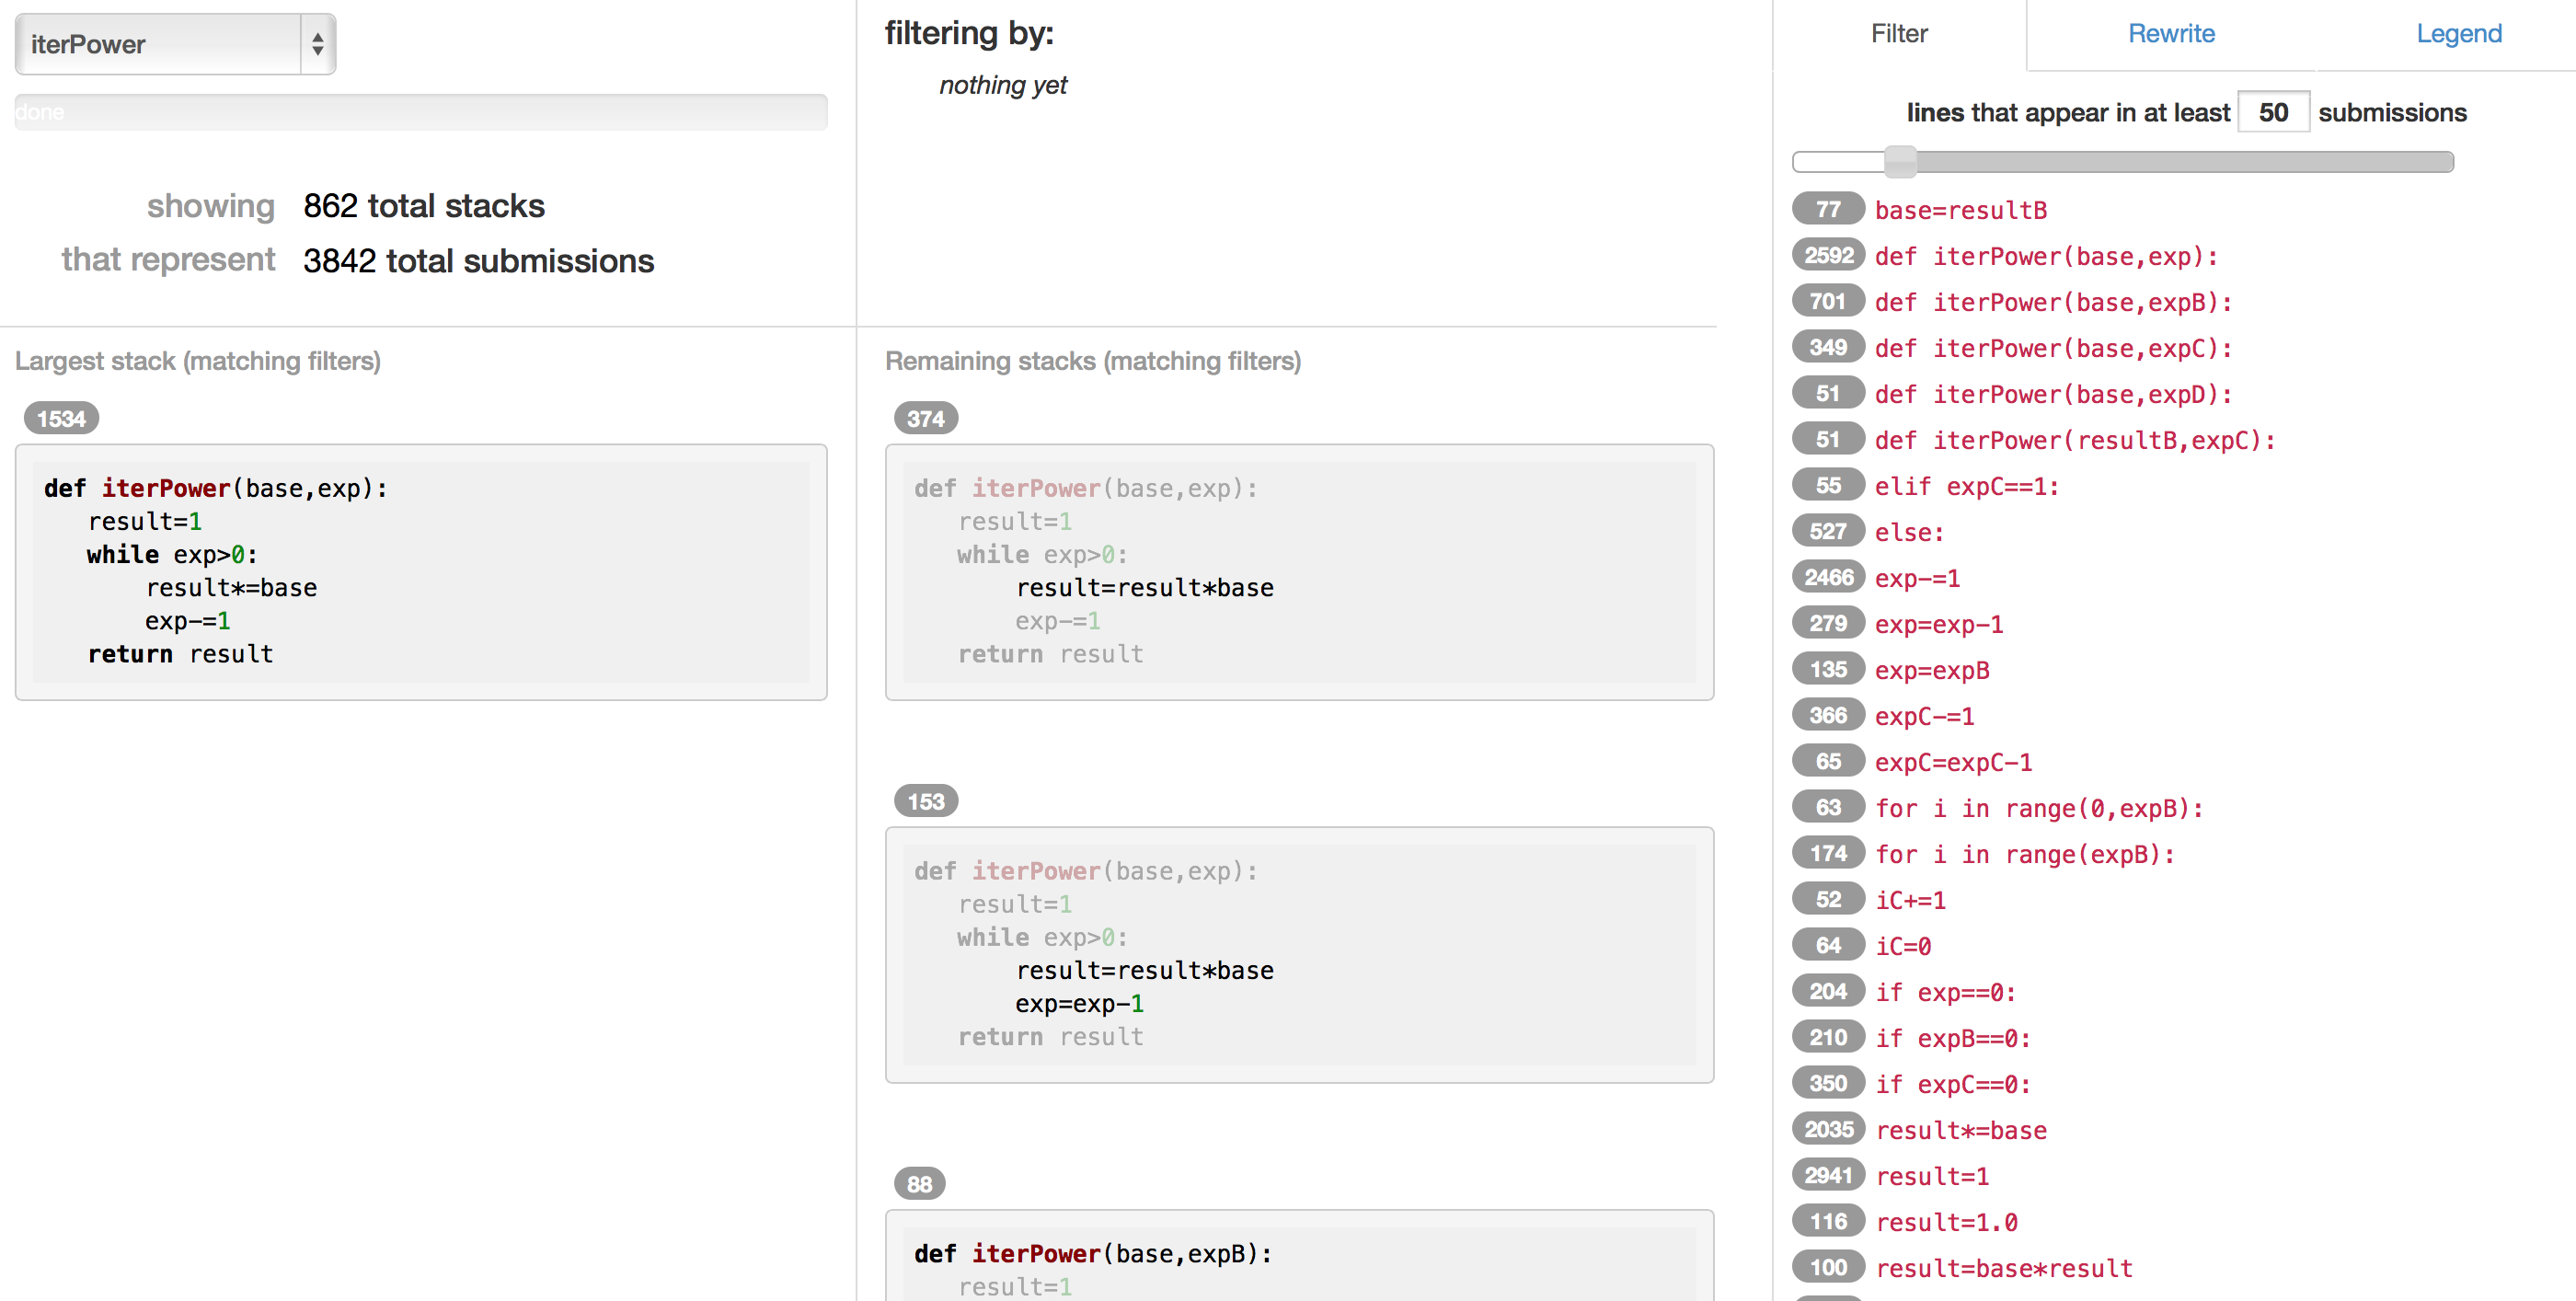
\includegraphics[width=1.0\linewidth]{Body/figures/overcode/interfaceScreenShot.png}
\caption{The OverCode user interface. The top left panel shows the number of clusters, called {\it stacks}, and the total number of solutions visualized. The next panel down in the first column shows the largest stack, while the second column shows the remaining stacks. The third column shows the lines of code in the platonic solutions and their frequencies.}
\label{overcode_fullinterface}
\end{figure*}

Sifting through thousands of solutions to understand their variation and find pedagogically valuable examples is a daunting task, even if the programming problems are simple and the solutions are only tens of lines of code long. Without tool support, a teacher may not read more than 50-100 of them before growing frustrated with the tedium of the task. Given this small sample size, teachers cannot be expected to develop a thorough understanding of the variety of strategies used to solve the problem, produce instructive feedback that is relevant to a large proportion of learners, or find unexpected interesting solutions.

An information visualization approach would enable teachers to explore the variation in solutions at scale. Existing techniques~\cite{gradingsigcse14,MOOCshop,codewebs} use a combination of clustering to group solutions that are semantically similar, and graph visualization to show the variation between these clusters. These clustering algorithms perform pairwise comparisons that are quadratic in both the number of solutions and in the size of each solution, which scales poorly to thousands of solutions. Graph visualization also struggles with how to label the graph node for a cluster, because it has been formed by a complex combination of code features. Without meaningful labels for clusters in the graph, the rich information in student solutions is lost and the ability of the teacher to understand variation is weakened.

This chapter presents OverCode, a system for visualizing and exploring the variation in thousands of programming solutions. OverCode is designed to visualize correct solutions, in the sense that they already passed the automatic grading tests typically used in a programming class at scale. The autograder cannot offer any further feedback on these correct solutions, and yet there may still be good and bad variations on correct solutions that are pedagogically valuable to highlight and discuss. OverCode aims to help teachers understand solution variation so that they can provide appropriate feedback to students at scale.

OverCode uses a novel human-interpretable solution clustering technique. The clustering process is linear in time with respect to both the number of solutions and the size of each solution. The platonic solution that represents each cluster is readable, executable, and describes every solution in that cluster in a deterministic way that accounts for both syntax and behavior on test cases. The platonic solutions are shown in a visualization that puts code front-and-center (Figure~\ref{overcode_fullinterface}). In the OverCode interface, teachers read through platonic solutions that each represent an entire cluster of solutions. The differences between clusters are highlighted to help teachers discover and understand the variations among solutions. Clusters can be filtered by the lines of code within them.  Clusters can also be merged together with {\em rewrite rules} that collapse variations that the teacher decides are unimportant. 

A cluster in OverCode is a set of solutions that perform the same computations, but may use different variable names or statement order.  OverCode uses a lightweight dynamic analysis to generate clusters, which scales linearly with the number of solutions. It clusters solutions whose variables take the same sequence of values when executed on test inputs and whose set of constituent lines of code are syntactically the same. 

An important component of this analysis is to rename variables that behave the same across different solutions. The renaming of variables serves three main purposes. First, it lets teachers create a mental mapping between variable names and their behavior which is consistent across the entire set of solutions. This may reduce the cognitive load for a teacher to understand different solutions. Second, it helps clustering by reducing variation between similar solutions. Finally, it also helps make the remaining differences between different solutions more salient. 

This chapter concludes by presenting two user studies with a total of 24 participants who each looked at thousands of solutions from an introductory programming MOOC, the OverCode interface is compared with a baseline interface that showed original unclustered solutions. When using OverCode, participants felt that they developed a better high-level view of the students' understandings and misconceptions. While participants did not necessarily read more lines of code in the OverCode interface than in the baseline, the code they did read came from clusters containing a greater percentage of all the submitted solutions. Participants also drafted mock class forum posts about common good and bad solutions. These forum posts were relevant to more student solutions when using OverCode as compared to the baseline. 

\section{OverCode} \label{overcode}
OverCode is an information visualization application for teachers to explore student solutions. OverCode uses the metaphor of solutions stacked on top of each other to denote a cluster of similar solutions. The top solution in the stack is the platonic solution that represents all the other solutions in the stack. The OverCode interface allows the teacher to scroll through, filter, and merge stacks of solutions. 

The platonic solutions that represent stacks are normalized in a novel way. Specifically, they have standardized formatting, no comments, and variable names that reflect the most popular naming choices across all solutions. They can be filtered by the normalized lines of code they contain and, through rewrite rules, modified and merged. They are the result of the normalization process applied to all student solutions in the OverCode analysis pipeline. %They can also be rewritten when teachers compose and apply \emph{rewrite rules}, which can eliminate differences between platonic solutions and therefore merge stacks that have become identical after the rewrite. 

%The OverCode interface was iteratively designed and developed based on continuous evaluation by the authors, feedback from teachers and peers, and by consulting principles from the information visualization literature. 
A screenshot of OverCode visualizing \codevar{iterPower}, one of the problems from our dataset, is shown in Figure~\ref{overcode_fullinterface}. In this section, the intended use cases and the user interface are described. In Section \ref{pipeline}, the backend program analysis pipeline is described in detail. 
\subsection{Target Users and Tasks}
The target users of OverCode are teaching staff of introductory programming courses. Teaching staff may be undergraduate lab assistants who help students debug their code; graduate students who grade assignments, help students debug, and manage recitations and course forums; and instructors who compose major course assessments. Teachers using OverCode may be looking for common misconceptions, creating a grading rubric, or choosing pedagogically valuable examples to review with students in a future lesson.

\subsubsection{Misconceptions and Holes in Student Knowledge}
Students just starting to learn programming can have a difficult time understanding the language constructs and different API methods. They may use them suboptimally, or in non-standard ways. OverCode may help instructors identify these common misconceptions and holes in knowledge, by highlighting the differences between stacks of solutions. Since the visualized solutions have already been tested and found correct by an autograder, these highlighted differences between platonic solutions may be convoluted variations in construct usage and API method choices that have not been flagged by the Python interpreter or caused the failure of a unit test. Convoluted code may suggest a misconception.

%\todo{DNHT: Rob: it would be great to show example code for these tasks, ideally showing them in OverCode -- can you mine any examples from your thesis defense talk?}

\subsubsection{Grading Rubrics}
It is a difficult task to create grading rubrics for checking properties such as design and style of solutions. Therefore most autograders resort to checking only functional correctness of solutions by testing them against a test suite of input-output pairs. OverCode enables teachers to identify the style, structure, and relative frequency of the variation within correct solutions. Unlike traditional ways of creating a grading rubric, where an instructor may go through a set of solutions, revising the rubric along the way, instructors can use OverCode to first get a high-level overview of the variations before designing a corresponding rubric. Teachers may also see incorrect solutions not caught by the autograder.

\subsubsection{Pedagogically Valuable Examples} 
There can be a variety of ways to solve a given problem and express it in code. If an assignment allows students to generate different solutions, e.g., recursive or iterative, to fulfill the same input-output behavior, OverCode will show separate stacks for each of these different solutions, as well as stacks for every variant of those solutions. OverCode helps teachers filter through solutions to find different examples of solutions to the same problem, which may be pedagogically valuable. According to variation theory ~\cite{marton13}, students can learn through concrete examples of these multiple solutions, which vary along different conceptual dimensions.
\subsection{User Interface}

The OverCode user interface is the product of an iterative design process with multiple stages, including paper prototypes and low-fidelity prototypes rendered in a web browser. User interface design experts and programming teachers critiqued initial prototypes. While exploring the low-fidelity prototypes, the teachers talked aloud about their hopes for what the tool could do, frustrations with its current form, and their frustrations with existing solution-viewing tools and processes. This feedback was incorporated into the final design.

The OverCode user interface is divided into three columns. The top-left panel in the first column shows the problem name, the \emph{done} progress bar, the number of stacks, the number of visualized stacks given the current filters and rewrite rules, and the total number of solutions those visualized stacks contain. The panel below shows the largest stack of solutions. Side by side with the largest stack, the remaining stacks appear in the second panel. Through scrolling, any stack can be horizontally aligned with the largest stack for easier comparison. The third panel has three different tabs that provide static and dynamic information about the solutions, and the ability to filter and combine stacks. 

As shown in Figure~\ref{overcode_fullinterface}, the default tab shows a list of lines of code that occur in different platonic solutions together with their corresponding frequencies. The stacks can be filtered based on the occurrence of one or more lines (Filter tab). The column also has tabs for \emph{Rewrite} and \emph{Legend}. The Rewrite tab allows a teacher to provide rewrite rules to collapse different stacks with small differences into a larger single stack. The Legend tab shows the dynamic values that different program variables take during the execution of programs over a test case. %We now describe different features of OverCode in more detail.
%\todo{ROB:maybe the TOCHI paper didn't have space for screenshots of these, but your thesis needs them}

% \begin{figure}
% 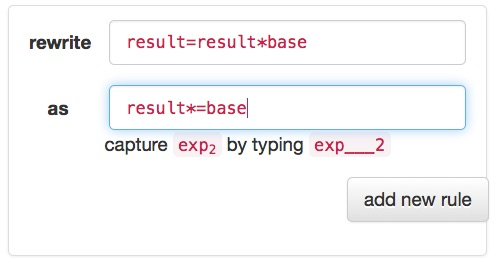
\includegraphics[width=0.5\paperwidth]{Body/figures/overcode/rewrite_rule.jpg}
% \caption{UI for adding rewrite rules.}
% \label{fig:rewriterule}
% \end{figure}

\subsubsection{Stacks} A stack in OverCode denotes a set of similar solutions that are grouped together based on a similarity criterion defined in Section \ref{pipeline}. For example, a stack for the \codevar{iterPower} problem is shown in Figure~\ref{stacks}(a). The size of each stack, i.e., the number of solutions in a stack, is shown in a pillbox at the top-left corner of the stack. Stacks are listed in the scrollable second panel from largest to smallest. The solution on the top of the stack is a platonic solution that describes all the solutions in the stack. See Section \ref{pipeline} for details on the normalizing process that produces platonic solutions.

Each stack can also be clicked. After clicking a stack, the border color of the stack changes and the \emph{done} progress bar is updated to reflect the percentage of total solutions clicked, as shown in Figure~\ref{stacks}(b). This feature is intended to help teachers remember which stacks they have already read or analyzed, and keep track of their progress. Clicking on a large stack, which represents a significant fraction of the total solutions, is reflected by a large change in the \emph{done} progress bar. Double clicking on any stack reveals the raw solutions that belong to that stack. This last feature was added after user testing.% \todo{add that now the raw solutions inside the stack are also displayed, but this was not included during user study tests}

\begin{figure*}[htpb]
\begin{tabular}{c | c}
\begin{minipage}{.5\linewidth}
\centering
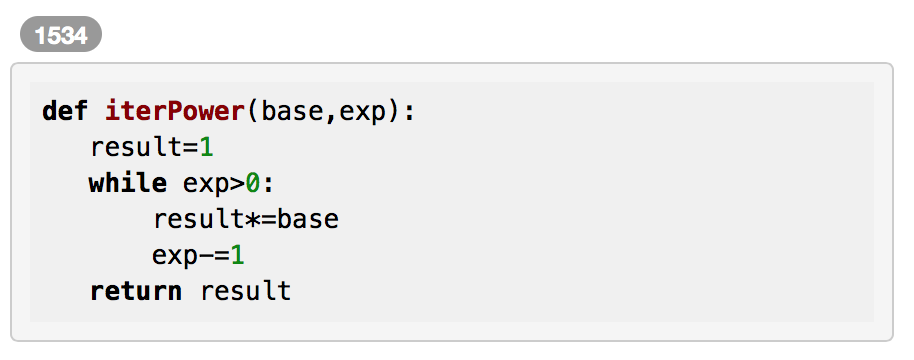
\includegraphics[width=0.95\linewidth]{Body/figures/overcode/stackScreenShot.png}
\end{minipage}
&
\begin{minipage}{.5\linewidth}
\centering
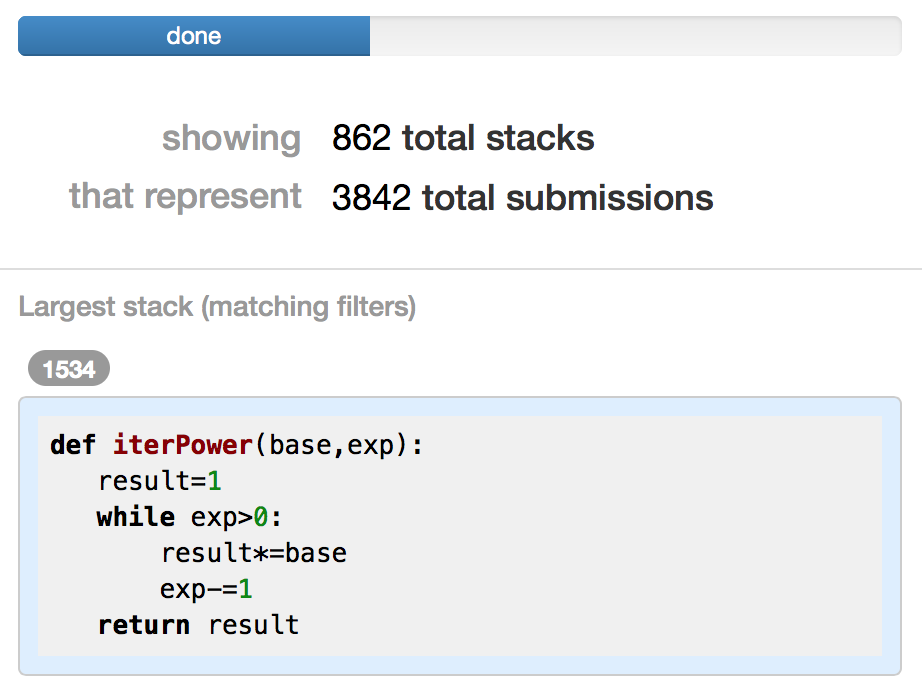
\includegraphics[width=0.95\linewidth]{Body/figures/overcode/checkDone.png}
\end{minipage}
\\
(a) & (b)
\end{tabular}
\caption{(a) A stack of 1534 similar \codevar{iterPower} solutions. (b) After clicking a stack, the border color of the stack changes and the done progress bar denotes the corresponding fraction of solutions that have been checked.}
\label{stacks}
\end{figure*}

\subsubsection{Showing Differences between Stacks} OverCode allows teachers to compare smaller stacks, shown in the second column, with the largest stack, shown in the first column. The lines of code in the second column that also appear in the set of lines in the largest stack are dimmed so that only the differences between the smaller stacks and the largest stack are apparent. For example, Figure~\ref{stackdifferences} shows the differences between the platonic solutions of the two largest stacks. In earlier iterations of the user interface, lines in stacks not shared with the largest stack were highlighted in yellow, but this produced a lot of visual noise. By dimming the lines in stacks that \textit{are} shared with the largest stack, the visible noise is reduced, while still keeping differences between stacks salient.

\begin{figure*}
\centering
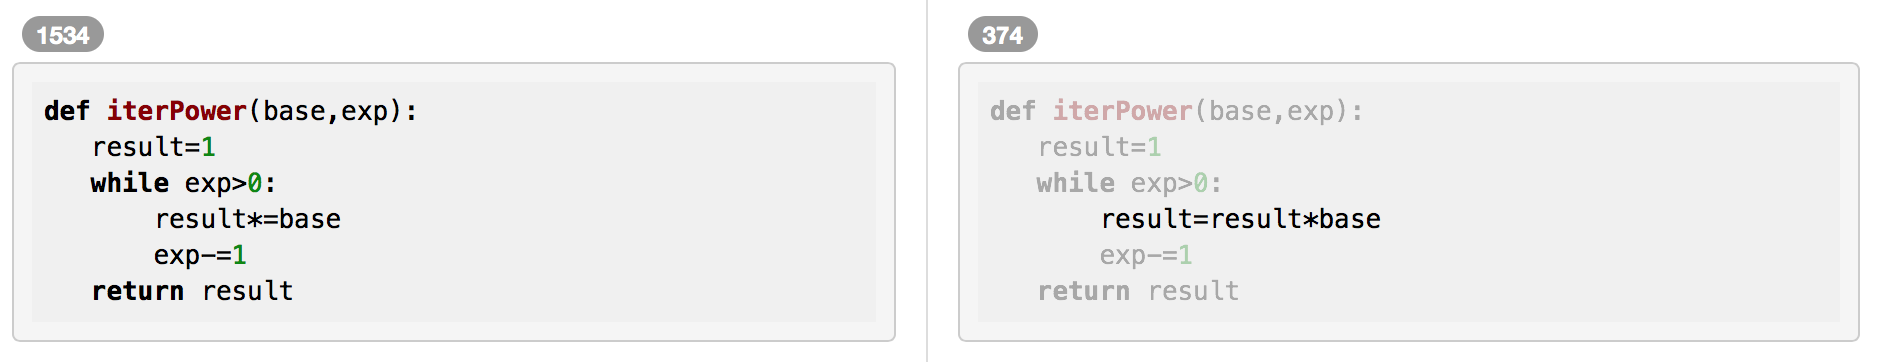
\includegraphics[scale=0.42]{Body/figures/overcode/lineFadingScreenshot}
\caption{Similar lines of code between two stacks are dimmed out such that only differences between the two stacks are apparent.}
\label{stackdifferences}
\end{figure*}



\subsubsection{Filtering Stacks by Lines of Code} The third column of OverCode shows the list of lines of code occurring in the solutions together with their frequencies (numbered pillboxes). The interface has a slider that can be used to change the threshold value, which denotes the number of solutions in which a line should appear for it to be included in the list. For example, by dragging the slider to $200$ in Figure~\ref{linefilter}(a), OverCode only shows lines of code that are present in at least $200$ solutions. This feature was added as a response to the length of the unfiltered list of code lines, which was long enough to make skimming for common code lines difficult.

Users can filter the stacks by selecting one or more lines of code from the list. After each selection, only stacks whose platonic solutions have those selected lines of code are shown. Figure~\ref{linefilter}(b) shows a filtering of stacks that have a \codevar{for} loop, specifically the line of code \codevar{for i in range(expB)}, and that assign $1$ to the variable \codevar{result}.

\begin{figure*}[htpb]
\begin{tabular}{c | c}
\begin{minipage}{.48\linewidth}
\centering
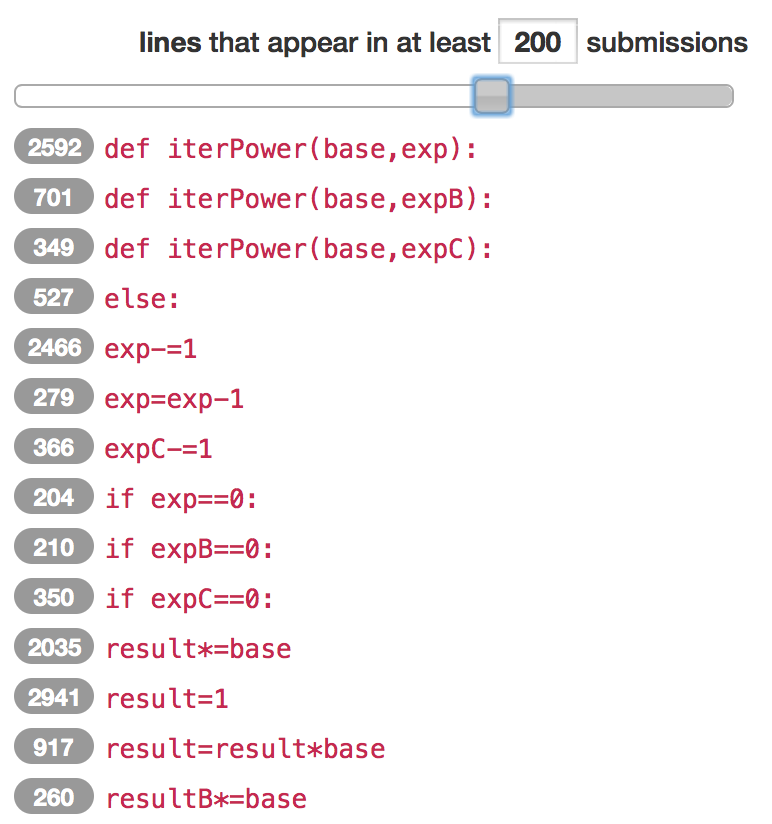
\includegraphics[scale=0.5]{Body/figures/overcode/lineSlider.png}
\end{minipage}
&
\begin{minipage}{.52\linewidth}
\centering
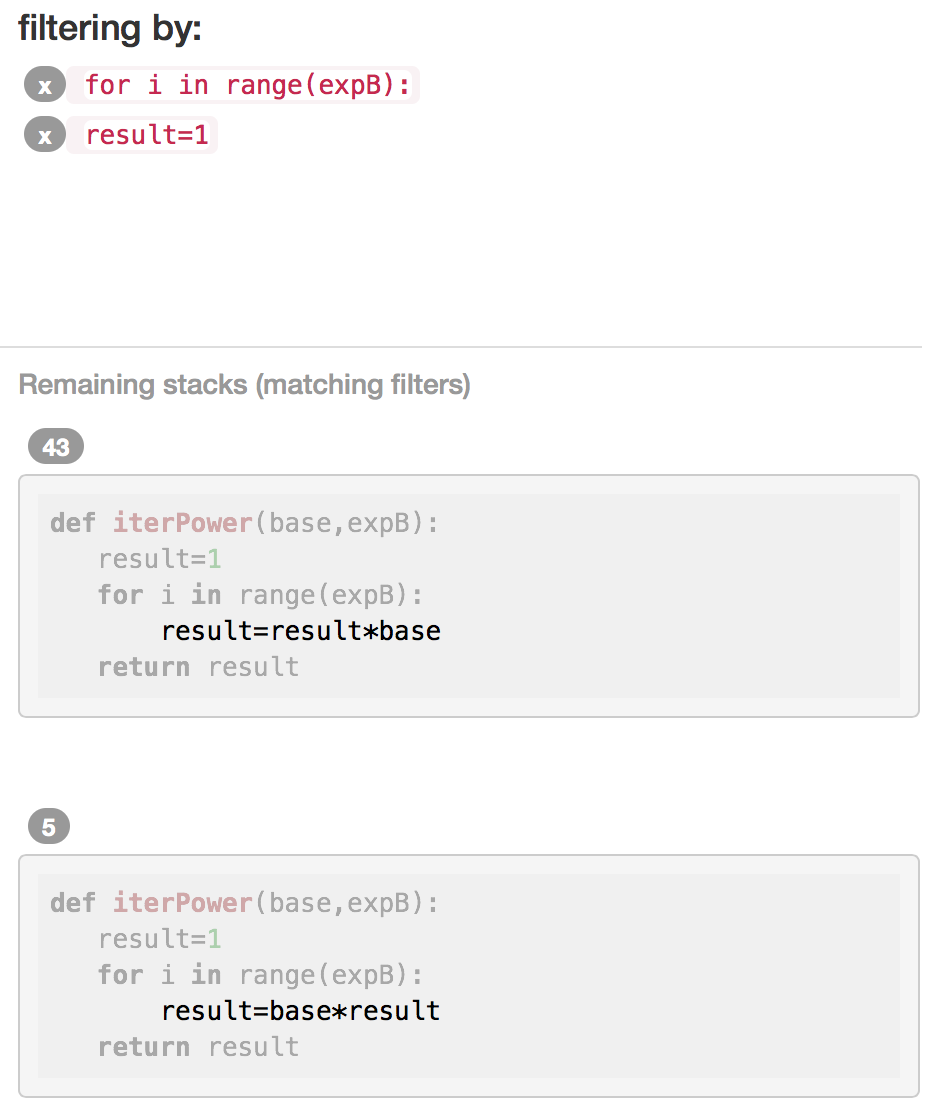
\includegraphics[scale=0.40]{Body/figures/overcode/lineFilter.png}
\end{minipage}
\\
(a) & (b)
\end{tabular}
\caption{(a) The slider allows filtering of the list of lines of code by the number of solutions in which they appear. (b) Clicking on a line of code adds it to the list of lines by which the stacks are filtered.}
\label{linefilter}
\end{figure*}

\subsubsection{Rewrite Rules} There are often small differences between the platonic solutions that can lead to a large number of stacks for a teacher to review. OverCode provides \emph{rewrite rules} by which teachers can collapse these differences and ignore variation they do not need to see. This feature comes from experience with early prototypes. After observing a difference between stacks, like the use of \codevar{xrange} instead of \codevar{range}, teachers wanted to ignore that difference in order to more easily find other differences.

A rewrite rule is described with a left hand side and a right hand side as shown in Figure~\ref{rewriterule}(a). The semantics of a rewrite rule is to replace all occurrences of the left-hand side expression in the platonic solutions with the corresponding right-hand side. As the rewrite rules are entered, OverCode presents a preview of the changes in the platonic solutions as shown in Figure~\ref{rewriterule}(b). After the application of the rewrite rules, OverCode collapses stacks that now have the same platonic solutions because of the rewrites. For example, after the application of the rewrite rule in Figure~\ref{rewriterule}(a), OverCode collapses the two biggest iterPower stacks from Figure~\ref{overcode_fullinterface} of sizes $1534$ and $374$, respectively, into a single stack of size $1908$. Other pairs of stacks whose differences have now been removed by the rewrite rule are also collapsed into single stacks. As shown in Figure~\ref{afterrewrite}(a), the number of stacks now drop from $862$ to $814$.

\begin{figure*}[htpb]
\begin{tabular}{c | c}
\begin{minipage}{.5\linewidth}
\centering
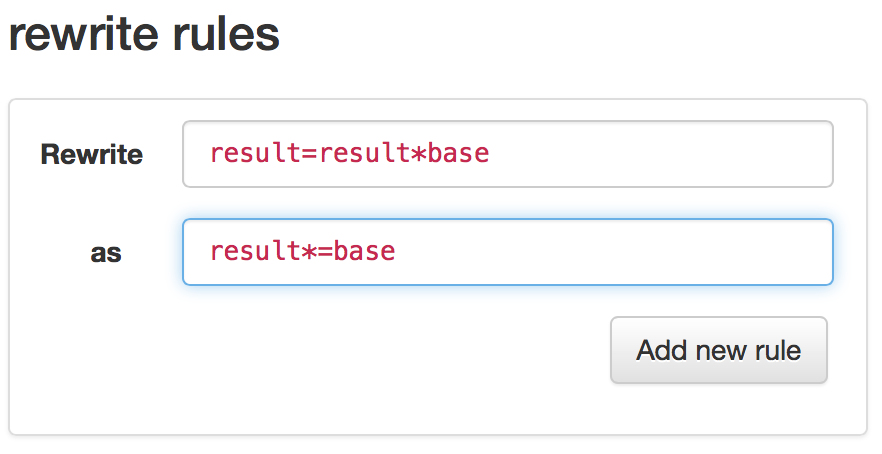
\includegraphics[scale=0.45]{Body/figures/overcode/rewriteRuleScreenshot.png}
\end{minipage}
&
\begin{minipage}{.5\linewidth}
\centering
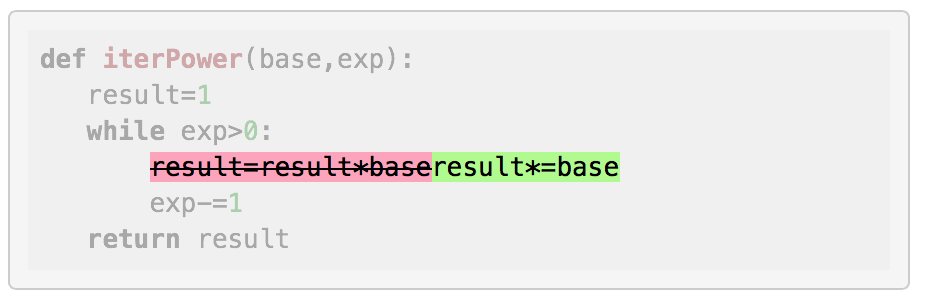
\includegraphics[scale=0.40]{Body/figures/overcode/rewritePreviewScreenShot.png}
\end{minipage}
\\
(a) & (b)
\end{tabular}
\caption{(a) An example rewrite rule to replace all occurrences of statement \codevar{result = base * result} with \codevar{result *= base}. (b) The preview of the changes in the platonic solutions because of the application of the rewrite rule.}
\label{rewriterule}
\end{figure*}

\begin{figure*}[htpb]
\begin{tabular}{c | c}
\begin{minipage}{.5\linewidth}
\centering
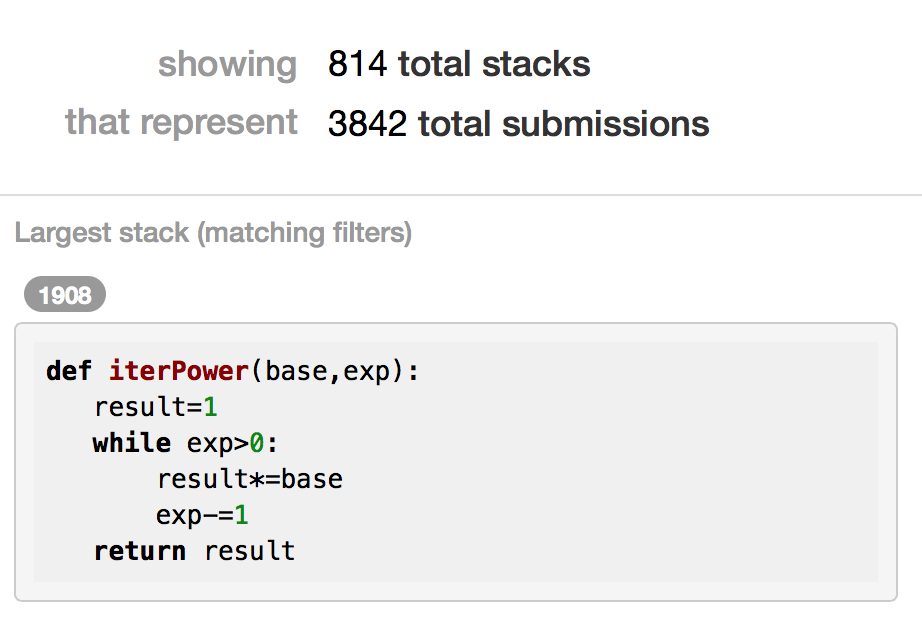
\includegraphics[scale=0.4]{Body/figures/overcode/afterrewrite.png}
\end{minipage}
&
\begin{minipage}{.5\linewidth}
\centering
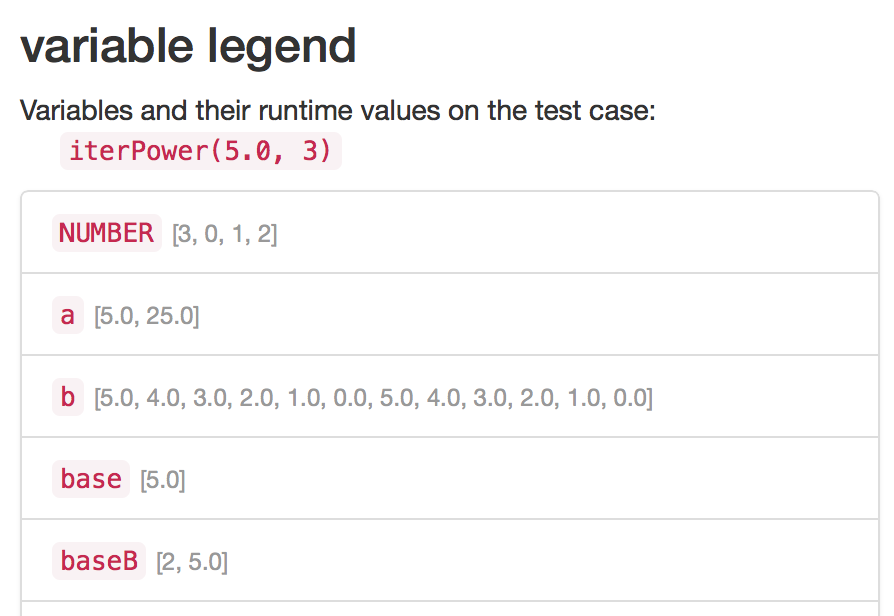
\includegraphics[scale=0.4]{Body/figures/overcode/variableLegend.png}
\end{minipage}
\\
(a) & (b)
\end{tabular}
\caption{(a) The merging of stacks after application of the rewrite rule shown in Figure~\ref{rewriterule}. (b) The variable legend shows the sequence of dynamic values that all program variables in normalized solutions take over the course of execution on a given test case.}
\label{afterrewrite}
\end{figure*}

\subsubsection{Variable Legends} OverCode also shows the sequence of values that variables in the platonic solutions take on, over the course of their execution on a test case. As described in Section~\ref{pipeline}, a variable is identified by the sequence of values it takes on during the execution of the test case. Figure~\ref{afterrewrite}(b) shows a snapshot of the variable values for the \codevar{iterPower} problem. The goal of presenting this dynamic information associated with common variable names is intended to help teachers (1) understand the behavior of each platonic solution without having to mentally execute it on a test case and (2) further explore the variations among solutions that do not have the same common variables. When this legend was originally added to the user interface, clicking on a common variable name would filter for all solutions that contained an instance of that variable. Some pilot users found this feature confusing, rather than empowering. As a result, it was removed from OverCode before running both user studies. At least one study participant, upon realizing the value of the legend, wished that the original click-to-filter-by-variable functionality existed; it may be reinstated in future versions.

\section{Implementation} \label{pipeline}
The OverCode user interface depends on an analysis pipeline that normalizes solutions in a manner designed for human readability. The pipeline then creates stacks of solutions that have become identical through the normalizing process. The pipeline accepts, as input, a set of solutions, expressed as function definitions for $f(a,...)$, and a set of test cases. Solutions that enter the pipeline are referred to as \emph{raw}, and the solutions that exit the pipeline as \emph{normal}. Examples, beginning with \codevar{iterPower}, are presented below to illustrate this pipeline.

\subsection{Analysis Pipeline}
OverCode is currently implemented for Python, but the pipeline steps described below could be readily generalized to other languages commonly used to teach programming.

{\bf 1. Reformat solutions.} For a consistent appearance, the solutions are reformatted with the PythonTidy package\footnote{Created by Charles Curtis Rhode. \url{https://pypi.python.org/pypi/PythonTidy/}} to have consistent line indentation and token spacing. Comments and empty lines are also removed. These steps not only make solutions more readable, but also allow exact string matches between solutions, after additional normalizing steps later in the pipeline. Although comments can contain valuable information, the variation in comments is so great that clustering and summarizing them will require significant additional design, which remains future work. Figure~\ref{fig:reformat} illustrates the effect of this reformatting.
\begin{figure}
\begin{tabular}{ll}
{\bf Raw Solution A} & {\bf Reformatted Solution A} \\
\begin{minipage}{0.5\linewidth}
\begin{lstlisting}[basicstyle=\linespread{1.0}\ttfamily\footnotesize,language=python]
def iterPower(base, exp):
    '''
    base: int or float.
    exp: int >= 0
    returns: int or float, base^exp
    '''
    result = 1
    for i in range(exp):
        result *= base
    return result
\end{lstlisting}
\end{minipage}
&
\begin{minipage}{0.5\linewidth}
\begin{lstlisting}[basicstyle=\linespread{1.0}\ttfamily\footnotesize,language=python]
def iterPower(base,exp):
    result=1
    for i in range(exp):
        result*=base
    return result
\end{lstlisting}
\end{minipage}
\end{tabular}
\caption{A student solution before and after reformatting.}
\label{fig:reformat}
\end{figure}

{\bf 2. Execute solutions.} Each solution is on the same test case(s). During each step of the execution for each test case, the names and values of local and global variables, and also return values from functions, are recorded as a program trace adapted from the execution logger written by Philip Guo~\cite{pgbovineOPT}. There is one program trace per solution per test case. Included for the purpose of illustrating this pipeline, the examples in the figures that follow are derived from executing definitions of \codevar{iterPower} on a \codevar{base} of $5.0$ and an \codevar{exp} of $3$, as illustrated in Figure~\ref{fig:testcase}.
\begin{figure}
\begin{tabular}{l}
{\bf Student Solution with Test Case} \\
\begin{minipage}{0.5\linewidth}
\begin{lstlisting}[basicstyle=\linespread{1.0}\ttfamily\footnotesize,language=python]
def iterPower(base,exp):
    #student solution here
iterPower(5.0, 3)
\end{lstlisting}
\end{minipage} 
\end{tabular}
\caption{Illustration of running a (dummy) \texttt{iterPower} solution on a test case.}
\label{fig:testcase}
\end{figure}

%This sequence of values excludes consecutive duplicates. 
{\bf 3. Extract variable sequences.} For each variable in a program trace, the pipeline extracts the sequence of distinct values it takes on. Figure~\ref{fig:extractsequence} shows the program trace for a solution run on a test case, as well as the extracted sequences of distinct values for each variable. Variable sequence extraction also works for purely functional programs, in which variables are never reassigned, because each recursive invocation is treated as if new values are given to its parameter variables. For example, in spite of the fact that the \codevar{iterPower} problem asked students to compute the exponential $\codevar{base}^\codevar{exp}$ iteratively, $60$ of the $3842$ \codevar{iterPower} solutions in the dataset were in fact recursive. One of these recursive examples is shown in Figure~\ref{fig:recursiveTrace}, along with the variable sequences extracted.
\begin{figure}
\begin{tabular}{ll}
{\bf Solution A with Test Case} & {\bf Program Trace for Solution A} \\
\begin{minipage}{0.35\linewidth}
\begin{lstlisting}[basicstyle=\linespread{1.0}\ttfamily\footnotesize,language=python]
def iterPower(base,exp):
    result=1
    for i in range(exp):
        result*=base
    return result
iterPower(5.0, 3)
\end{lstlisting}
\end{minipage} &
\begin{minipage}{0.6\linewidth}
\begin{lstlisting}[basicstyle=\linespread{1.0}\ttfamily\footnotesize,language=python,linebackgroundcolor={\lstcolorlines[gray!20]{2,4,6,8,10,12,14,16,18}}]
iterPower(5.0, 3)
 base : 5.0, exp : 3
result=1
 base : 5.0, exp : 3, result : 1 
for i in range(exp):
 base : 5.0, exp : 3, result : 1, i : 0
result*=base
 base : 5.0, exp : 3, result : 5.0, i : 0 
for i in range(exp):
 base : 5.0, exp : 3, result : 5.0, i : 1
result*=base 
 base : 5.0, exp : 3, result : 25.0, i : 1 
for i in range(exp):
 base : 5.0, exp : 3, result : 25.0, i : 2 
result*=base
 base : 5.0, exp : 3, result : 125.0, i : 2
return result
 value returned: 125.0
\end{lstlisting}
\end{minipage} 
\\
& {\bf Variable Sequences for Solution A} \\
&
\begin{minipage}{0.6\linewidth}
\begin{lstlisting}[language=python]
base: 5.0
exp: 3
result: 1, 5.0, 25.0, 125.0
i: 0, 1, 2
\end{lstlisting}
\end{minipage}
\end{tabular}
\caption{A student solution, its program trace when running on the test case \texttt{iterPower(5.0,3)}, and the sequence of values extracted from the trace for each variable.}
\label{fig:extractsequence}
\end{figure}

\begin{figure}
\begin{tabular}{ll}
{\bf Recursive Example} & {\bf Program Trace} \\
 % & {\bf for Recursive Example} \\
\begin{minipage}{0.5\linewidth}
\begin{lstlisting}[basicstyle=\linespread{1.0}\ttfamily\footnotesize,language=python]
def iterPower(base,exp):
   if exp==0:
       return 1
   else:
       return base*iterPower(base,exp-1)
iterPower(5.0, 3)
\end{lstlisting}
\end{minipage} &
\begin{minipage}{0.4\linewidth}
\begin{lstlisting}[basicstyle=\linespread{1.0}\ttfamily\footnotesize,language=python,linebackgroundcolor={\lstcolorlines[gray!20]{2,4,6,8,10,12,14,16,18,20,22,24,26,28,30}}]
iterPower(5.0, 3)
 base : 5.0, exp : 3
if exp==0:
 base : 5.0, exp : 3 
return base*iterPower(base,exp-1)
 base : 5.0, exp : 3 
iterPower(5.0, 2)
 base : 5.0, exp : 2
if exp==0: 
 base : 5.0, exp : 2 
return base*iterPower(base,exp-1)
 base : 5.0, exp : 2
iterPower(5.0, 1)
 base : 5.0, exp : 1
if exp==0:
 base : 5.0, exp : 1
return base*iterPower(base,exp-1)
 base : 5.0, exp : 1
iterPower(5.0, 0)
 base : 5.0, exp : 0
if exp==0:
 base : 5.0, exp : 0
return 1
 base : 5.0, exp : 0
return base*1
 base : 5.0, exp : 1
return base*5
 base : 5.0, exp : 2
return base*25
 base : 5.0, exp : 3
value returned: 125.0
\end{lstlisting}
\end{minipage} 
\\
& {\bf Variable Sequences} \\
% & {\bf for Recursive Example} \\
&
\begin{minipage}{0.5\linewidth}
\begin{lstlisting}[language=python]
base: 5.0
exp: 3, 2, 1, 0, 1, 2, 3
\end{lstlisting}
\end{minipage}
\end{tabular}
\caption{A recursive solution to the same programming problem, its program trace when executing on \texttt{iterPower(5.0,3)}, and the extracted sequences of values for each variable.}
\label{fig:recursiveTrace}
\end{figure}


{\bf 4. Identify common variables.} The pipeline analyzes all program traces, identifying which variable value sequences are identical. Variables that have identical sequences of values across two or more program traces are referred to as {\it common variables}. Variables which occur in only one program trace are called {\it unique variables}. This is illustrated in Figures~\ref{fig:commik} and~\ref{fig:allvars}.
\begin{figure}
\begin{tabular}{ll}
{\bf Solution B with Test Case} & {\bf Variable Sequences for Solution B} \\
\begin{minipage}{0.5\linewidth}
\begin{lstlisting}[basicstyle=\linespread{1.0}\ttfamily\footnotesize,language=python]
def iterPower(base,exp):
    r=1
    for k in xrange(exp):
        r=r*base
    return r
iterPower(5.0, 3)
\end{lstlisting}
\end{minipage}
&
\begin{minipage}{0.5\linewidth}
\begin{lstlisting}[language=python]
base: 5.0
exp: 3
r: 1, 5.0, 25.0, 125.0
k: 0, 1, 2
\end{lstlisting}
\end{minipage} \\
{\bf Solution C with Test Case} & {\bf Variable Sequences for Solution C} \\
\begin{minipage}{0.5\linewidth}
\begin{lstlisting}[basicstyle=\linespread{1.0}\ttfamily\footnotesize,language=python]
def iterPower(base,exp):
   result=1
   while exp>0:
       result*=base
       exp-=1
   return result
iterPower(5.0, 3)
\end{lstlisting}
\end{minipage}
&
\begin{minipage}{0.5\linewidth}
\begin{lstlisting}[language=python]
base : 5.0
exp: 3
result : 1, 5.0, 25.0, 125.0
exp : 3, 2, 1, 0
\end{lstlisting}
\end{minipage}
\end{tabular}
\caption{\codevar{i} and \codevar{k} take on the same sequence of values, $0$ then $1$ then $2$, in Solution A and B. They are therefore considered the same {\it common variable}.}
\label{fig:commik}
\end{figure}
\begin{figure}
{\bf Common variables} in solutions A, B, and C:
\begin{itemize}
\item \texttt{5.0}:
\begin{itemize}
\item \texttt{base} (Solutions A, B, C)
\end{itemize}
\item \texttt{3}:
\begin{itemize}
\item \texttt{exp} (Solutions A, B) 
\end{itemize}
\item \texttt{1, 5.0, 25.0, 125.0}: 
\begin{itemize}
\item \texttt{result} (Solutions A, C)
\item \texttt{r} (Student B)
\end{itemize}
\item \texttt{0,1,2}:
\begin{itemize}
\item \texttt{i} (Solution A) 
\item \texttt{k} (Student B)
\end{itemize}
\end{itemize}
{\bf Unique variables} in solutions A, B, and C:
\begin{itemize}
\item \texttt{3,2,1,0}:
\begin{itemize}
\item \texttt{exp} (Student C)
\end{itemize}
\end{itemize}
\caption{Common and uncommon variables found across the solutions in the previous figure.}
\label{fig:allvars}
\end{figure}

{\bf 5. Rename common and unique variables.} A common variable may have a different name in each program trace. In this step, the common variable is renamed to the name that is given most often to that common variable across all program traces. 

There are exceptions made to avoid name collisions. For example, the unique variable in the previous pipeline step was originally named \codevar{exp}. As shown in Figure~\ref{fig:uniqcomm}, OverCode appends a double underscore as a modifier to resolve a name collision with the common variable of the same name. This is referred to as a unique/common collision.
\begin{figure}
\begin{tabular}{ll}
{\bf Common Variables, Named} & {\bf Unique Variables, Named} \\
\begin{minipage}{0.5\linewidth}
\begin{itemize}
\item \texttt{base: 5.0} 
\item \texttt{exp: 3} 
\item \texttt{result: 1, 5.0, 25.0, 125.0}
\item \texttt{i: 0,1,2} (common name tie broken by random choice)
\end{itemize}
\end{minipage}
&
\begin{minipage}{0.5\linewidth}
\begin{itemize}
\item \begin{verbatim} exp__: 3,2,1,0 \end{verbatim}
\end{itemize}
\end{minipage}

\end{tabular}
\caption{The unique variable in the previous pipeline step was originally named \codevar{exp}. OverCode appends a double underscore as a modifier to resolve a name collision with the common variable of the same name. This is referred to as a unique/common collision.}
\label{fig:uniqcomm}
\end{figure}

After common and unique variables in the solutions are renamed, the solutions are now called {\it normal}, as shown in Figure~\ref{fig:normalcode}.
\begin{figure}
\begin{tabular}{ll}

{\bf Normal Solution A} & {\bf Normal Solution B} \\ 

\begin{minipage}{0.5\linewidth}
\begin{lstlisting}[basicstyle=\linespread{1.0}\ttfamily\footnotesize,language=python]
def iterPower(base,exp):
    result=1
    for i in range(exp):
        result*=base
    return result
\end{lstlisting}
\end{minipage} &
\begin{minipage}{0.5\linewidth}
\begin{lstlisting}[basicstyle=\linespread{1.0}\ttfamily\footnotesize,language=python]
def iterPower(base,exp):
    result=1
    for i in xrange(exp):
        result=result*base
    return result
\end{lstlisting}
\end{minipage}
\\
{\bf Normal Solution C} &  \\
\begin{minipage}{0.5\linewidth}
\begin{lstlisting}[basicstyle=\linespread{1.0}\ttfamily\footnotesize,language=python]
def iterPower(base,exp__):
   result=1
   while exp__>0:
       result*=base
       exp__-=1
   return result
\end{lstlisting}
\end{minipage}
& \\
\end{tabular}
\caption{Normalized solutions after variable renaming.}
\label{fig:normalcode}
\end{figure}

{\bf 6. Make stacks.} The pipeline iterates through the normal solutions, making stacks of solutions that share an identical {\it set} of lines of code. The pipeline compares sets of lines of code because then solutions with arbitrarily ordered lines that do not depend on each other can still fall into the same stack. (Recall that the variables in these lines of code have already been renamed based on their dynamic behavior, and all the solutions have already been marked input-output correct by an autograder, prior to this pipeline.) The platonic solution that represents the stack is randomly chosen from within the stack, because all the normal solutions within the stack are identical, with the possible exception of the order of their statements. 

In the examples in Figure~\ref{fig:makingstacks}, the normal C and D solutions have the same set of lines, and both provide correct output, with respect to the autograder. Therefore, the difference in order of the statements between the two solutions is not communicated to the teacher. The two solutions are put in the same stack, with one solution arbitrarily chosen as the visible normalized code. However, since Solution A and B use different functions, i.e., \codevar{xrange} vs. \codevar{range}, and different operators, i.e., \codevar{*=} vs. \codevar{=,*}, the pipeline puts them in separate stacks.
%\vspace{10mm}
\begin{figure}
\begin{tabular}{l|l}
{\bf Stack 1} Normal Solution A & {\bf Stack 2} Normal Solution B \\
\begin{minipage}{0.5\linewidth}
\begin{lstlisting}[basicstyle=\linespread{1.0}\ttfamily\footnotesize,language=python,linebackgroundcolor={\lstcolorlines[gray!20]{3,4}}]
def iterPower(base,exp):
    result=1
    for i in range(exp):
        result*=base
    return result
\end{lstlisting}
\end{minipage}
&
\begin{minipage}{0.5\linewidth}
\begin{lstlisting}[basicstyle=\linespread{1.0}\ttfamily\footnotesize,language=python,linebackgroundcolor={\lstcolorlines[gray!20]{3,4}}]
def iterPower(base,exp):
    result=1
    for i in xrange(exp):
        result=result*base
    return result
\end{lstlisting}
\end{minipage}
\end{tabular}
\begin{tabular}{ll}
\hline
\\
{\bf Stack 3} Normal Solution C & {\bf Stack 3} Normal Solution D  \\
\begin{minipage}{0.5\linewidth}
\begin{lstlisting}[basicstyle=\linespread{1.0}\ttfamily\footnotesize,language=python,linebackgroundcolor={\lstcolorlines[mygray]{4,5}}]
def iterPower(base,exp__):
    result=1
    while exp__>0:
        result=result*base
        exp__-=1
    return result
\end{lstlisting}
\end{minipage}
&
\begin{minipage}{0.5\linewidth}
\begin{lstlisting}[basicstyle=\linespread{1.0}\ttfamily\footnotesize,language=python,linebackgroundcolor={\lstcolorlines[mygray]{4,5}}]
def iterPower(base,exp__):
    result=1
    while exp__>0:
        exp__-=1
        result=result*base
    return result
\end{lstlisting}
\end{minipage}
\end{tabular}
\caption{Four solutions collapsed into three stacks.}
\label{fig:makingstacks}
\end{figure}
Some programming problems have no deadline, and new solutions are submitted intermittently. The entire pipeline does not need to be rerun to normalize a new solution and restack all the solutions in the dataset. The pipeline has been split into two phases: solution preprocessing and batch processing. During preprocessing, each solution formatting is standardized and all comments are removed. It is then executed on one or more test cases, which makes the resulting normalization more robust to any individual poorly chosen test case. The full program trace and output is recorded for every test case. 

This logging of solution execution can be one of the longer steps in the OverCode analysis pipeline, so preprocessing occurs once per solution and is saved in its own pickle file. New solutions can be preprocessed once, without affecting previously preprocessed solutions. Batch processing takes, as input, all the existing preprocessed results and normalizes variable names. This must occur as a batch operation because variable renaming depends on the behavior and name of every variable in every solution.

The program tracing \cite{pgbovineOPT} and renaming scripts occasionally generate errors while processing a solution. For example, the script may not have code to handle a particular but rare Python construct. Errors thrown by the scripts drive their development and are helpful for debugging. When errors occur while processing a particular solution, they are excluded from our analysis. Less than five percent of the solutions in each of the three problem datasets are excluded.

\subsection{Variable Renaming Details and Limitations} \label{repercussions}

There are three distinct types of name collisions possible when renaming variables to be consistent across multiple solutions. The first, referred to here as a {\it common/common} collision, occurs when two common variables (with different variable sequences) have the same common name. The second, referred to here as a {\it multiple instances} collision, occurs when there are multiple different instances of the same common variable in a solution. The third and final collision, referred to as a {\it unique/common} collision, occurs when the name of a unique variable collides with the name of a common variable.

{\bf Common/common collision.} If common variables $cv_{1}$ and $cv_{2}$ are both most frequently named $i$ across all program traces, the pipeline appends a modifier to the name of the less frequently used common variable. For example, if 500 program traces have an instance of $cv_{1}$ and only 250 program traces have an instance of $cv_{2}$, $cv_{1}$ will be named $i$ and $cv_{2}$ will be named $iB$.  

For example, a subset of \codevar{iterPower} solutions created a variable that iterated through the values generated by \codevar{range(exp)}. Solution A is an example. A smaller subset created a variable that iterated through the values generated by \codevar{range(1,exp+1)}, as seen in Solution E. These are two separate common variables in our pipeline, due to their differing value sequences. The {\it common/common} name collision arises because both common variables are most frequently named \codevar{i} across all solutions to \codevar{iterPower}. To preserve the one-to-one mapping of variable name to value sequence across the entire \codevar{iterPower} problem dataset, the pipeline appends a modifier, \codevar{B}, to the common variable \codevar{i} found in fewer \codevar{iterPower} solutions. A common variable, also most commonly named \codevar{i}, which is found in even fewer \codevar{iterPower} definitions, will have a \codevar{C} appended, etc. This is illustrated in Figure~\ref{fig:commcommcoll}.
\begin{figure}
\begin{tabular}{l|l}

{\bf Solution A (Represents 500 Solutions)} & {\bf Solution E (Represents 250 Solutions)} \\
\begin{minipage}{0.5\linewidth}
\begin{lstlisting}[basicstyle=\linespread{1.0}\ttfamily\footnotesize,language=python]
def iterPower(base,exp):
    result=1
    for i in range(exp):
        result*=base
    return result
\end{lstlisting}
\end{minipage}
&
\begin{minipage}{0.5\linewidth}
\begin{lstlisting}[basicstyle=\linespread{1.0}\ttfamily\footnotesize,language=python,linebackgroundcolor={\lstcolorlines[gray!20]{3}}]
def iterPower(base,exp):
   result=1
   for i in range(1,exp+1):
       result*=base
   return result
\end{lstlisting}
\end{minipage}
\\
{\bf Normal Solution A (After Renaming)} & {\bf Normal Solution E (After Renaming)} \\
\codevar{(unchanged)} 
&
\begin{minipage}{0.5\linewidth}
\begin{lstlisting}[basicstyle=\linespread{1.0}\ttfamily\footnotesize,language=python,linebackgroundcolor={\lstcolorlines[gray!20]{3}}]
def iterPower(base,exp):
   result=1
   for iB in range(1,exp+1):
       result*=base
   return result
\end{lstlisting}
\end{minipage}
\end{tabular}
\caption{The top row illustrates a name collision of two common variables, both most commonly named \texttt{i}, across two stacks. The second row illustrates how the colliding variable name in the smaller stack of solutions is modified with an appended character to resolve the collision.}
\label{fig:commcommcoll}
\end{figure}

{\bf Multiple-instances collision.} The pipeline identifies variables by their sequence of values. This representation does not preserve information about the timing of when one value transitions to the next, relative to the values of other variables. Without those relative transition times, it is not possible to differentiate between multiple instances of a common variable within a single solution or identically behaving, semantically distinct Boolean flags in different solutions. This is not a fundamental limitation of this method, because this information is in the program trace. Future versions of OverCode could extract it as well.

Rather than injecting a name collision into an otherwise correct solution, the pipeline preserves the variable name chosen by the student for all the instances of that common variable in that solution. If the student-chosen name collides with any common variable name in any program trace and does not share its sequence of values, the pipeline appends a double underscore to the student-chosen name, so that both the interface and the human reader do not conflate them.

In Figure~\ref{fig:multiinst}, the solution author made a copy of the \codevar{exp} variable, called it \codevar{exp1}, and modified neither. Both map to the same common variable, \codevar{expB}. Therefore, both have had their author-given names preserved, with an underscore appended to the local \codevar{exp} so it does not look like common variable \codevar{exp}. 
\begin{figure}
\begin{tabular}{ll}
{\bf Solution with Multiple Instances} & {\bf Common Variable Mappings} \\
{\bf of a Common Variable} & \\
\begin{minipage}{0.4\linewidth}
\begin{lstlisting}[basicstyle=\linespread{1.0}\ttfamily\footnotesize,language=python]
def iterPower(base,exp):
   result=1
   exp1=abs(exp)
   for i in xrange(exp1):
       result*=base
   if exp<0:
       return 1.0/float(result)
   return result
iterPower(5.0,3)
\end{lstlisting}
\end{minipage}
&
\begin{minipage}{0.6\linewidth}
\begin{lstlisting}[basicstyle=\linespread{1.0}\ttfamily\footnotesize]
Both exp and exp1 map to
common variable expB:
exp: 3 
exp1: 3 

All other variables map to
common variables of same name:
base: 5.0 
i: 0, 1, 2 
result: 1, 5.0, 25.0, 125.0 
\end{lstlisting}
\end{minipage} \\
{\bf Solution with Multiple Instances Collision Resolved} & \\
\begin{minipage}{0.4\linewidth}
\begin{lstlisting}[basicstyle=\linespread{1.0}\ttfamily\footnotesize,language=python,linebackgroundcolor={\lstcolorlines[gray!20]{1,3,6}}]
def iterPower(base,exp__):
   result=1
   exp1=abs(exp__)
   for i in xrange(exp1):
       result*=base
   if exp__<0:
       return 1.0/float(result)
   return result
iterPower(5.0,3)
\end{lstlisting}
\end{minipage}
& \\
\end{tabular}
\caption{A variable name in a solution with multiple instances of a common variable, i.e., a multiple-instances collision, is modified so that its behavior during execution is unchanged.}
\label{fig:multiinst}
\end{figure}

{\bf Unique/common collision.} Unique variables, as defined before, take on a sequence of values that is unique across all program traces. If the name of a unique variable collides with the name of any common variable in any program trace, the pipeline appends a double underscore to the name of the unique variable, so that the interface and the human reader do not conflate them. 

%In addition to the example of this collision in the description of common and variable naming in the previous section, we provide the example below. 
In Figure~\ref{fig:lastone}, the student added $1$ to the exponent variable before entering a \codevar{while} loop. No other students did this. To indicate that the \codevar{exp} variable is {\it unique} and does not share the same behavior as the common variable also named \codevar{exp}, our pipeline appends double underscores to \codevar{exp} in this one solution. 

%{\bf Student Code with Unique Variable}
\begin{figure}
\begin{minipage}{0.45\linewidth}
\begin{lstlisting}[basicstyle=\linespread{1.0}\ttfamily\footnotesize,language=python,linebackgroundcolor={\lstcolorlines[gray!20]{1,3,4,6}}]
def iterPower(base,exp__):
   result=1
   exp__+=1
   while exp__>1:
       result*=base
       exp__-=1
   return result
\end{lstlisting}
\end{minipage}
\caption{A student solution with a unique variable, originally named \texttt{exp} by the student. Since it does not share the same behavior with the common variable also named \texttt{exp}, OverCode appends two underscores to the name of the unique variable, \texttt{exp}, to distinguish it.}
\label{fig:lastone}
\end{figure}



\subsection{Complexity of the Analysis Pipeline}\label{complexity}
Clustering methods that use pairwise AST edit distance metrics have quadratic complexity both in the number of solutions and the size of the ASTs~\cite{MOOCshop}. The OverCode analysis pipeline has linear complexity in the number of solutions and in the size of the ASTs. The Reformat step performs a single pass over each solution for removing extra spaces, comments, and empty lines. Given the assumption that all solutions in the pipeline are correct, each solution can be executed within a constant time that is independent of the number of solutions. The executions performed by the autograder for checking correctness could also be instrumented to obtain the program traces, so code is not unnecessarily re-executed. The identification of all common variables and unique variables across the program traces takes linear time as the corresponding variable sequences can be hashed and then checked for occurrences of identical sequences. The Renaming step, which includes handling name collisions, also performs a single pass over each solution. Finally, the Stacking step creates stacks of similar solutions by testing set equality, which can be performed in linear time by hashing the sets.


\section{Dataset} \label{dataset}

For evaluating both the analysis pipeline and the user interface of OverCode, the dataset of solutions is collected from 6.00x, an introductory programming course in Python that was offered on edX in fall 2012. Three programming problems were chosen. This dataset consists of student solutions submitted within two weeks of the release date of each problem. There are thousands of solutions to these problems in the dataset. All solutions marked as correct by an autograder were passed on to OverCode for analysis. The number of solutions analyzed for each problem is shown in Figure~\ref{overcode_solutioncounttable}.



%\caption{Our dataset of problems from an introductory programming course in Python, from Fall 2012.}
%\label{table-edx-probs}

\begin{itemize}
\item {\bf \codevar{iterPower}} The \codevar{iterPower} problem asks students to write a function to compute the exponential $\codevar{base}^\codevar{exp}$ iteratively using successive multiplications. This was an in-lecture exercise for the lecture on teaching iteration. See Figure \ref{ipexamples} for examples.
\item {\bf \codevar{hangman}} The \codevar{hangman} problem takes a string \codevar{secretWord} and a list of characters \codevar{lettersGuessed} as input, and asks students to write a function that returns a string where all letters in \codevar{secretWord} that are not present in the list \codevar{lettersGuessed} are replaced with an underscore. This was a part of the third week of problem set problems. See Figure \ref{hmexamples} for examples.
\item {\bf \codevar{compDeriv}} The \codevar{compDeriv} problem requires students to write a Python function to compute the derivative of a polynomial, where the coefficients of the polynomial are represented as a Python list. This was also a part of the third week of problem set problems. See Figure \ref{cdexamples} for examples.
\end{itemize}

The three programming problems represent the typical problems students solve in the early weeks of an introductory programming course. The three problems have varying levels of complexity and ask students to perform loop computation over three fundamental Python data types, integers (\codevar{iterPower}), strings (\codevar{hangman}), and lists (\codevar{compDeriv}). The problems span the second and third weeks of the course in which they were assigned.

\begin{figure*}
{\begin{center}
\begin{tabular} {|l|r|r|}

\hline
\tabhead{Problem Description} & \tabhead{Total Submissions} & \tabhead {Correct Solutions} \\ \hline \hline
\codevar{iterPower} & 8940 & 3875 \\ \hline
\codevar{hangman} & 1746 & 1118 \\ \hline
\codevar{compDeriv} & 3013 & 1433 \\ \hline
\end{tabular}
\end{center}}
\caption{Number of solutions for the three problems in our 6.00x dataset.}
\label{overcode_solutioncounttable}
\end{figure*}

\begin{figure*}
{\bf IterPower Examples} \\
\begin{tabular}{cc} 
\begin{minipage}{0.4\linewidth}
\begin{lstlisting}[]
def iterPower(base, exp):
    result=1
    i=0
    while i < exp:
        result *= base
        i += 1
    return result
\end{lstlisting}
\end{minipage}
&
\begin{minipage}{0.4\linewidth}
\begin{lstlisting}[]
def iterPower(base, exp):
    t=1
    for i in range(exp):
        t=t*base
    return t
\end{lstlisting}
\end{minipage}
\\
\end{tabular}

\begin{tabular}{c c}
\begin{minipage}{0.4\linewidth}
\begin{lstlisting}]
def iterPower(base, exp):
    x = base
    if exp == 0:
        return 1
    else:
        while exp >1:
            x *= base
            exp -=1
        return x
\end{lstlisting}
\end{minipage}
&
\begin{minipage}{0.4\linewidth}
\begin{lstlisting}]
def iterPower(base, exp):
    x = 1
    for n in [base] * exp:
        x *= n
    return x
\end{lstlisting}
\end{minipage}

\end{tabular}
\caption{Example solutions for the \codevar{iterPower} problem in our 6.00x dataset.}
\label{ipexamples}
\end{figure*}


\begin{figure*}
{\bf Hangman Examples} \\
\begin{tabular}{c}
\begin{minipage}{1.0\linewidth}
\begin{lstlisting}[]

def getGuessedWord(secretWord, lettersGuessed):
    guessedWord = ''
    guessed = False
    for e in secretWord:
        for idx in range(0,len(lettersGuessed)):
            if (e == lettersGuessed[idx]):
                guessed = True
                break
        # guessed = isWordGuessed(e, lettersGuessed)
        if (guessed == True):
            guessedWord = guessedWord + e
        else:
            guessedWord = guessedWord + '_ '
        guessed = False
    return guessedWord
\end{lstlisting}
\end{minipage}
\\
\begin{minipage}{1.0\linewidth}
\begin{lstlisting}[]
def getGuessedWord(secretWord, lettersGuessed):
    if len(secretWord) == 0:
        return ''
    else:
        if lettersGuessed.count(secretWord[0]) > 0:
            return secretWord[0] + ' ' + getGuessedWord(secretWord[1:], lettersGuessed)
        else:
            return '_ ' + getGuessedWord(secretWord[1:], lettersGuessed)
\end{lstlisting}
\end{minipage}
\end{tabular}
\caption{Example solutions for the \codevar{hangman} problem in our 6.00x dataset.}
\label{hmexamples}
\end{figure*}
\begin{figure*}
{\bf CompDeriv Examples}\\
\begin{tabular}{cc} 
\begin{minipage}{0.5\linewidth}
\begin{lstlisting}[]
def computeDeriv(poly):
    der=[]
    for i in range(len(poly)):
        if i>0:
            der.append(float(poly[i]*i))
    if len(der)==0:
        der.append(0.0)
    return der

\end{lstlisting}
\end{minipage}
&
\begin{minipage}{0.5\linewidth}
\begin{lstlisting}[]
def computeDeriv(poly):
    if len(poly) == 1:
        return [0.0]
    fp = poly[1:]
    b = 1
    for a in poly[1:]:
        fp[b-1] = 1.0*a*b
        b += 1
    return fp
\end{lstlisting}
\end{minipage}
\\
\end{tabular}
\begin{tabular}{c c}
\begin{minipage}{0.4\linewidth}
\begin{lstlisting}[]
def computeDeriv(poly):
    if len(poly) < 2:
        return [0.0]
    poly.pop(0)
    for power, value in enumerate(poly):
        poly[power] = value * (power + 1)
    return poly
\end{lstlisting}
\end{minipage}
&
\begin{minipage}{0.4\linewidth}
\begin{lstlisting}[]
def computeDeriv(poly):
    index = 1
    polyLen = len(poly)
    result = []
    while (index < polyLen):
        result.append(float(poly[index]*index))
        index += 1
    if (len(result) == 0):
        result = [0.0]
    return result
\end{lstlisting}
\end{minipage}

\end{tabular}
\caption{Example solutions for the \codevar{compDeriv} problem in our 6.00x dataset.}
\label{cdexamples}
\end{figure*}


\section{OverCode Analysis Pipeline Evaluation}
We now present the evaluation of the OverCode analysis pipeline implementation on our Python dataset. We first present the running time of our algorithm and show that it can generate stacks within a few minutes for each problem on a laptop. We then present the distribution of initial stack sizes generated by the pipeline. Finally, we present some examples of the common variables identified by the pipeline and report on the number of cases where name collisions are handled during the normalizing process. The evaluation was performed on a Macbook Pro 2.6GHz Intel Core i7 with 16GB of RAM. %\todo{remove we's} 

{\bf Running Time} The complexity of the pipeline that generates stacks of solutions grows linearly in the number of solutions as described in Section~\ref{complexity}. Figure~\ref{backendevaluation} reports the running time of the pipeline on the problems in the dataset as well as the number of stacks and the number of common variables found across each of the problems. As can be seen from the Figure, the pipeline is able to normalize thousands of student solutions and generate stacks within a few minutes for each problem.

\begin{figure*}[htpb]
\centering
\begin{tabular}{|l|r|r|r|r|}
\hline
\multirow{2}{*}{\bf Problem} & {\bf Correct} & {\bf Running} & {\bf Initial} & {\bf Common }\\
& {\bf Solutions} & {\bf Time } & {\bf Stacks} & {\bf Variables}\\
\hline\hline
\codevar{iterPower} & 3875 & 15m 28s & 862 & 38\\ \hline
\codevar{hangman} & 1118 & 8m 6s & 552 & 106\\ \hline
\codevar{compDeriv} & 1433 & 10m 20s & 1109 & 50\\ \hline
\end{tabular}
\caption{Running time and the number of stacks and common variables generated by the OverCode backend implementation on our dataset problems.}
\label{backendevaluation}
\end{figure*}

{\bf Distribution of Stacks} The distribution of initial stack sizes generated by the analysis pipeline for different problems is shown in Figure~\ref{stackdistribution}. Note that the two axes of the graph corresponding to the size and the number of stacks are shown on a logarithmic scale. For each problem, we observe that there are a few large stacks and a lot of smaller stacks (particularly of size 1). The largest stack for \codevar{iterPower} problem consists of $1534$ solutions, while the largest stacks for \codevar{hangman} and \codevar{compDeriv} consist of $97$ and $22$ solutions, respectively. The two largest stacks for each problem are shown in Figure~\ref{toptwostacks}. 

The number of stacks consisting of a single solution for \codevar{iterPower}, \codevar{hangman}, and \codevar{compDeriv} are $684$, $452$, and $959$, respectively. Some singleton stacks are the same as one of the largest stacks, except for a unique choice, such as initializing a variable using several more significant digits than necessary: \codevar{result=1.000} instead of \codevar{result=1} or \codevar{result=1.0}. Other singleton stacks have convoluted control flow that no other student used. 

These variations are compounded by inclusion of unnecessary statements that do not affect input-output behavior. An existing stack may have all the same lines of code except for the unnecessary line(s), which cause the solution to instead be a singleton. These unnecessary lines may reveal misconceptions, and therefore are potentially interesting to teachers. In future versions, rewrite rules may be expanded to include line removal rules, so that teachers can remove inconsequential extra lines and cause singleton(s) to merge with other stacks. 

The tail of singleton solutions is long, and cannot be read in its entirety by teachers. Even so, the user studies indicate that teachers still extracted significant value from OverCode presentation of solutions. It may be that the largest stacks are the primary sources of information, and singletons can be ignored without a significant effect on the value teachers get from OverCode. Future work will explore ways to suggest rewrite and removal rules that maximally collapse stacks.

\begin{figure*}
\centering
\begin{tabular}{c c}
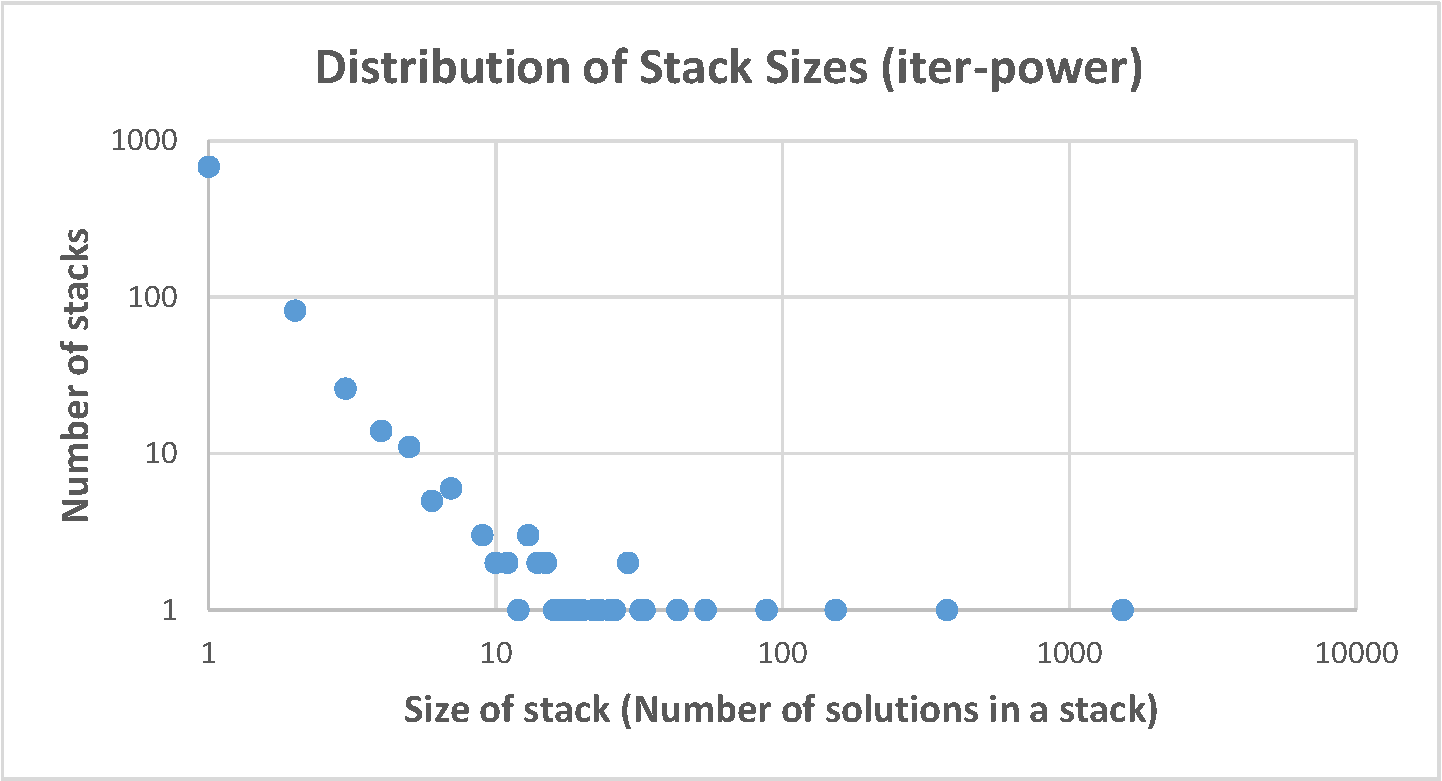
\includegraphics[scale=0.30]{Body/figures/overcode/stacksdistr-iter-power}
&
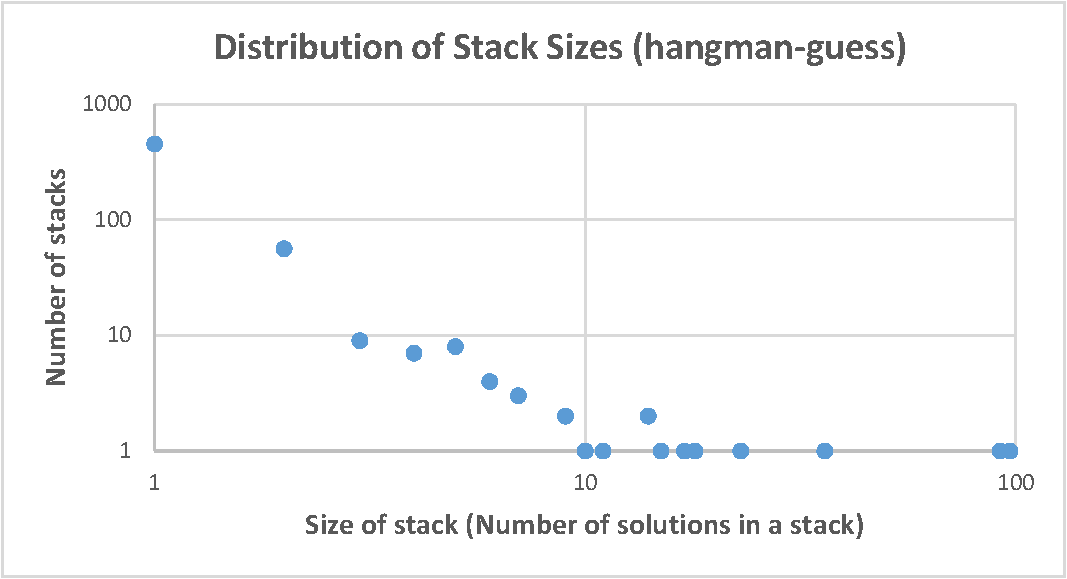
\includegraphics[scale=0.405]{Body/figures/overcode/stacksdistr-hangman}
\end{tabular}
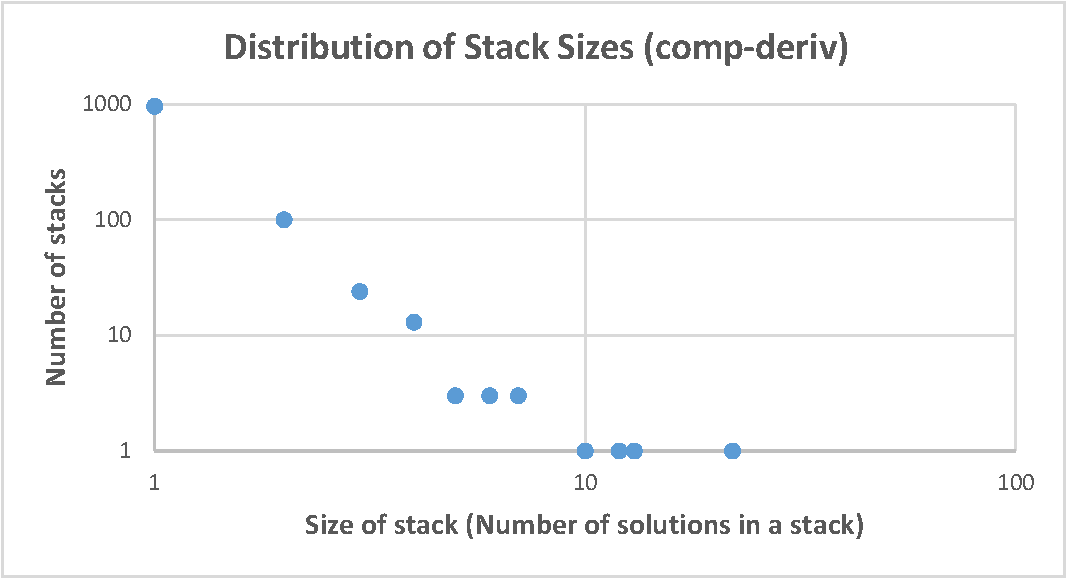
\includegraphics[scale=0.38]{Body/figures/overcode/stacksdistr-comp-deriv}
\caption{The distribution of sizes of the initial stacks generated by our algorithm for each problem, showing a long tail distribution with a few large stacks and a lot of small stacks. Note that the two axes corresponding to the size of stacks and the number of stacks are in logarithmic scale.}
\label{stackdistribution}
\end{figure*}

\begin{figure}[h!]
\begin{tabular}{c}
\\
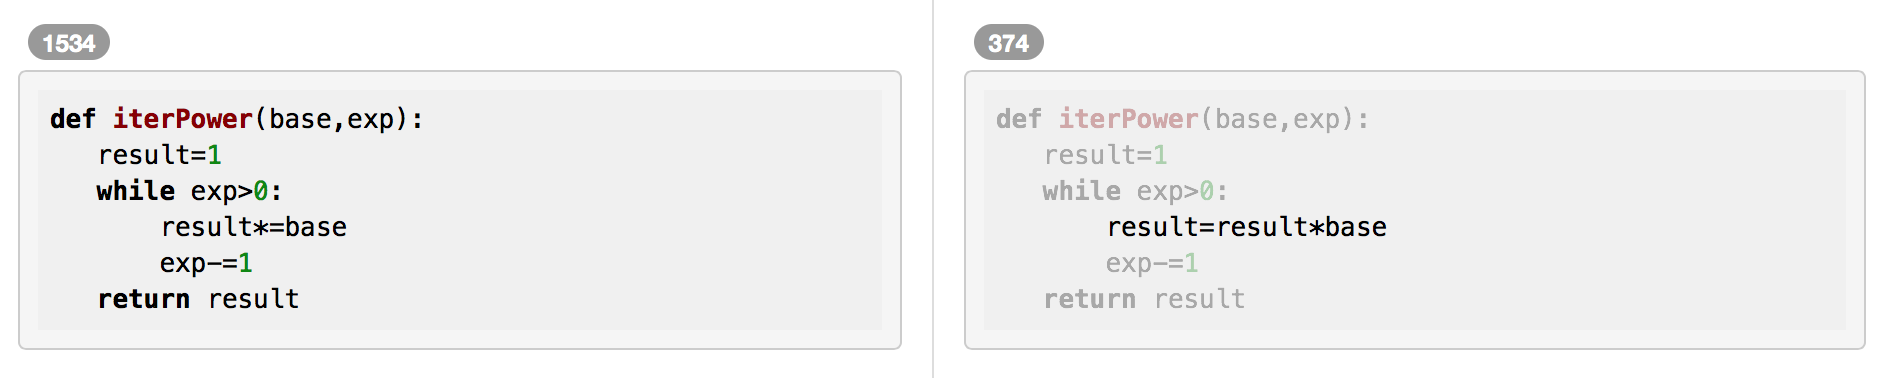
\includegraphics[scale=0.42]{Body/figures/overcode/iterpower-toptwo}
\\ (a) \\ \\
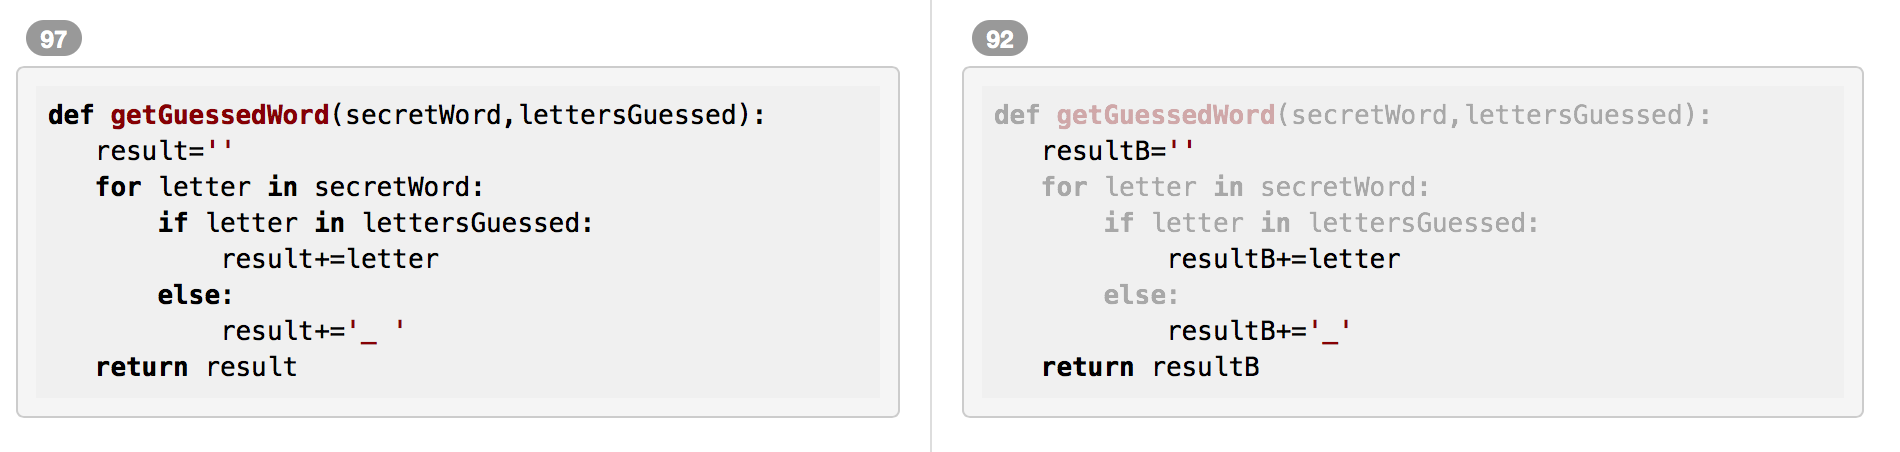
\includegraphics[scale=0.42]{Body/figures/overcode/hangman-toptwo}
\\ (b) \\ \\
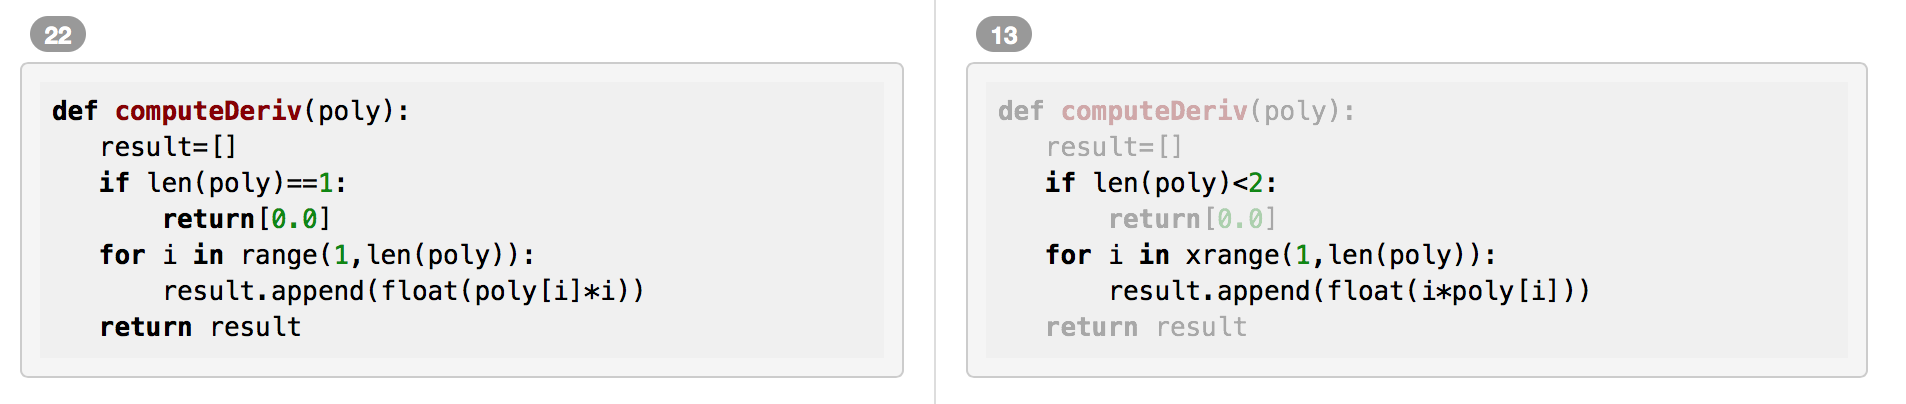
\includegraphics[scale=0.42]{Body/figures/overcode/compderiv-toptwo}
\\ (c) \\
\end{tabular}
\caption{The two largest stacks generated by the OverCode backend algorithm for the (a) \codevar{iterPower}, (b) \codevar{hangman}, and (c)  \codevar{compDeriv} problems.}
\label{toptwostacks}
\end{figure}

{\bf Common Variables} There exists a large variation among the variable names used by students to denote variables that compute the same set of values. The Variable Renaming step of the analysis renames these equivalent variables with the most frequently chosen variable name so that a teacher can easily recognize the role of variables in a given solution. The number of common variables found by the pipeline on the dataset problems is shown in Figure~\ref{backendevaluation} and some examples of these common variable names are shown in Figure~\ref{examplecommonvars}. Figure~\ref{examplecommonvars} also presents the number of times such a variable occurs across the solutions of a given problem, the corresponding variable sequence value on a given test input, and a subset of the original variable names used in the student solutions. 

\begin{figure}
\centering
\scriptsize
\begin{tabular} {|l|r|c|l|}
\hline
{\bf Common} & {\bf Occur} &  \multirow{3}{*}{\bf Sequence of Values} & \multirow{3}{*}{\bf Original Variable Names} \\
{\bf Variable} & {\bf -rence} & & \\
{\bf Name} & {\bf Count} & & \\
 \hline \hline
\multicolumn{4}{|c|}{}\\
\multicolumn{4}{|c|}{\bf iterPower}\\\hline
\codevar{result} & 3081 & [1,5.0,25.0,125.0] & \codevar{result}, \codevar{wynik}, \codevar{out}, \codevar{total}, \codevar{ans}, \codevar{acum}, \codevar{num}, \codevar{mult}, \codevar{output}, $\cdots$\\ \hline
\codevar{exp} & 2744 & [3,2,1,0] & \codevar{exp}, \codevar{iterator}, \codevar{app}, \codevar{ii}, \codevar{num}, \codevar{iterations}, \codevar{times}, \codevar{ctr}, \codevar{b}, $\cdots$\\ \hline
\codevar{exp} & 749 & [3] & \codevar{exp}, \codevar{count}, \codevar{temp}, \codevar{exp3}, \codevar{exp2}, \codevar{exp1}, \codevar{inexp}, \codevar{old\_exp}, $\cdots$\\ \hline
\codevar{i} & 266 & [0,1,2] & \codevar{i}, \codevar{a}, \codevar{count}, \codevar{c}, \codevar{b}, \codevar{iterValue}, \codevar{iter}, \codevar{n}, \codevar{y}, \codevar{inc}, \codevar{x},\codevar{times}, $\cdots$\\ \hline
\multicolumn{4}{|c|}{}\\
\multicolumn{4}{|c|}{\bf hangman}\\\hline
\codevar{letter} & 817 &  [`t',`i',`g',`e',`r'] & \codevar{letter}, \codevar{char}, \codevar{item}, \codevar{i}, \codevar{letS}, \codevar{ch}, \codevar{c}, \codevar{lett}, $\cdots$\\ \hline
\codevar{result} & 291 & [` ',`\_',`\_i',`\_i\_',`\_i\_e',`\_i\_e\_'] & \codevar{result}, \codevar{guessedWord}, \codevar{ans}, \codevar{str1}, \codevar{anss}, \codevar{guessed}, \codevar{string}, $\cdots$\\ \hline
\codevar{i} & 185 & [0,1,2,3,4] & \codevar{i}, \codevar{x}, \codevar{each}, \codevar{b}, \codevar{n}, \codevar{counter}, \codevar{idx}, \codevar{pos} $\cdots$\\ \hline
\codevar{found} & 76 & [0,1,0,1,0] & \codevar{found}, \codevar{n}, \codevar{letterGuessed}, \codevar{contains}, \codevar{k}, \codevar{checker}, \codevar{test}, $\cdots$\\ \hline
\multicolumn{4}{|c|}{}\\
\multicolumn{4}{|c|}{\bf compDeriv}\\ \hline
\codevar{result} & 1186 & [[],[0.0],$\cdots$,[0.0,35.0,9.0,4.0]] & \codevar{result}, \codevar{output}, \codevar{poly\_deriv}, \codevar{res}, \codevar{deriv}, \codevar{resultPoly}, $\cdots$\\ \hline
\codevar{i} & 284 &  [-13.39,0.0,17.5,3.0,1.0] & \codevar{i}, \codevar{each}, \codevar{a}, \codevar{elem}, \codevar{number}, \codevar{value}, \codevar{num}, $\cdots$\\ \hline
\codevar{i} & 261 & [0,1,2,3,4,5] & \codevar{i}, \codevar{power}, \codevar{index}, \codevar{cm}, \codevar{x}, \codevar{count}, \codevar{pwr}, \codevar{counter}, $\cdots$\\ \hline
\codevar{length} & 104 & [5] & \codevar{length}, \codevar{nmax}, \codevar{polyLen}, \codevar{lpoly}, \codevar{lenpoly}, \codevar{z}, \codevar{l}, \codevar{n}, $\cdots$\\ \hline

\end{tabular}
\caption{Some examples of common variables found by our analysis across the problems in the dataset. The table also shows the frequency of occurrence of these variables, the common sequence of values of these variables on a given test case, and a subset of the original variable names used by students.}
\label{examplecommonvars}
\end{figure}

{\bf Collisions in Variable Renaming} The number of Common/Common, Multiple Instances, and Unique/Common collisions discovered and resolved while performing variable renaming is shown in Figure~\ref{collisions}. A large majority of the collisions were Common/Common Collisions. For example, Figure~\ref{examplecommonvars} shows the common variable name \codevar{exp} for two different sequences of values $[3,2,1,0]$ and $[3]$ for the \codevar{iterPower} problem. Similarly, the common variable name \codevar{i} corresponds to sequences $[-13.9, 0.0, 17.5, 3.0, 1.0$ and $[0, 1, 2, 3, 4, 5]$ for the \codevar{compDeriv} problem. There were also a few Multiple Instances collisions and Unique/Common collisions found: 1.5\% for \codevar{iterPower}, 3\% for \codevar{compDeriv}, and 10\% for \codevar{hangman}.

\begin{figure}[htpb]
\centering
\begin{tabular}{|l|r|r|r|r|}
\hline
\multirow{2}{*}{\bf Problem} & {\bf Correct} & {\bf Common/Common} & {\bf Multiple Instances} & {\bf Unique/Common}\\
& {\bf Solutions} & {\bf Collisions } & {\bf Collisions} & {\bf Collisions}\\
\hline \hline
\codevar{iterPower} & 3875 & 1298 & 25 & 32 \\ \hline
\codevar{hangman} & 1118 & 672 & 62 & 49\\ \hline
\codevar{compDeriv} & 1433 & 928 & 21 & 23 \\ \hline
\end{tabular}
\caption{The number of common/common, multiple instances, and unique/common collisions discovered by our algorithm while renaming the variables to common names.}
\label{collisions}
\end{figure}

\section{User Studies}

The goal was to design a system that allows teachers to develop a better understanding of the variation in student solutions, and give feedback that is relevant to more student solutions. Two user studies evaluate our progress in two ways: (1) user interface satisfaction and (2) how many solutions teachers could read and produce feedback on in a fixed amount of time. Reading and providing feedback to thousands of solutions is an unrealistically difficult task for the control condition, so instead of measuring time to finish the entire set of solutions, the experiment measures what subjects could accomplish in a fixed amount of time (15 minutes).

Together, these studies test four hypotheses:
\begin{itemize}
\item \textbf{H1 Interface Satisfaction} Subjects will find OverCode easier to use, more helpful and less overwhelming for browsing thousands of solutions, compared to the baseline. 

\item {\bf H2 Read coverage and speed} Subjects are able to read code that represents more student solutions at a higher rate using OverCode than with the baseline. 

\item {\bf H3 Feedback coverage} Feedback produced when using OverCode is relevant to more student solutions than when feedback is produced using the baseline.

\item {\bf H4 Perceived coverage} Subjects feel that they develop a better high-level view of students' understanding and misconceptions, and provide more relevant feedback using OverCode than with the baseline.

\end{itemize}

\subsection{User Study 1: Writing a Class Forum Post}

The first study was a 12-person within-subjects evaluation of interface satisfaction when using OverCode for a realistic, relatively unstructured task. Using either OverCode or a baseline interface, subjects browse student solutions to the programming problems in our dataset and then write a class forum post on the good and bad ways students solved the problem. This study tests the hypothesis about interface satisfaction (\textbf{H1}).

\subsubsection{OverCode and Baseline Interfaces}

The experiment relies on two interfaces, referred to here as OverCode and the baseline. The OverCode interface and backend are described in detail in Section \ref{overcode}. The baseline interface is a single webpage with all student solutions concatenated in a random order into a flat list, as shown in Figure \ref{iterPowerEdXControl}. This design emulates existing methods of reviewing solutions, and aims to draw out differences between browsing stacked and unstacked solutions. This is analogous to the flat interface chosen as a baseline in another study on interfaces for grading clusters of student work published by Basu et al.~\cite{basuDivideAndConquer}. Basu et al. assume that existing options for reviewing solutions are limited to going through solutions one-by-one. This assumption is supported by our pilot studies, interviews with teaching staff, and our own grading experiences. In edX programming MOOCs, teachers are not even provided with an interface for viewing all solutions at once. They can only look at one student solution at a time. If the solutions can be downloaded locally, some teachers may use a search tool like \codevar{grep}. Our baseline allows for search too, through the in-browser \texttt{Find} command. 

Each solutions is rendered with the same syntax highlighting, background color, and borders in the baseline and OverCode interfaces. However, the solutions shown in the baseline are raw, and the solutions shown in OverCode are normalized. In both interfaces, subjects can use standard web-browser features, such as the within-page \texttt{Find} action.


\begin{figure}[h!]
\centering
\begin{tabular}{cc}
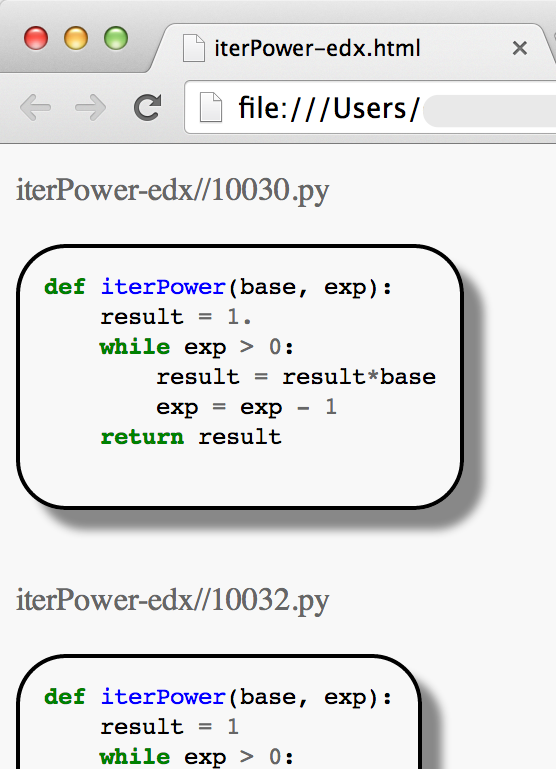
\includegraphics[scale=0.5]{Body/figures/overcode/iterPowerEdXControlStudy1.png} &
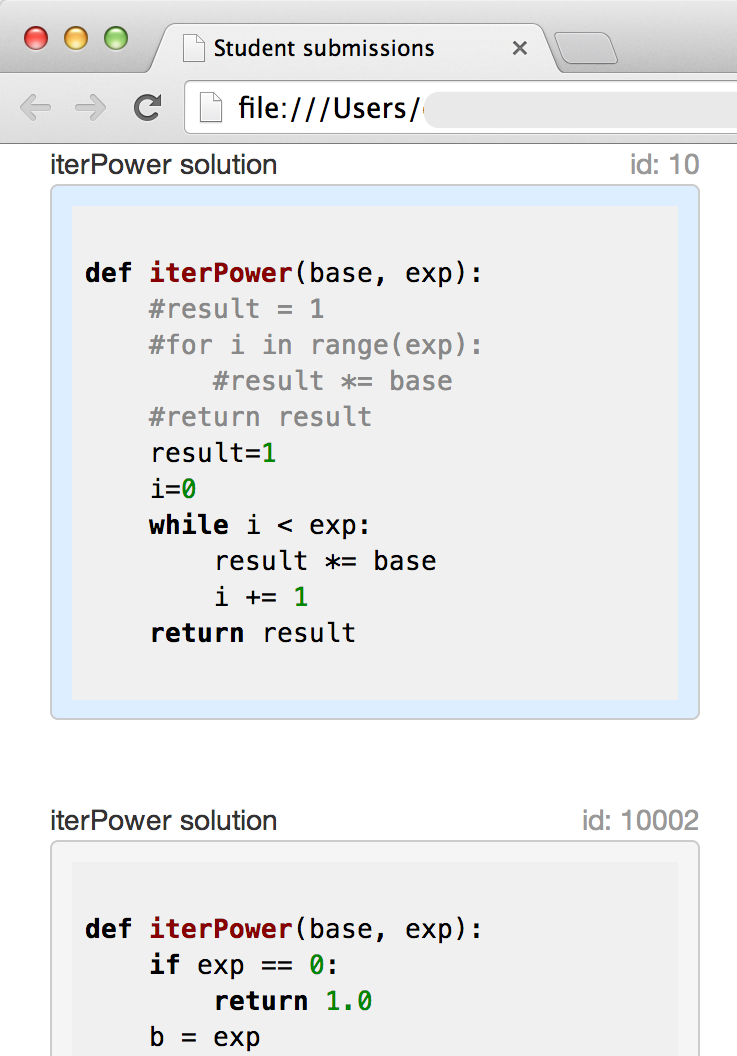
\includegraphics[scale=0.37]{Body/figures/overcode/iterPowerEdXControlStudy2.png} \\
\end{tabular}
\caption{Screenshots of the baseline interface. The appearance changed between the Forum Post study (left) and the Coverage study (right) in order to minimize superficial differences between the baseline and OverCode interfaces. Functionality did not change.}
\label{iterPowerEdXControl}
\end{figure}

\subsubsection{Participants}

Participants joined the study by responding to advertisements sent out to an MIT CSAIL-wide email list as well as past and present staff members of MIT introductory programming courses. These individuals were qualified to participate if they have at least one of the following requirements: (1) taught a computer science course (2) graded Python code before, or (3) significant Python programming experience, making them potential future teaching staff. Participants received \$20 for an hour of their time in the lab. 

Subjects filled out forms about themselves during recruitment and again at the beginning of their one-hour in-lab session. 12 people (7 male) participated, with a mean age of 23.5 ($\sigma = 3.8$). Subjects had a mean 4 years of Python programming experience ($\sigma = 1.8$), and $75\%$ of participants had graded student solutions written in Python before. Half of the participants were graduate students and the other half were undergraduates.

\subsubsection{Apparatus}

Subjects used laptops running MacOS and Linux with screen sizes ranging from 12.5 to 15.6 inches, and viewed the OverCode and baseline interfaces in either Safari or Chrome. Data was recorded with Google Docs and Google Forms filled out by participants.

\subsubsection{Conditions}

Subjects performed the main task of browsing solutions and writing a class forum post twice, once in each interface condition, focusing on one of the three problems in our dataset (Section \ref{dataset}) each time. For each participant, the third remaining problem was used during training, to reduce learning effects when performing the two main tasks. The pairing and ordering of interface and problem conditions were fully counterbalanced, resulting in 12 total conditions. The twelve participants were randomly assigned to one of the 12 conditions, such that all conditions were tested.

\subsubsection{Procedure}

{\bf Prompt} The experimenter began by reading the following prompt, to give the participant context for the tasks they would be performing:

\begin{quote}

We want to help TAs [teaching assistants] give feedback to students in programming classes at scale. For each of three problems, we have a large set of students' submissions ($> 1000$). 

All the submissions are correct, in terms of input and output behavior. We're going to ask you to browse the submissions and produce feedback for students in the class. You'll do this primarily in the form of a class forum post.
\end{quote}

To make the task more concrete, participants reviewed an example\footnote{Our example was drawn from the blog ``Practice Python: 30-minute weekly Python exercises for beginners,'' posted on Thursday, April 24, 2014, and titled ``SOLUTION Exercise 11: Check Primality and Functions.'' (\url{http://practicepython.blogspot.com})} of a class forum post that used examples taken from student solutions to explain different strategies for solving a Python problem. For reference, subjects had print-outs of the prompts for each of the three problems in our dataset.

{\bf Training} The subjects already had extensive experience using web browsers, so training for the baseline interface was minimal. Prior to using the OverCode interface, subjects watched a 3-4 minute long training video demonstrating the features of OverCode, familiarized themselves with the interface, and asked questions. The training session focused on the problem that would not be used in the main tasks, in order to avoid learning effects.

{\bf Tasks} Subjects then performed the main tasks twice, once in each interface, focusing on a different programming problem each time. They were given a fixed amount of time to both read solutions and provide feedback, so task completion times were not measured, but instead the quality of their experience in providing feedback to students at scale.

\begin{itemize}
\item {\it Feedback for Students} (15 minutes) Subjects wrote a class forum post on the good and bad ways students solved the problem. The 15-minute period included both browsing and writing time, as subjects were free to paste in code examples and write comments as they browsed the solutions.

\item {\it Autograder Bugs} (2 min) Although the datasets of student solutions were marked as correct by an autograder, there may be holes in the autograder test cases. Some solutions may deviate from the problem prompt, and therefore be considered incorrect by teachers, e.g., recursive solutions to \codevar{iterPower} when its prompt explicitly calls for an iterative solution. As a secondary task, subjects wrote down any bugs in the autograder they came across while browsing solutions. This was often performed concurrently with the primary task by the subject.
\end{itemize}
{\bf Surveys} Subjects filled out a post-interface condition survey about their experience using the interface. This was a short-answer survey, where they wrote about what they liked, what they did not like, and what they would like to see in a future version of the interface. At the end of the study, subjects rated agreement (on a 7-point Likert scale) with statements about their satisfaction with each interface.

\subsubsection{Results}
Figure~\ref{study1Likert} shows that, compared to the control interface, subjects find OverCode less overwhelming, easier to use, and more helpful for getting a sense of students' understanding. After using both interfaces to view thousands of solutions, subjects found OverCode easier to use ($W=52, Z=2.41, p<0.05, r=0.70$) and less overwhelming ($W=0, Z=-2.86, p<0.005, r=0.83$) than the baseline interface. Finally, participants felt that OverCode ``helped me get a better sense of my students' understanding'' than the baseline did ($W=66, Z=3.04, p<0.001, r=0.88$). These differences are statistically significant, as computed by the Wilcoxon Signed Rank test with pairing users' ratings of each interface. This supports \textbf{H1}, the hypothesis on interface satisfaction.

\begin{figure}
\centering
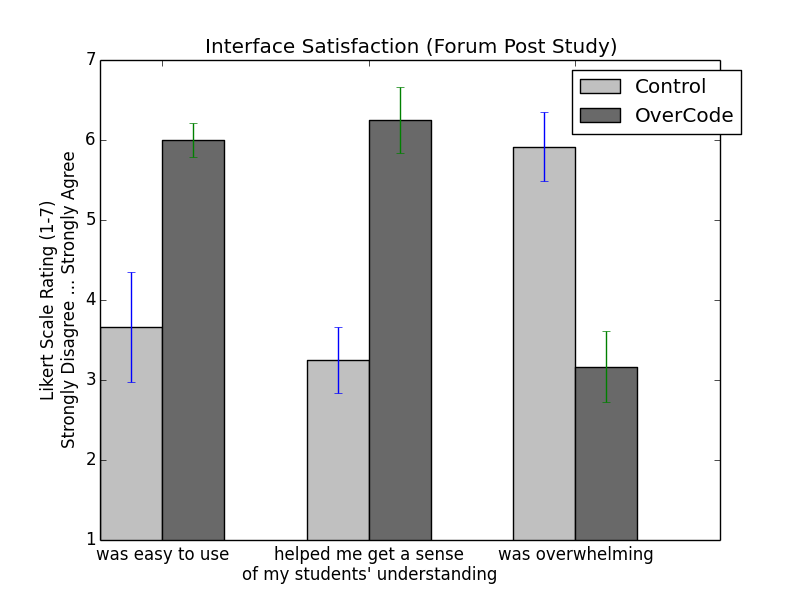
\includegraphics[scale=0.5]{Body/figures/overcode/study1Likert.png}
\caption{{\bf H1: Interface satisfaction} Mean Likert scale ratings (with standard error) for OverCode and baseline interfaces, after subjects used both to perform the forum post writing task.}
\label{study1Likert}
\end{figure}


From the surveys conducted after subjects completed each interface condition, subjects found stacking and the ability to rewrite code to be useful and enjoyable features of OverCode:
\begin{itemize}
\item {\it Stacking is an awesome feature. Rewrite tool is fantastic. Done feature is very rewarding--feels much less overwhelming. "Lines that appear in x submissions" also awesome.}

\item {\it Really liked the clever approach for variable normalization. Also liked the fact that stacks showed numbers, so I'd know I'm focusing on the highest-impact submissions. Impressed by the rewrite ability... it cut down on work so much!}

\item {\it I liked having solutions collapsed (not having to deal with variable names, etc), and having rules to allow me to collapse even further. This made it easy to see the ``plurality'' of solutions right away; I spent most of the time looking at the solutions that only had a few instances.}
\end{itemize}

When asked for suggestions, participants gave many suggestions on stacks, filtering, and rewrite rules, such as:
\begin{itemize}
\item Enable the teacher to change the main stack that is being compared against the others.
\item Suggest possible rewrite rules, based on what the teacher has already written, and will not affect the answers on the test case.
\item Create a filter that shows all stacks that do {\it not} have a particular statement.
\end{itemize}

For both the OverCode and baseline interfaces, the feedback generated about \codevar{iterPower}, \codevar{hangman}, and \codevar{compDeriv} solutions fell into several common themes. One kind of feedback suggested new language features, such as using \codevar{*=} or the keyword \codevar{in}. Another theme identified inefficient, redundant, and convoluted control flow, such as repeated statements and unnecessary statements and variables. It was not always clear what the misconception was, though, as one participant wrote, \textit{``The double iterator solution surely shows some lack of grasp of power of for loop, or range, or something.''} Participant feedback included comments on the relative goodness of different correct solutions in the dataset. This was a more holistic look at student solutions as they varied along the dimensions of conciseness, clarity, and efficiency previously described.

Study participants found both noteworthy correct solutions and solutions they considered incorrect, despite passing the autograder. One participant learned a new Python function, \codevar{enumerate}, while looking at a solution that used it. The participant wrote, \textit{``Cool, but uncalled for. I had to look it up :]. Use, but with comment.''} Participants also found recursive \codevar{iterPower} and \codevar{hangman} solutions, which they found noteworthy. For what should have been an iterative \codevar{iterPower} function, the fact that this recursive solution was considered correct by the autograder was considered an autograder bug by some participants. Using the built-in Python exponentiation operator \codevar{**} was also considered correct by the autograder, even though it subverted the point of the assignment. It was also noted as an autograder bug by some participants who found it.

\subsection{User Study 2: Coverage}

A second 12-person study was designed, similar in structure to the forum post study, but focused on measuring the coverage achieved by subjects in a fixed amount of time (15 minutes) when browsing and producing feedback on a large number of student solutions. The task in the second study was more constrained than the first. Instead of writing a freeform post, subjects identified the five most frequent strategies used by students and rated their confidence that these strategies occurred frequently in the student solutions. These changes to the task enabled us to measure coverage in terms of solutions read, the relevance of written feedback and the perceived coverage of the subject. This study tests the remaining hypotheses on read coverage and speed ({\bf H2}), feedback coverage ({\bf H3}) and perceived coverage ({\bf H4}).

The OverCode and baseline interfaces changed slightly prior to running the second study. Figure \ref{iterPowerEdXControl} shows the baseline changes that reduce the differences between the rendering of solutions in the baseline and OverCode interfaces. The OverCode interface was changed to show identifiers next to every stack and solutions so that subjects could provide it when asked.

\subsubsection{Participants, Apparatus, Conditions}

The coverage study shared the same methods for recruiting participants, apparatus and conditions as the forum post study. 12 new participants (11 male) participated in the second study (mean age = 25.4, $\sigma = 6.9$). Across those 12 participants, the mean years of Python programming experience was 4.9 ($\sigma = 3.0$) and 9 of them had previously graded code (5 had graded Python code). Subjects included 5 graduate students, 6 undergraduates, and 1 independent computer software professional.


\subsubsection{Procedure}
{\bf Prompt} In the coverage study, the prompt was similar to the one used in the forum post study, explaining that the subjects would be tackling the problem of producing feedback for students at scale. The language was modified to shift the focus towards finding frequent strategies used by students, rather than any example of good or bad code used by a student.%\todo{find prompt and put it in here}

{\bf Training} As before, subjects watched a training video and given time to practice using OverCode features prior to their trial in the OverCode condition.

{\bf Task} The coverage study task consisted of a more constrained feedback task. Given 15 minutes with either the OverCode or baseline interface, subjects filled out a table, identifying the five most frequent strategies used by students to solve the problem. For each strategy they identified, they filled in the following fields in the table:
\begin{itemize}
\item A code example taken from the solution or stack.
\item The identifier of the solution or stack.
\item A short (one sentence) annotation of what was good or bad about the strategy.
\item Their confidence, on a scale of 1-7, that the strategy frequently occurred in the student solutions.
\end{itemize}
Importantly, subjects marked solutions or stacks as \emph{read} by clicking on them after they had processed them, even if they did not choose them as representative strategies. We combined this data with logs of subject actions in the interface to quantify read coverage.

{\bf Surveys} Although we measured interface satisfaction for a realistic task in the forum post study, we also measured interface satisfaction through surveys for this more constrained, coverage-focused task. Subjects filled out a post-interface condition survey in which they rated agreement (on a 7-point Likert scale) with positive and negative adjectives about their experience using the interface, and reflected on task difficulty. At the end of the study, subjects rated their agreement with statements about the usefulness of specific features of both the OverCode and baseline interfaces, and responded to the same interface satisfaction 7-point Likert scale statements used in the first study.

\subsubsection{Results} \label{coverageResults}
\begin{figure*}[b!]
\begin{tabular}{c | c}
\begin{minipage}{.5\linewidth}
\centering
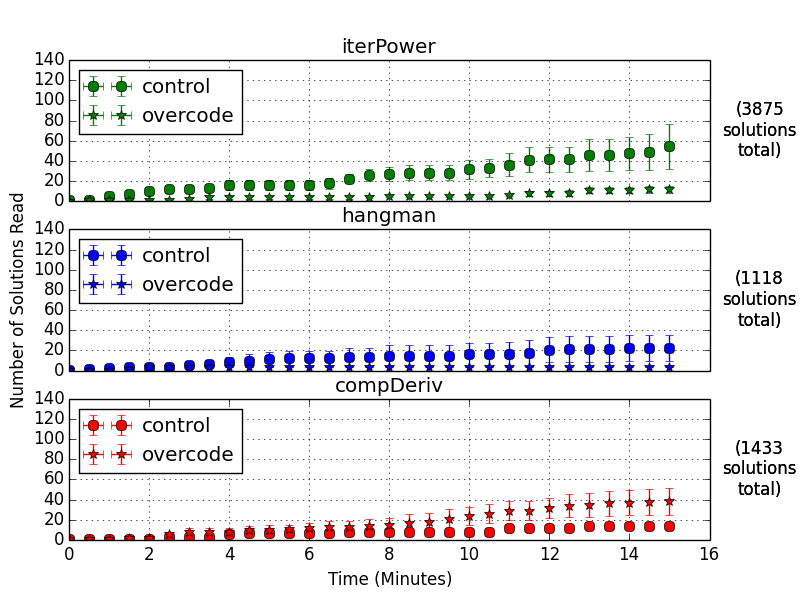
\includegraphics[width=\linewidth]{Body/figures/overcode/prettyReadCoverage.png}
\end{minipage}
&
\begin{minipage}{.5\linewidth}
\centering
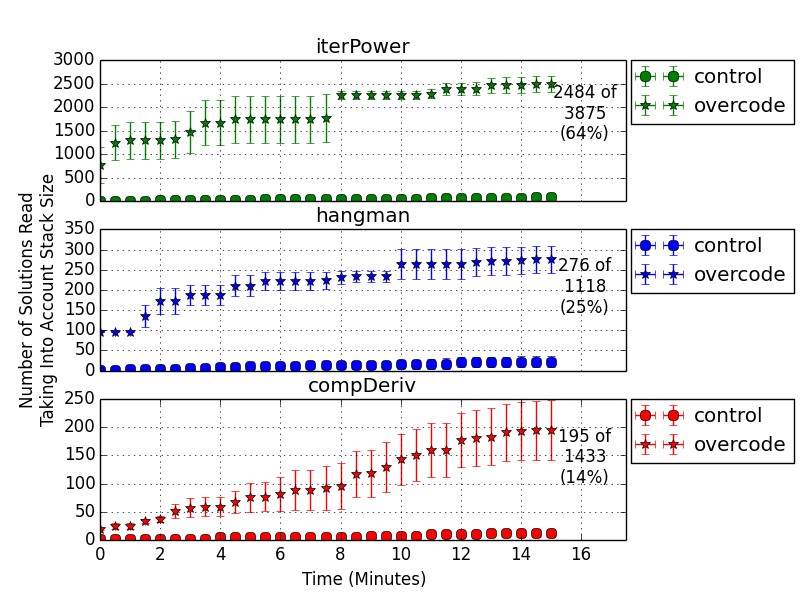
\includegraphics[width=\linewidth]{Body/figures/overcode/prettyPercentCoverage.png}
\end{minipage}
\\
(a) & (b)
\end{tabular}
\caption{In (a), we plot the mean number of platonic solutions read in OverCode over time versus the number of raw solutions read in the baseline interface over time while performing the 15-minute Coverage Study task. In (b), we replace the mean number of platonic solutions with the mean number of solutions, i.e., the stack size, they represent. These are shown for each of the three problems in the dataset.}
\label{readCoverage}
\end{figure*}

{\bf H2: Read coverage and speed} Figure \ref{readCoverage} shows that subjects reading platonic \texttt{iterPower}, \texttt{hangman}, and \texttt{compDeriv} solutions in the OverCode interface covered the equivalent of 64\%, 25\%, and 14\% of all student solutions to those problems (Mann--Whitney U = 16, n1 = n2 = 4, p<0.05). Subjects read through more raw solutions than platonic solutions to the simplest problems, i.e., \texttt{iterPower} and \texttt{hangman}, but when problem difficulty increased, i.e., \texttt{compDeriv}, subjects read through the platonic solutions in the OverCode interface faster than raw solutions. This supports the H2 hypothesis.

%This hypothesis is supported by our measurements of read coverage from this study. For each problem, subjects were able to view more normalized and stacked solutions by the end of the 15-minute-long main task using OverCode than raw solutions when using the baseline interface (Mann--Whitney U = 16, n1 = n2 = 4, p<0.05). Figure \ref{readCoverage} shows the mean number of solutions read over time for each interface and each problem in our dataset. The curves show that subjects were able to read code that represented more raw solutions at a higher rate due to the stacking of similar solutions.

{\bf H3: Feedback coverage} Each subject reported on the five most frequent strategies in a set of solutions, by copying both a code example and the identifier of the solution (baseline) or stack (OverCode) that it came from. We define \emph{feedback coverage} as the number of students for which the quoted code is relevant, in the sense that they wrote the same lines of code, ignoring differences in whitespace or variable names. We computed the coverage for each example using the following process:
\begin{itemize}
\item Reduce the quoted code down to only the lines referred to in the annotation. Often, the annotation would focus on a specific feature of the quoted code, which sometimes included additional lines unrelated to the written feedback. For example, comments about iterating over a range function, while also quoting the contents of the for loop. This step meant we would be calculating the coverage of a more general, smaller set of lines.

\item Find the source stack that the quoted code comes from. This is trivial in the OverCode condition, where the subject wrote down a stack ID. In the baseline condition, the subject wrote down the solution ID. During post-study analysis, the authors determined which stack the solution is in, as determined by the OverCode analysis pipeline.

\item Find the normalized version of each quoted line. The quoted lines of code may be raw code if they come from the baseline condition. By comparing the quoted code with the normalized code of its source stack, we found the normalized version of each line, with variable names and whitespace normalized.

\item Find the raw solutions that include the set of normalized lines, using a map from stacks to raw solutions provided by the backend pipeline.
\end{itemize}

\begin{figure}[b!]
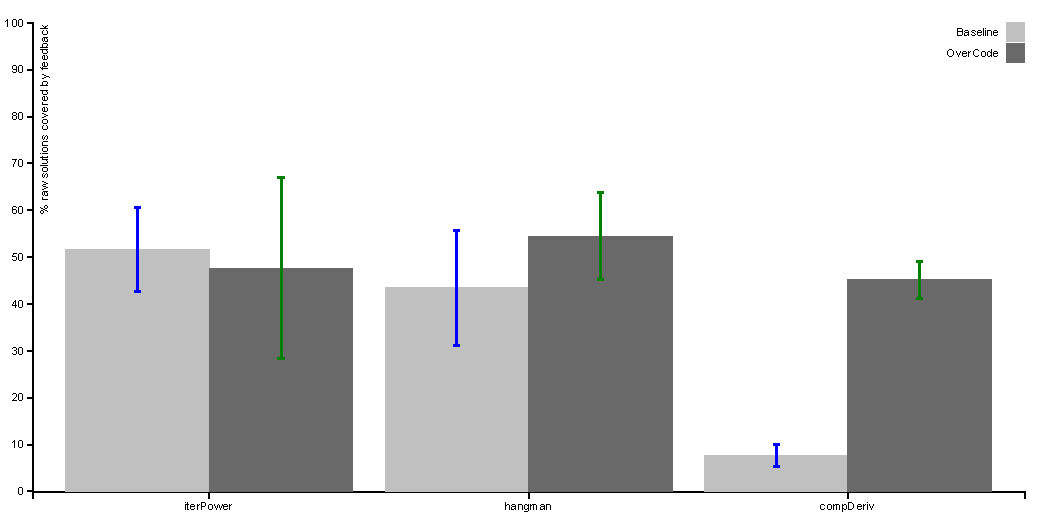
\includegraphics[width=0.6\paperwidth]{Body/figures/overcode/feedbackCoverage.pdf}
\caption{Mean feedback coverage, i.e., the percentage of raw solutions covered, per trial during the coverage study for each problem, in the OverCode and baseline interfaces.}
\label{aveCoveragePerPost}
\end{figure}
%\todo{DNHT: what are the error bars?}

Figure \ref{aveCoveragePerPost} shows the mean coverage of a set of feedback produced by a single subject, across problems and interface conditions. The feedback coverage is shown as the mean percentage of raw solutions for which the feedback was relevant. When giving feedback on the \codevar{iterPower} and \codevar{hangman} problems, there was not a statistically significant difference in the feedback coverage between interface conditions. However, on \codevar{compDeriv}, the problem with the most complex solutions, subjects using OverCode achieved significantly more coverage of student solutions than when using the baseline interface (Mann--Whitney U = 0, n1 = n2 = 4, p< 0.05).

\begin{figure*}[t!]
\begin{tabular}{c | c}
\begin{minipage}{.5\linewidth}
\centering
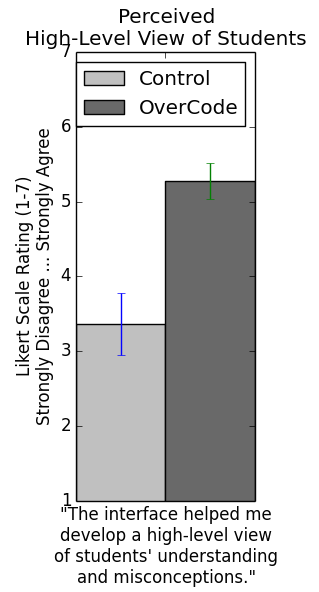
\includegraphics[scale=0.5]{Body/figures/overcode/highLevelViewStudy2.png}
\end{minipage}
&
\begin{minipage}{.5\linewidth}
\centering
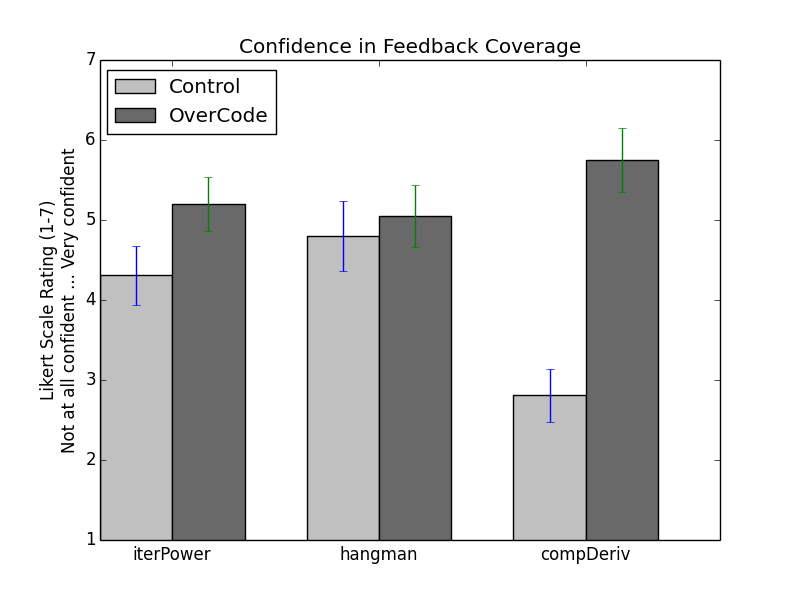
\includegraphics[width=\linewidth]{Body/figures/overcode/coverageConfidence.png}
\end{minipage}
\\
(a) & (b)
\end{tabular}
\caption{Mean rating with standard error for (a) post-condition perception of coverage (excluding one participant) and (b) confidence ratings that identified strategies were frequently used (1-7 scale).}
\label{perceivedCoverage}
\end{figure*}

{\bf H4: Perceived coverage} After using each interface, we asked participants how strongly they agreed with the statement `This interface helped me develop a high-level view of students' understanding and misconceptions,' which quotes the first part of our third hypothesis. Participants agreed with this statement after using OverCode significantly more than when using the baseline interface ($W=63, Z=2.70, p<0.01, r=0.81$). Statistical significance was computed using the Wilcoxon Signed Rank test, pairing users' ratings of each interface. The analysis was done for only 11 participants because the data of one participant was lost. The mean rating with standard error for the responses is shown in Figure~\ref{perceivedCoverage}(a). 

For each strategy identified by subjects, we asked them to rate their confidence, on a scale of 1-7, that the strategy was frequently used by students in the dataset. Mean confidence ratings on a per-problem basis are shown in Figure \ref{perceivedCoverage}(b). We found that for \codevar{compDeriv}, subjects using OverCode felt significantly more confident that their annotations were relevant to many students, compared to the baseline (Mann--Whitney $U=260.5, n_{1}=18, n_{2}=16, p<0.0001$).
 
{\bf H1: Interface satisfaction} Interface satisfaction was measured through multiple surveys, (1) immediately after using each interface and (2) after using both interfaces. Statistical significance was computed using the Wilcoxon Signed Rank test, pairing users' ratings of each interface. 

Immediately after finishing the assigned tasks with an interface, participants rated their agreement with statements about the appropriateness of various adjectives to describe the interface they just used, on a 7-point Likert scale. While participants found the baseline to be significantly more simple ($W=2.5, Z=-2.60, p<0.01, r=0.78$), they found OverCode to be significantly more flexible ($W=45, Z=2.84, p<0.005, r=0.86$), less tedious ($W=3.5, Z=-2.41, p<0.05, r=0.73$), more interesting ($W=66, Z=2.96, p<0.001, r=0.89$), and more enjoyable ($W=45, Z=2.83, p<0.005, r=0.85$). The analysis was done for only 11 participants because the data of one participant was lost. The mean ratings (with standard error) for the responses are shown in Figure~\ref{studyLikert1_onPop2}. 

After the completion of the Coverage Study, participants rated their agreement with statements about each interface on a 7-point Likert scale. After using both interfaces to view thousands of solutions, there were no significant differences between how overwhelming or easy to use each interface was. However, participants did feel that OverCode ``helped me get a sense of my students' understanding'' more than the baseline ($W=62.5, Z=-2.69, p<0.01, r=0.78$). The mean ratings for the responses are shown in Figure~\ref{studyLikert1_onPop2}, as well as the standard error.

\begin{figure}
\centering
\begin{tabular}{c c}
\begin{minipage}{.6\linewidth}
\centering
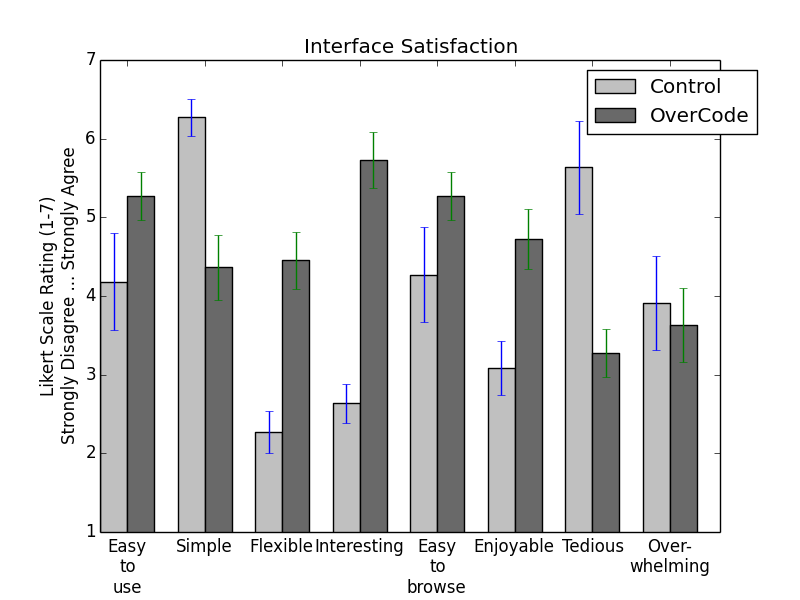
\includegraphics[scale=0.35]{Body/figures/overcode/study2Likert.png}
\end{minipage}
&
\begin{minipage}{.4\linewidth}
\centering
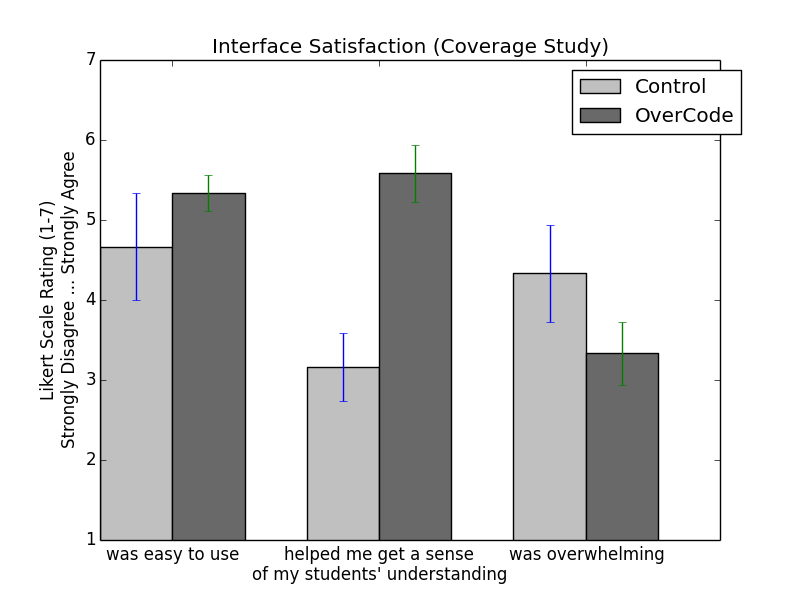
\includegraphics[scale=0.30]{Body/figures/overcode/study1Likert_onPop2.png}
\end{minipage}
\\
(a) & (b)
\end{tabular}
\caption{{\bf H1: Interface satisfaction} Mean Likert scale ratings (with standard error) for  OverCode and baseline, (a) immediately after using the interface for the Coverage Study task, and (b) after using both interfaces.}
\label{studyLikert1_onPop2}
\end{figure}

{\bf Usage and Usefulness of Interface Features} In the second part of the post-study survey, participants rated their agreement with statements about the helpfulness of various interface features on a 7-point Likert scale. There were only two features to ask about in the baseline interface, in-browser find and viewing raw solutions. Statements about these baseline features were mixed in with statements about OverCode features. The OverCode feature of stacking equivalent solutions was found more helpful than the baseline features of in-browser find ($W=41, Z=2.07, p<0.05, r=0.60$) and viewing raw student solutions, comments included ($W=45, Z=2.87, p<0.005, r=0.83$). Subjects found both the OverCode feature of variable renaming and previewing rewrite rules significantly more helpful than seeing raw student code ($W=65.5, Z=2.09, p<0.05, r=0.61$ and $W=56.5, Z=2.14, p<0.05, r=0.62$, respectively). The mean ratings for the features are shown in Figure~\ref{featureHelpfulness}.

\begin{figure}
\centering
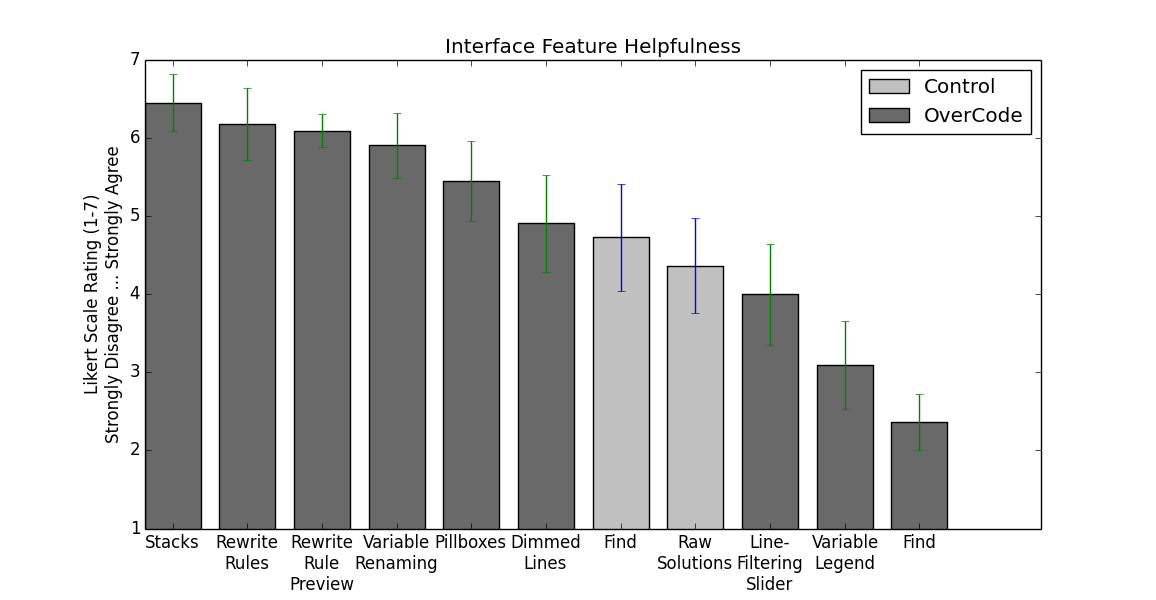
\includegraphics[scale=0.5]{Body/figures/overcode/featureHelpfulness.png}
\caption{Mean Likert scale ratings (with standard error) for the usefulness of features of OverCode and baseline. {\it Find} refers to the find function within the web browser. {\it Find} appears twice in this figure because users rated its usefulness for each condition.}
\label{featureHelpfulness}
\end{figure}

In addition to logging \codevar{read} events, we also recorded usage of interface features, such as creating rewrite rules and filtering stacks. A common usage strategy was to read through the stacks linearly and mark them as \codevar{read}, starting with the largest reference stack, then rewrite trivial variations in expressions to merge smaller behaviorally equivalent stacks into the largest stack. Stack filtering (Figure~\ref{linefilter}) was sometimes used to review solutions that contained a particularly conspicuous line, e.g., a recursive call to solve \codevar{iterPower} or an extremely long expression. Subjects rarely used the filter panel frequency slider (Figure~\ref{linefilter}a) and the variable legend (Figure~\ref{afterrewrite}b).

All subjects wrote at least two rewrite rules, often causing stacks to merge that only differed in some trivial way, like reordering operands in multiplication statements, e.g., \codevar{result = result*base} vs. \codevar{result = base*result}. Some rewrite rules merged Python expressions that behaved similarly but differed in their verbosity, e.g., \codevar{for i in range(0, exp)} vs. \codevar{for i in range(exp)}. These variations may be considered noteworthy or trivial by different teachers.

\section{Discussion}

A three-part evaluation of the OverCode backend and user interface demonstrates its usability and usefulness in a realistic teaching scenario. Given that the datasets are drawn from the first three weeks of an introductory Python programming course, the evaluation is limited to single functions, whose most common solutions were less than ten lines long. Some of these functions were recursive, while most were iterative. Variables were generally limited to booleans, integers, strings, and lists of these basic data types. All solutions had already passed the autograder tests, and study participants still found solutions that suggested student misconceptions or knowledge gaps. Future work will address more complex algorithms and data types.

\subsubsection{Read coverage}
Subjects covered more student solutions when reading solutions in the OverCode interface (H1, read coverage). This is expected, because in OverCode each read stack represented tens or hundreds of raw solutions, while there was only a 1-to-1 mapping between read solutions and raw solutions in the baseline condition. The OverCode backend produces platonic solutions that represent many raw solutions, reducing the cognitive load of mentally processing all the raw solutions, including their variation in formatting and variable naming.

Figure \ref{readCoverage}(a) shows that in some cases, subjects read nearly as many (\codevar{hangman}) or more (\codevar{iterPower}) function definitions in the baseline as in OverCode. In the case of \codevar{iterPower}, the raw solutions are repetitive because of the simplicity of the problem and the relatively small amounts of variation demonstrated by student solutions. This can explain the ability of subjects to move quickly through the set of solutions, reading as many as 90 solutions in 15 minutes.

Figure \ref{readCoverage}(b) shows the effective number of raw solutions read, when accounting for the number of solutions represented by each platonic solution read in the OverCode condition. In the case of \codevar{iterPower}, subjects can say they have effectively read more than 30\% of student solutions after reading the first stack. A similar statement can be made for \codevar{hangman}, where the largest stack includes roughly 10\% of solutions. In the case of \codevar{compDeriv}, the small size of its largest stack (22 out of 1433 raw solutions) means that the curve is less steep, but the use of rewrite rules (avg. 4.5 rules written per \codevar{compDeriv} subject) enabled subjects to cover over 10x the solutions covered by subjects in the baseline condition.

\subsubsection{Feedback coverage}
We also found that subject-written feedback on solutions for the \codevar{compDeriv} problem had significantly higher coverage when produced using OverCode than with the baseline, but that this was not the case for the \codevar{iterPower} and \codevar{hangman} problems. \codevar{compDeriv} was a significantly more complicated problem than both \codevar{iterPower} and \codevar{hangman}, meaning that there was a greater amount of variation between student solutions. This high variation meant that any one piece of feedback might not be relevant to many raw solutions, unless it was produced after viewing the solution space as stacks and creating rewrite rules to simplify the space into larger, more representative stacks. Conversely, the simple nature of \codevar{iterPower} and \codevar{hangman} meant that there was less variation in student solutions. Therefore, regardless of whether the subject was using the OverCode or baseline condition, there was a higher likelihood that they would stumble across a solution that had frequently occurring lines of code, and the feedback coverage for these problems became comparable between the two problems.

\subsubsection{Perceived coverage}
In addition to the actual read and feedback coverage that subjects achieved, an important finding was that (i) subjects felt they had developed a better high-level understanding of student solutions and (ii) subjects stated they felt more confident that identified strategies were frequent issues in the dataset. While a low self-reported confidence score did not necessarily correlate with low feedback coverage, these results suggest that OverCode enables the teacher to gauge the impact that their feedback will have.

%\section{Modifications and Extensions}

%\subsection{Handling Multiple Test Cases}
%For the convenience and speed of adding more solutions without unnecessary repeated computation,

%\subsection{Multiple Test Cases and Efficiency} 
%Since publication, the OverCode pipeline has been modified in several ways. 
%\subsection{Collecting Additional Information per Line}~\label{subsec:morelineinfo}
%, as described in Section~\ref{subsec:grovercodepipeline}.
% is, without being affected a very similar concept, except it is more robust to non-local variations in variable behavior. For example, if the line of code \texttt{for ___ in range(___):}initialization of two common variables 

\subsubsection{Clarity in Variable Renaming}
The modifiers appended to common variables to resolve Common/Common collisions caused some confusion. For example, \texttt{iB} is a legitimate, but odd, variable name. To indicate that the modifier is not something the student wrote themselves, modifiers are now rendered in the interface as numerical subscripts indicating whether they are the second or third or fourth, etc., most frequently occurring common variable with that name across all the solutions in the collection.

\section{GroverCode: OverCode for Grading}\label{sec:grover}

While understanding the contents of thousands of correct student solutions can be helpful in both residential and online contexts, another application of the OverCode pipeline and interface is supporting the hand-grading of introductory Python programming exam solutions, only some of which are correct. Incorrect solutions are defined as those that do not pass at least one test case in the teacher-designed test suite.

Hand-reviewing solutions is necessary because test suites can unfairly penalize some students and award undeserved credit to others. For example, a single typo in an otherwise well-written solution can cause it to fail all the test cases and receive no credit. Conversely, a solution that subverts the purpose of the assignment can still receive credit by returning the expected answer to some or all of the test cases.

For the staff of 6.0001, the residential introductory Python programming course at MIT, this can be one of the most time-consuming and exhausting parts of teaching the course. It can take a full workday for the entire staff of eight to ten teachers to sit in a room and review several hundred student solutions by hand in order to assign a single numerical grade to each solution.

Stacey Terman, in partial fulfilment of her Master's of Engineering, worked with me to extend OverCode to a new domain, i.e., incorrect solutions, and a new task, i.e., grading hundreds of incorrect solutions by hand~\cite{staceythesis}. This new version of OverCode for grading is referred to as GroverCode. GroverCode was iteratively designed and evaluated as a grading tool through two live deployments during the Spring 2016 6.0001 staff exam grading sessions. The following tables, figures, and code samples generated from those deployments are adapted with permission from that thesis.

GroverCode contains two main technical contributions: a modified pipeline that can normalize both correct and incorrect solutions and an interface designed for grading. Just as the original pipeline used variable behavior to normalize variable names, the modified pipeline uses variable behavior and the syntax of statements containing each variable to normalize variable names in solutions that are not correct. This comes from the insight that a variable in an incorrect solution can be semantically equivalent to a variable in a correct solution but still behave differently. It can behave differently due to a bug in a line of code that directly modifies its value or a bug in a line of code that affects the behavior of another variable that it depends on. Since many of the exam solutions are incorrect and do not get clustered together, the new user interface organizes solutions according to their behavior on test cases and compositional similarity to each other, rather than by cluster size.

\subsubsection{User Interface}

The GroverCode interface, shown in Figure~\ref{fig:whole_interface}, has several additions and distinctions from the OverCode interface. As shown in Figure~\ref{fig:correct_and_incorrect_stacks}, both correct solutions and incorrect solutions are displayed, differentiable by their varied background colors and red X next to every failed test. To better explain each test failure, the actual and expected outputs are displayed beneath each solution. The staff iteratively develop a rubric as they grade. Figure~\ref{fig:rubric} is a snapshot of one of these rubrics.

\begin{figure}
\centering
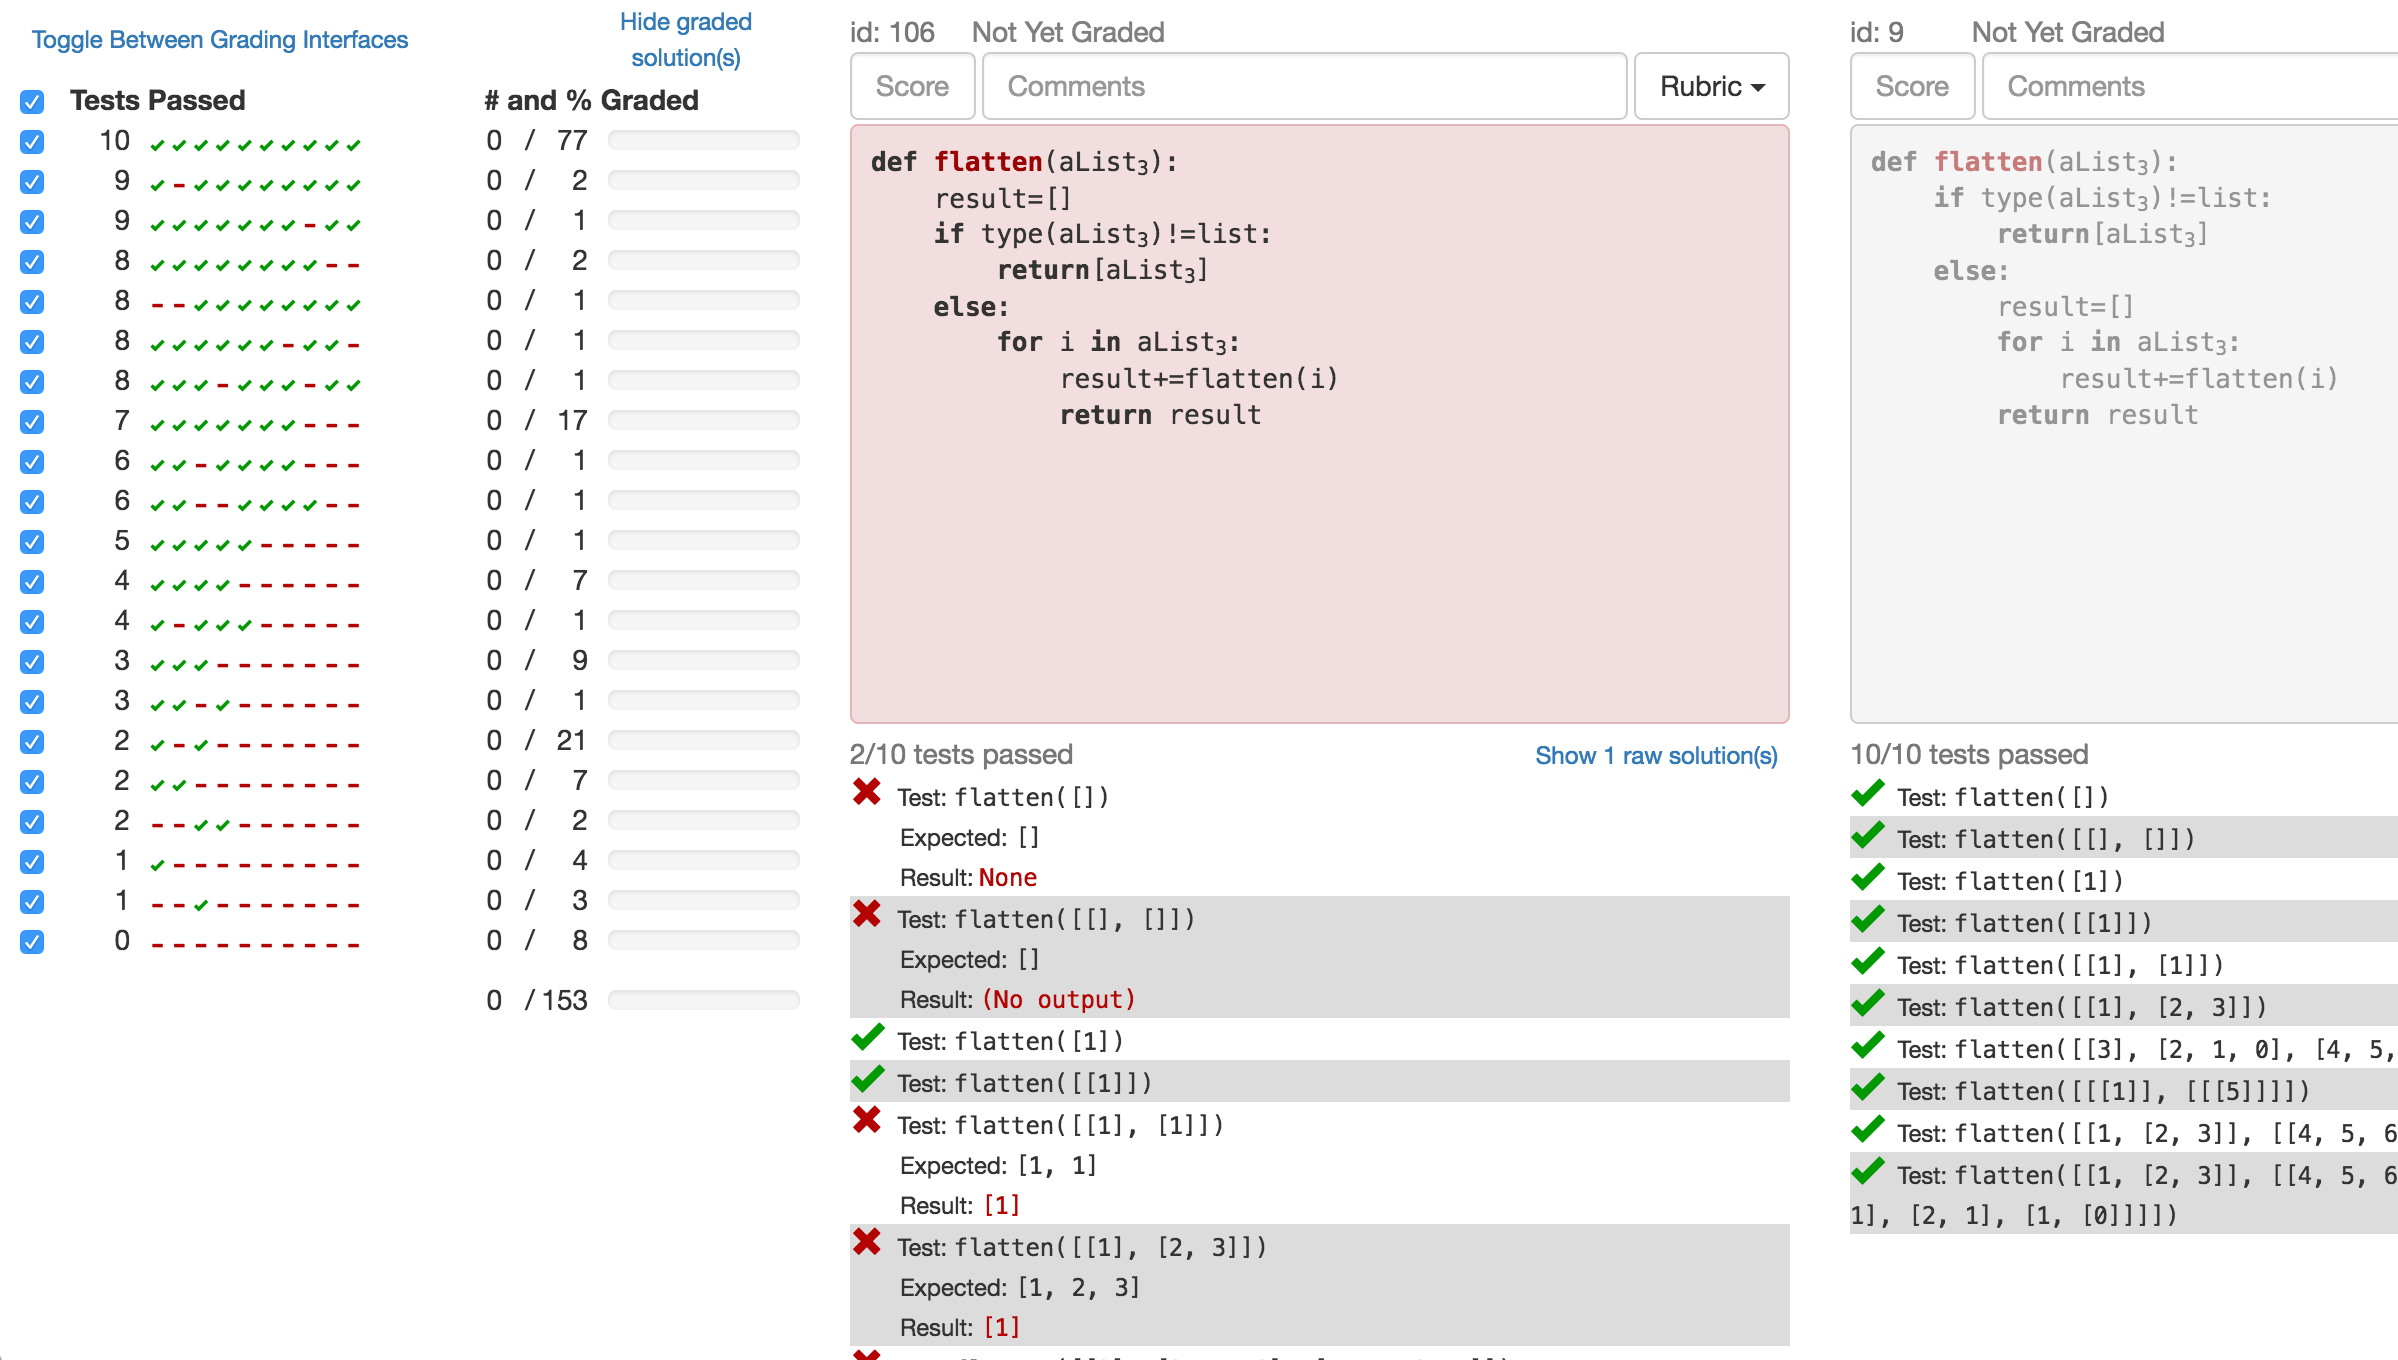
\includegraphics[width=\textwidth]{Body/figures/grovercode/figure_1}
\caption{The GroverCode user interface displaying solutions to an introductory Python programming exam problem, in which students are asked to implement a function to flatten a nested list of arbitrary depth.
}
\label{fig:whole_interface}
\end{figure} 

\begin{figure*}[t!]
    \centering
    \begin{subfigure}[b]{0.5\textwidth}
        \centering
        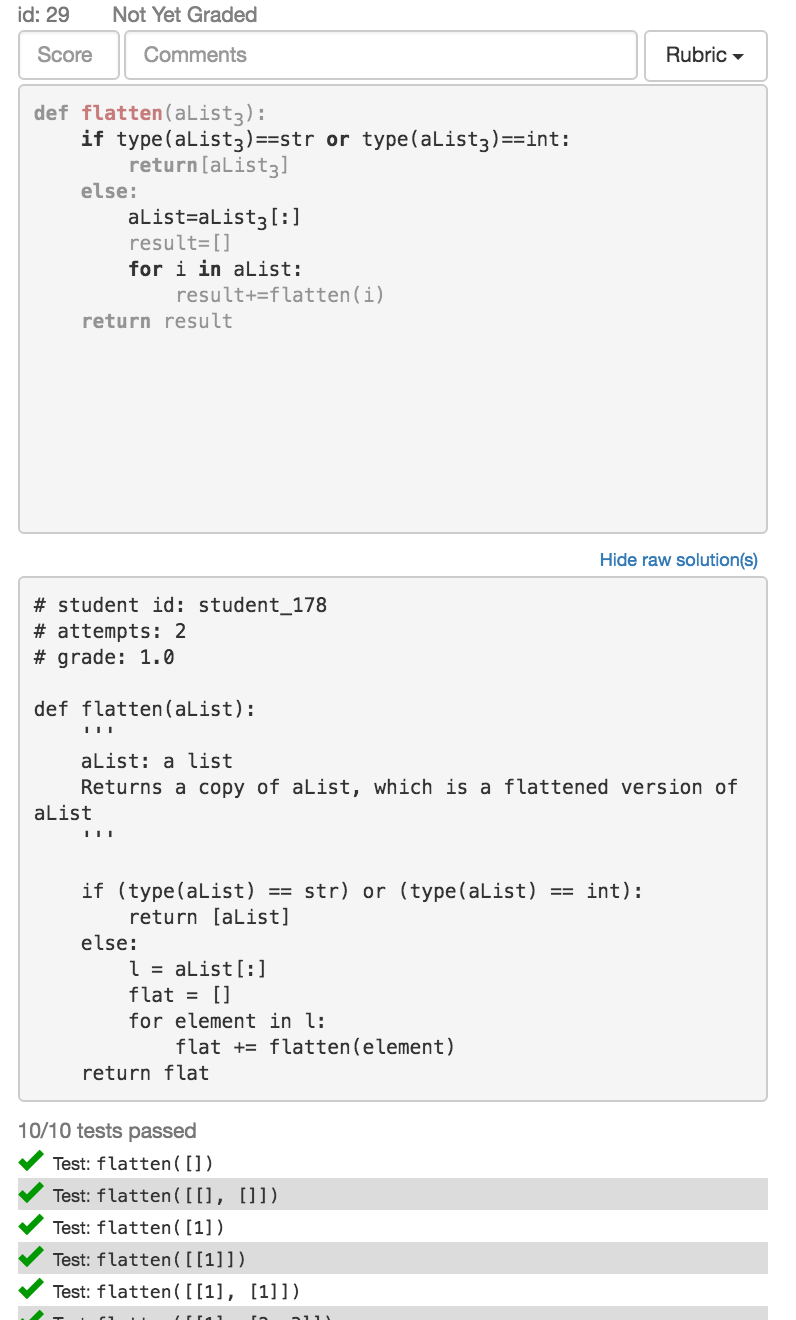
\includegraphics[height=4in]{Body/figures/grovercode/figure_2}
        \caption{A correct solution, its corresponding raw solution, and its performance on test cases, as displayed in GroverCode.}
        \label{fig:correct_stack}
    \end{subfigure}%
    ~ 
    \begin{subfigure}[b]{0.5\textwidth}
        \centering
        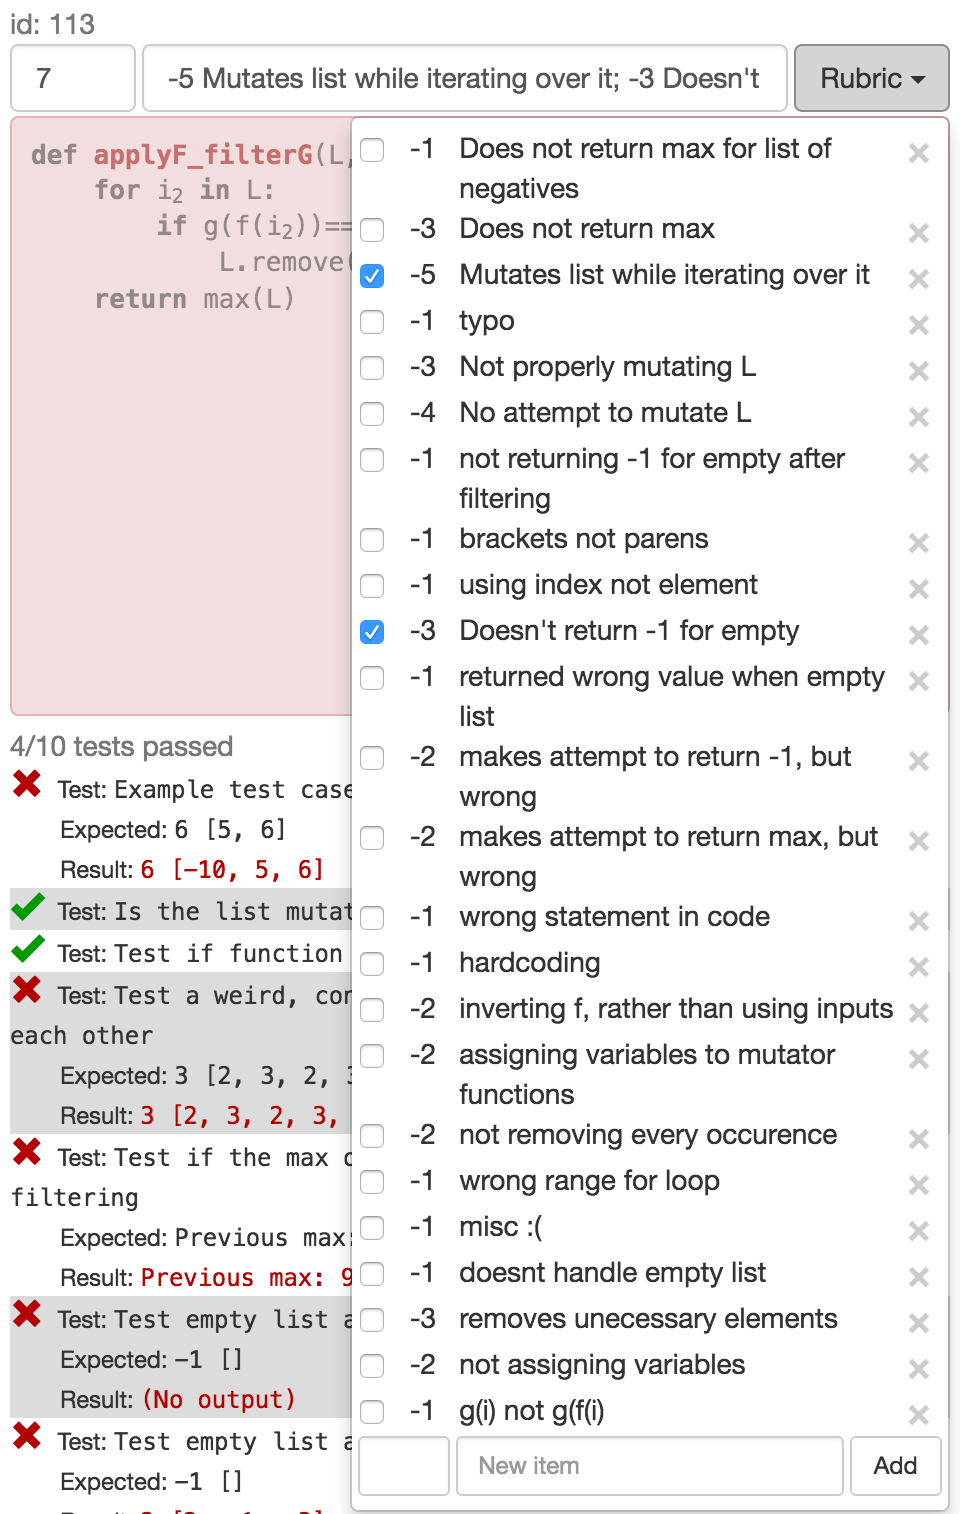
\includegraphics[height=4in]{Body/figures/grovercode/figure_3}
        \caption{An incorrect solution with the rubric dropdown menu open. Text for each of the checked items is automatically inserted in the comment box.}
        \label{fig:rubric}
    \end{subfigure}
    \caption{Correct and incorrect solutions, as rendered by GroverCode.}
\label{fig:correct_and_incorrect_stacks}
\end{figure*}

% \begin{figure}
% \centering
% 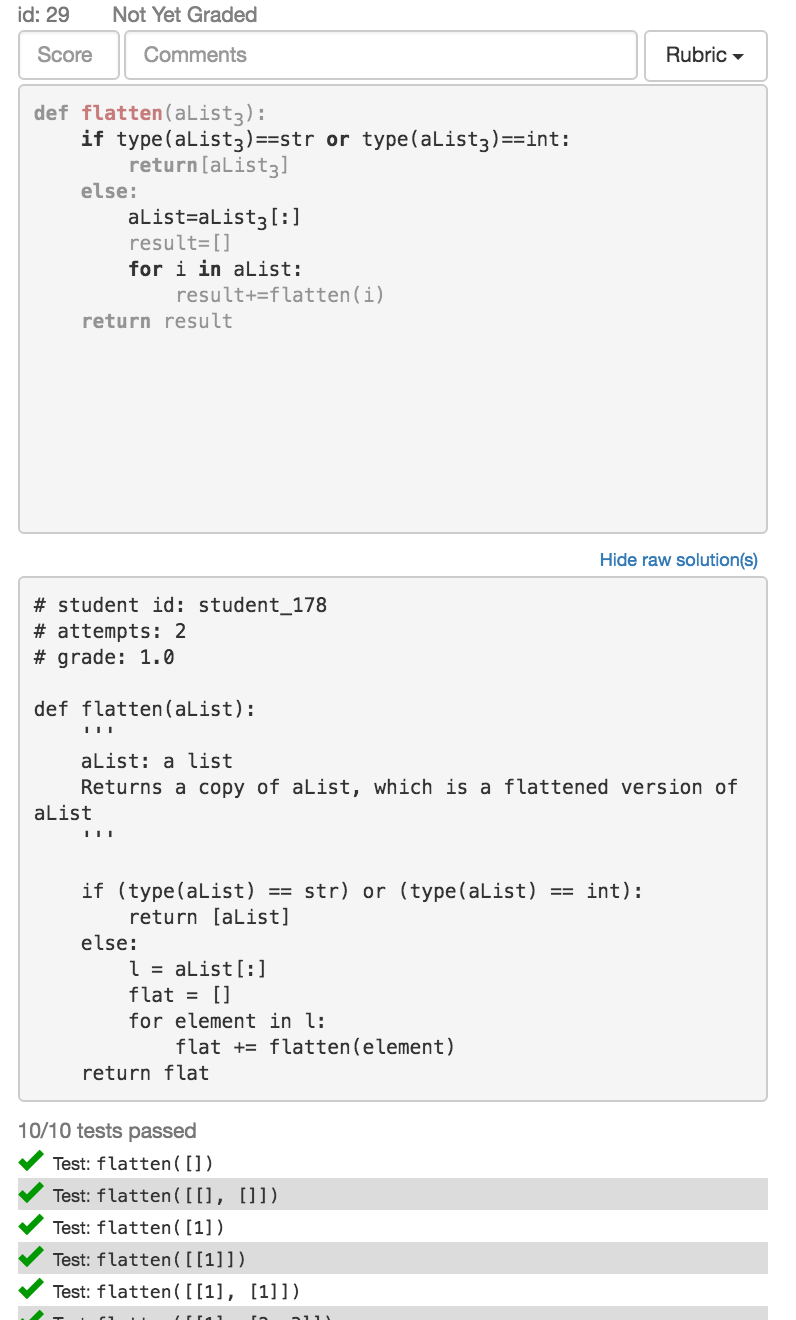
\includegraphics[width=0.5\textwidth]{Body/figures/grovercode/figure_2}
% \caption{A correct solution, its corresponding raw solution, and its performance on test cases, as displayed in GroverCode.}
% \label{fig:correct_stack}
% \end{figure}

% \begin{figure}
% \centering
% 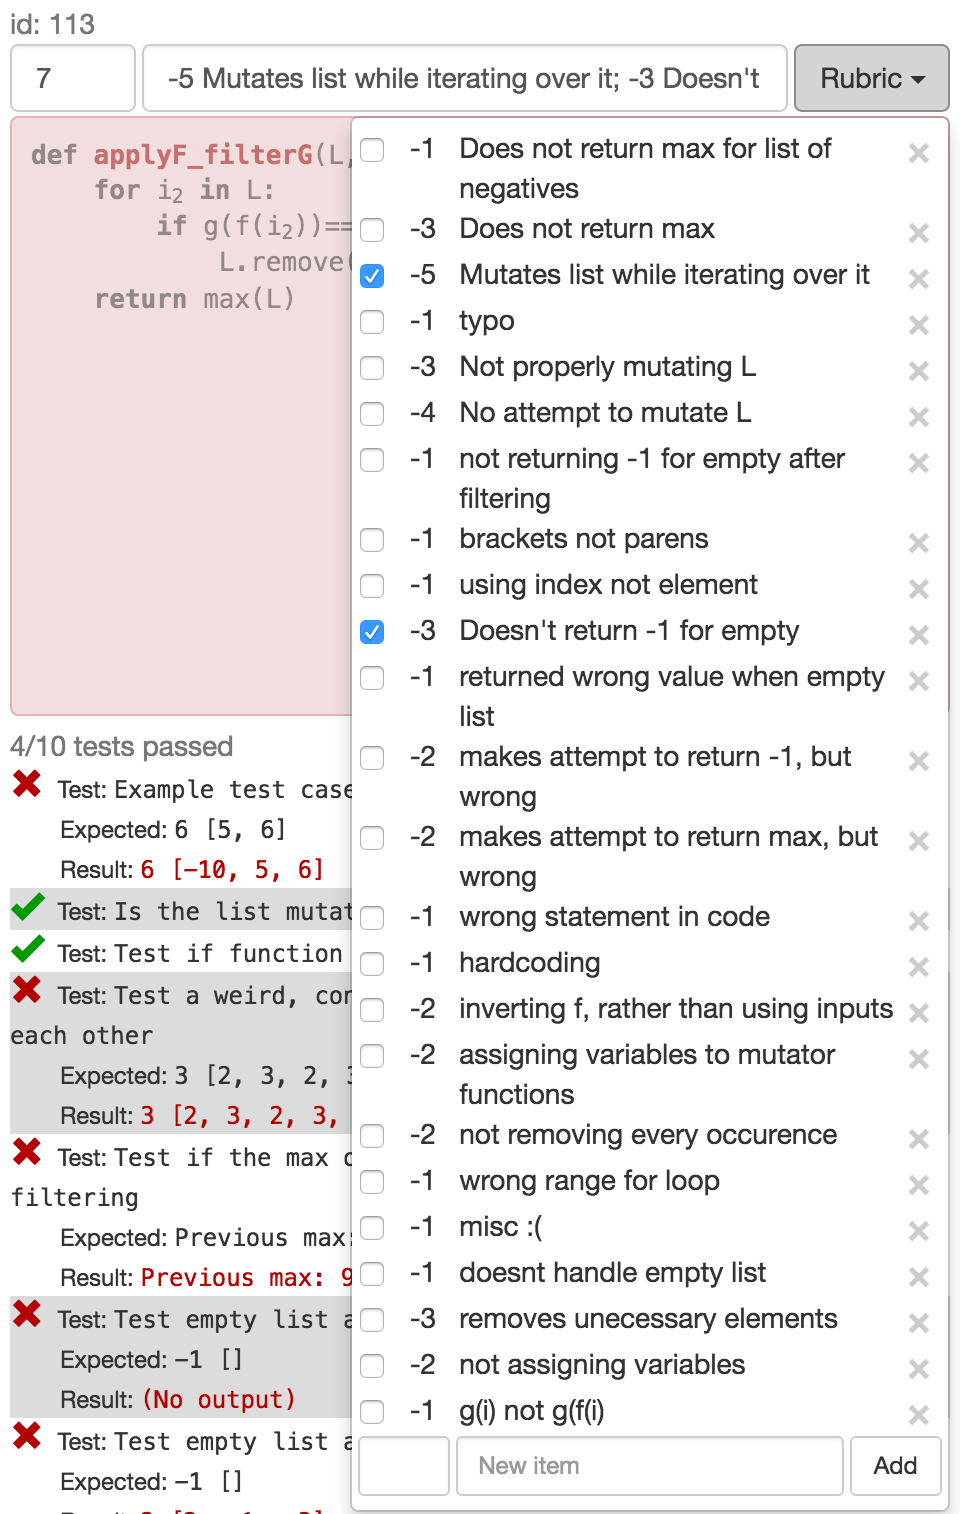
\includegraphics[width=0.5\textwidth]{Body/figures/grovercode/figure_3}
% \caption{A stack with the rubric dropdown menu open. Text for each of the checked items is automatically inserted in the comment box.}
% \label{fig:rubric}
% \end{figure}

The panel of progress indicators and filters, shown on the left side of Figure~\ref{fig:whole_interface}, helps teachers understand the distribution of solution behavior on test cases, track their grading progress, and grade sets of solutions that fail the same test cases one at a time. The rows of aligned sequences of green checks and red dashes represent error vectors, i.e., the pass/fail results with respect to the ordered list of teacher-specified test cases. The checkbox next to each error vector allows the teacher to selectively view subsets of solutions based on the particular tests they pass and fail. Solutions with the same error vectors may include similar mistakes. 

Like OverCode, GroverCode groups correct solutions into stacks. Grades are propagated to all the solutions in a stack. OverCode does not group incorrect solutions into stacks because the stacking process for incorrect solutions is too new and experimental for field deployment in an actual grading session. GroverCode still normalized all solutions, both correct and incorrect.

The grading performed by the 6.0001 staff was intellectually demanding. For example, many staff members attempted to correct incorrect solutions by hand to better undertstand how far off the student was from a correct answer. When raw solutions are shown in random order, one solution may have a different approach, behavior, and appearance from the next. The transition from grading one solution to the next can mean starting from scratch. In an attempt to minimize the cognitive load of switching from one solution to the next, the GroverCode user interface includes the following features:
\begin{itemize}
\item Horizontally aligned solutions for side-by-side comparison
\item Easy filtering of solutions by input-output behavior, i.e., their error vectors
\item Normalized variable names
\item Solutions ordered to minimize the distance between adjacent solutions with respect to a custom similarity metric defined in Stacey Terman's Master's of Engineering thesis~\cite{staceythesis}
\item Highlighted lines of code in each solution which differ from the previous solution in the horizontal list
\end{itemize}

In OverCode, a single-line difference between two solutions that affects variable behavior causes the variable renaming process to propagate naming differences to every line that mentions the affected variables. This non-locality of difference makes it harder to spot where the original syntactic difference between two platonic solutions is. As a result, the rendering of stacks in the GroverCode user interface is slightly different than in OverCode. Even if the normalized variable names are different between two syntactically identical lines of code in two different stacks, if the variables take on the same sequence of values {\it just within that line of code}, it will not be highlighted as different in the user interface. Only the line with the original syntactic difference will be highlighted.


\subsubsection{Implementation}~\label{subsec:grovercodepipeline}

The GroverCode implementation is a modification of the OverCode pipeline. Solutions which return an expected output for all test cases during the preprocessing step are categorized as correct, and all other solutions, having failed at least one test case, are categorized as incorrect. Correct solutions are normalized by the same process as was used in the original OverCode. 

In the original OverCode pipeline for correct solutions, variable behavior is assumed to hold enough semantic information to be the sole basis on which variable names are normalized. GroverCode applies this rule to incorrect solutions as well, but only for variables whose behavior matches a common variable in the correct solutions. This step may be error prone. Incorrect solutions are known to be wrong with respect to input-output behavior, the behavior of the variables within them is suspect too, even if it happens to match a common variable in a correct solution. %if a variable in an incorrect solution has the same behavior as a common variable in the correct solutions, GroverCode will rename the variable in the incorrect solution so it matches the common variable's name in the correct solutions.

%However, this renaming strategy may change in future versions of GroverCode because, 

In incorrect solutions, syntax, e.g., the operations applied to a variable, may be more helpful for normalizing variable names than behavior. For example, in an incorrect solution, a variable $i$ may be operated or depended on exactly the same way as a common variable in a correct solution. However, if an error somewhere else in the solution causes $i$ to behave differently, the original method of identifying common variables will be thrown off. %Based on this example, variables in incorrect solutions that are not already renamed based on behavior are renamed based on syntax.

The OverCode pipeline is modified for GroverCode to capture this syntactic information. The modified pipeline examines the program trace collected during preprocessing and the AST for each solution and compiles the following information for each line of code in each solution:
\begin{enumerate}
\item a template, i.e., the line of code with variables replaced by blanks, e.g., \texttt{\underline{\hspace{1em}} += 1} and \texttt{for \underline{\hspace{1em}} in range(\underline{\hspace{1em}}):}
\item an ordered list of the common variable behaviors and their normalized names corresponding to each blank in the line, e.g., the blank in \texttt{\underline{\hspace{1em}} += 1} can be associated with one of several common variables, depending on the rest of the solution
\item an ordered list of the sequences of values each blanked-out variable in the line took on during execution, e.g., the first blank in \texttt{for \underline{\hspace{1em}} in range(\underline{\hspace{1em}}):} might iterate through \texttt{1,2,3} while, with each visitation of this line during execution, the second blank stays constant at \texttt{[1,2,3],[1,2,3],[1,2,3]}
\end{enumerate}
Item 1 in this list, the template, captures the syntax of the line, ignoring the variables mentioned in it. Items 1 and 2 in this list together capture the information necessary to reconstruct the original normalized lines in OverCode. Items 1 and 3 capture the information necessary to tell what the variable behavior is just within that one line and whether two lines in two different stacks will be highlighted as different from each other. This information is also used for variable renaming in incorrect solutions.

\begin{table}
\centering
%Copied with permission from Terman~\cite{staceythesis}}\todo{get explicit permission}
\begin{tabular}{l l r}
%\hline
 &  & {\bf Location} \\
{\bf Example line of code} & {\bf Template} & {\bf of \texttt{exp}} \\
\hline
\footnotesize{\texttt{def power(base, exp):}} & \footnotesize{\texttt{def power(\underline{\hspace{1em}}},\underline{\hspace{1em}}):} & 1 \\
%\hline
\footnotesize{\texttt{while index <= exp:}} & \footnotesize{\texttt{while \underline{\hspace{1em}}<=\underline{\hspace{1em}}:}} & 1 \\
%\hline
\footnotesize{\texttt{return 1.0*base*power(base, exp-1)}} & \footnotesize{\texttt{return 1.0*\underline{\hspace{1em}}*\underline{\hspace{1em}}*power(\underline{\hspace{1em}},\underline{\hspace{1em}}-1)}} & 3 \\
%\hline
\footnotesize{\texttt{return base*power(base, exp-1)}} & \footnotesize{\texttt{return \underline{\hspace{1em}}*power(\underline{\hspace{1em}},\underline{\hspace{1em}}-1)}} & 2 \\
%\hline
\footnotesize{\texttt{return power(base, exp-1)*base}} & \footnotesize{\texttt{return power(\underline{\hspace{1em}},\underline{\hspace{1em}}-1)*\underline{\hspace{1em}}}} & 1 \\
%\hline
\footnotesize{\texttt{ans = base*power(base, exp-1)}} & \footnotesize{\texttt{\underline{\hspace{1em}}=\underline{\hspace{1em}}*power(\underline{\hspace{1em}},\underline{\hspace{1em}}-1)}} & 3 \\
%\hline
\footnotesize{\texttt{if exp <= 0:}} & \footnotesize{\texttt{if \underline{\hspace{1em}}<=0:}} & 0 \\
%\hline
\footnotesize{\texttt{if exp == 0:}} & \footnotesize{\texttt{if \underline{\hspace{1em}}==0:}} & 0 \\
%\hline
\footnotesize{\texttt{if exp >= 1:}} & \footnotesize{\texttt{if \underline{\hspace{1em}} >= 1:}} & 0 \\
%\hline
\footnotesize{\texttt{assert type(exp) is int and exp >= 0}} & \footnotesize{\texttt{assert type(\underline{\hspace{1em}}) is int and \underline{\hspace{1em}}>=0}} & 0, 1 \\
%\hline
\end{tabular}
\caption{\textbf{Example:} All templates and locations in which the abstract variable \texttt{exp}, the second argument to a recursive \texttt{power} function, appears. A location represents the index or indices of the blanks that the abstract variable occupies, where the first blank is index 0, the second is index 1, and so on. The second and third columns together form a template-location pair.} 
\label{tab:templatelocation}
\end{table}

The GroverCode normalization process uses this syntactic information, in addition to behavior, to identify and rename common variables. The template of a line, e.g., \texttt{for \underline{\hspace{1em}} in \underline{\hspace{1em}}:} is the syntax of the line with variable names removed. For each common variable in correct solutions, GroverCode counts how many times it appears in each template and in which location, represented as an index into the blanks in the template. Examples of templates and locations are shown in \autoref{tab:templatelocation}. If a yet-unrenamed variable in an incorrect solution appears in the exact same template-locations as a common variable in a correct solution, it will be renamed to match that common variable. If a variable in an incorrect solution is still not normalized, the counts of template-locations associated with each common variable in the correct solutions are used, as described in detail in Terman~\cite{staceythesis}, to infer the most likely common variable it could be renamed to, as long as a threshold for similarity is met. Otherwise, its original name is kept.





\subsubsection{Field Deployment}

Approximately two hundred students enrolled in 6.0001 during the spring 2016 semester, and nine instructors used GroverCode to grade nearly all student solutions. %Seven programming problems of a variety of difficulties were graded over the course of these two sessions.
The GroverCode analysis pipeline was run on both the midterm and final exam problems from the Spring 2016 semester of 6.0001, which had approximately 200 students enrolled. These exams contained seven programming problems in total, and between 133 and 189 solutions per problem made it through the analysis pipeline to be displayed in the user interface. The midterm problem prompts were:
\begin{itemize}
\item \texttt{power} (q4): Write a recursive function to calculate the exponential \texttt{base} to the power \texttt{exp}.
\item \texttt{give\_and\_take} (q5): Given a dictionary \texttt{d} and a list \texttt{L}, return a new dictionary that contains the keys of \texttt{d}. Map each key to its value in \texttt{d} plus one if the key is contained in \texttt{L}, and its value in d minus one if the key is not contained in \texttt{L}.
\item \texttt{closest\_power} (q6): Given an integer base and a target integer \texttt{num}, find the integer exponent that minimizes the difference between \texttt{num} and \texttt{base} to the power of exponent, choosing the smaller exponent in the case of a tie.
\end{itemize}
The final problem prompts were:
\begin{itemize}
\item \texttt{deep\_reverse} (q4): Write a function that takes a list of lists of integers \texttt{L}, and reverses \texttt{L} and each element of \texttt{L} in place.
\item \texttt{applyF\_filterG} (q5): Write a function that takes three arguments: a list of integers \texttt{L}, a function \texttt{f} that takes an integer and returns an integer, and a function \texttt{g} that takes an integer and returns a boolean. Remove elements from \texttt{L} such that for each remaining element \texttt{i}, \texttt{f(g(i))} returns \texttt{True}. Return the largest element of the mutated list, or -1 if the list is empty after mutation.
\item \texttt{MITCampus} (q6): Given the definitions of two classes: \texttt{Location}, which represents a two-dimensional coordinate point, and \texttt{Campus}, which represents a college campus centered at a particular \texttt{Location}, fill in several methods in the \texttt{MITCampus} class, a subclass of \texttt{Campus} that represents a college campus with tents at various \texttt{Locations}.
\item \texttt{longest\_run} (q7): Write a function that takes a list of integers \texttt{L}, finds the longest run of either monotonically increasing or monotonically decreasing integers in \texttt{L}, and returns the sum of this run.
\end{itemize}
For each problem processed during the field deployments, an example of a staff-written correct solution is included in the Appendix.

Using the GroverCode user interface, nine instructors, including one lecturer and eight teaching assistants (TAs) graded these solutions as part of their official grading responsibilities. Stacey Terman, the Master's of Engineering student who implemented most of GroverCode, was one of these TAs. GroverCode logged TA grading events, such as adding or applying rubric items and point values to solutions. TAs hand-graded solutions that did not successfully pass through the GroverCode pipeline. The observer (the author of this thesis) took extensive notes during each day-long grading session to capture spontaneous feature requests as well as bugs and complaints. 

%\begin{comment}
% {\bf Programming Exam Problems}

%Given the increasing difficulty of these exam problems, the following numbers dropped between the midterm and the final: the number of students present to take the exam, the number of students who submitted any solution to a given problem before the test period ended, and the number of correct solutions that could be clustered.

\subsubsection{Pipeline Evaluation}

Table~\ref{table:num_submissions} shows the number of solutions submitted for each problem and the number successfully processed by the GroverCode pipeline. Table~\ref{table:cluster_stats} captures the scale of the variation as well as some clustering statistics. Table~\ref{table:renametype} summarizes the counts of the various mechanims by which variables in incorrect solutions were normalized.

\begin{table}[h!]
\centering
\begin{tabular}{l r|r|r|r|r|r|r}
%\hline
& \multicolumn{3}{c}{Quiz} & \multicolumn{4}{c}{Final} \\
%\cline{2-8}
& q4 & q5 & q6 & q4 & q5 & q6 & q7 \\
\hline
Submissions & 193 & 193 & 193 & 175 & 173 & 170 & 165 \\
\hline
Mean lines per solution & 9.9 & 16.9 & 19.8 & 12.3 & 20.9 & 50.0 & 41.8 \\
\hline
Solutions & 186 & 189 & 168  & 170 & 166  & 134 & 133 \\
successfully processed & 96\% & 98\% & 87\% & 97\% & 96\% & 79\% & 81\% \\
%\hline
\end{tabular}
\caption{Number of solutions submitted and successfully processed by GroverCode for each problem in the dataset. Reasons why a solution might not make it through the pipeline include syntax errors and memory management issues caused by students making inappropriate function calls.}
\label{table:num_submissions}
\end{table}

\begin{table}[!ht]
\centering
\begin{tabular}{l r|r|r|r|r|r|r}
%\hline
& \multicolumn{3}{c}{Quiz} & \multicolumn{4}{c}{Final} \\
%\cline{2-8}
& q4 & q5 & q6 & q4 & q5 & q6 & q7 \\
\hline
Correct solutions & 182 & 160 & 94 & 96 & 49 & 16 & 12 \\
 & 94\% & 82\% & 49\% & 55\% & 28\% & 9\% & 7\% \\
\hline
Incorrect solutions & 4 & 29 & 74 & 74 & 117 & 118 & 121 \\
\hline
Test cases & 10 & 15 & 25 & 11 & 10 & 17 & 28 \\
\hline
Distinct error signatures & 6 & 16 & 36 & 12 & 38 & 57 & 42 \\
\hline
Correct stacks & 40 & 84 & 93 & 47 & 46 & 16 & 12 \\
\hline
Stacks with > 1 solution & 13 & 18 & 1 & 8 & 2 & 0 & 0 \\
\hline
Solutions in stacks & 151 & 94 & 2 & 57 & 5 & 0 & 0 \\
%\hline
\end{tabular}
\caption{The degree of variation in input-output behavior and statistics about stack sizes.}
\label{table:cluster_stats}
\end{table}

\begin{table}
\centering
\begin{tabular}{l c|c|c|c|c|c|c}
%\hline
& \multicolumn{3}{c}{Quiz} & \multicolumn{4}{c}{Final} \\
%\cline{2-8}
& q4 & q5 & q6 & q4 & q5 & q6 & q7 \\
\hline
Variables in incorrect submissions & 15 & 149 & 482 & 289 & 550 & 559 & 859 \\
\hline
Variables renamed based on values & 14 & 84 & 266 & 97 & 246 & 97 & 187 \\
\hline
Variables renamed based on templates & 0 & 58 & 166 & 136 & 264 & 188 & 489 \\
\hline
Variables not renamed & 1 & 7 & 50 & 56 & 40 & 274 & 183 \\
%\hline
\end{tabular}
\caption{Statistics about variables renaming based on different heuristics in the GroverCode normalization process.}
\label{table:renametype}
\end{table}
%\end{comment}
 
\subsubsection{Discussion}

GroverCode was particularly appreciated on simpler problems where GroverCode clustered correct solutions together to be graded by a single action. Under these conditions, the clustering capability GroverCode inherits from OverCode amplified teacher effort.

Variable renaming was, for simpler programming problems, an invisible and possibly slightly confusing helping hand. One grader remarked, out loud: ``Why is everyone naming their iterator variable `i'?'' at which point he had to be reminded of the variable renaming process. 

When applied to more complex solutions, the normalization process was at times more harmful than helpful for teacher comprehension. As solutions became more varied and structurally complex, graders started toggling off normalization because the renaming of variables, removal of comments, and formatting standardization was removing clues they needed in order to understand student intent.

The feature for grouping solutions based on their behavior on test cases was appreciated regardless of solution complexity. While it was difficult to get direct feedback on the helpfulness of pair-wise difference highlighting and optimized solution ordering, graders heavily used and appreciated the ability to filter and grade solutions one error vector at a time. At least one grader remarked aloud that it seemed like many of the solution with the same error vector made similar mistakes. Therefore filtering by error vector may have been one of the stronger contributors to any hypothetical decreased cognitive load due to using GroverCode over the status quo of random assignment to solutions in a CSV file.

%\todo{DNHT: add to related work Appropriately chosen latent variable models have already been used in the past to model open-source code and answers to open-response mathematical questions.}

\section{Conclusion}
OverCode is a novel system for visualizing thousands of Python programming solutions that helps teachers explore the variations among them. Unlike previous approaches, OverCode uses a lightweight static and dynamic analysis to generate platonic solutions that represent stacks of similar solutions in an interactive user interface. It allows teachers to filter stacks by normalized lines of code and to further merge different stacks by composing rewrite rules. As observed in two user studies with a total of 24 current and potential teaching assistants, OverCode allowed teachers to more quickly develop a high-level view of students' understanding and misconceptions, and provide feedback that is relevant to more student solutions. 

GroverCode, an extension of OverCode which handles incorrect solutions, is a new tool for triaging and hand-grading solutions. It was successfully deployed in the field as the tool for grading the midterm and final exams of MIT's 6.0001 course, ``Introduction to Computer Science and Programming in Python''. Based on teachers' appreciation of the interface over the existing alternatives, GroverCode will continue to be deployed in the field to ease the subjective psychological burden of grading hundreds of Python programs. %I believe an information visualization approach is necessary for teachers to explore the variations among solutions at the scale of MOOCs, and OverCode is an important step towards that goal.
%\todo{make sure evidence of teacher's appreciate is included}
\chapter{Design of antimicrobial peptides}\label{chapter:amps}
\begin{comment}
\section{Introduction}
    In the previous chapter, I introduced grammars as a generalized
    method for modeling motifs in sequences of characters.  In
    addition, I presented a detailed look at the Teiresias motif
    discovery tool.  In this, the second chapter of my thesis, I
    show how Teiresias can be used to derive sets of regular
    grammars describing a particular class of protein sequences ---
    antimicrobial peptides.  In what follows, I present a general
    background on antimicrobial peptides and then provide a
    rationale for why these peptides are particularly well--suited
    for being modeled using regular grammars.  I detail the
    construction of an annotation tool for finding new antimicrobial
    peptides and validating the general hypothesis that regular
    grammars can be used as a sensitive and specific indicator of
    antimicrobial function in peptide sequences.  Next, I describe
    the preliminary design of synthetic antimicrobial peptides using
    an evolutionary approach, which, although ultimately inconclusive, provided
    motivation for a more focused design.  The final section of this
    chapter describes a more focused design approach, detailing the
    successful construction of numerous novel peptides with strong
    antimicrobial activity against a wide spectrum of bacteria.

    The research described in this chapter is drawn
    largely from a publication that is in preparation
    in collaboration with Christopher Loose, Isidore
    Rigoutsos, and Gregory Stephanopoulos.  (Some
    experimental work in Section~\vref{section:preliminary}
    was also performed by Gyoo Yeol Jung.)  Throughout this
    chapter, the use of the pronoun ``we'' refers to this
    group of authors.

\section{Motivation}
    Antimicrobial peptides are small
    proteins that attack and kill microbes.
    These peptides are effectors of the
    innate immune system: the phylogenetically
    ancient first line of defense against pathogen
    assault~\cite{rolff2003invertebrate,kimbrell2001evolution}.
    Antimicrobial peptides are ubiquitous
    amongst multicellular eukaryotes and
    found in diverse contexts including frog
    skin~\cite{simmaco1999antimicrobial}, scorpion
    venom~\cite{moerman2002antibacterial}, and human
    sweat~\cite{schittek2001dermcidin}.

    There is a growing interest in antimicrobial
    peptides, due largely to the proliferation
    of multi--drug resistant pathogen
    strains~\cite{cassell2001development}.  These
    strains are resistant to one or more common
    antibiotics such as penicillin, tetracylin,
    or vanocomycin.  In the United States alone,
    the cost of treating and preventing infections by
    these pathogens is estimated to be many billions of
    dollars annually~\cite{harrison1998antimicrobial}.
    In the arms race against microbes,
    mankind is losing --- only a single new
    class of antibiotics was developed in the
    past 30 years~\cite{normark2002evolution,
    walsh2000molecular}.  However, there is mounting
    evidence that antimicrobial peptides are less
    likely to induce bacterial resistance and will make
    a strong contribution to our therapeutic arsenal
    ~\cite{zasloff2002antimicrobial,zasloff2002antimicrobialpeptides,ge1999invitro}.

    Human antimicrobial peptides, such as
    the defensins and cathelicidins, help to
    maintain a passive defense against pathogens
    in the environment.  A malfunction of these
    peptides leads to severely immunocompromised
    phenotypes.  For example, a deficiency of the
    LL-37 cathelicidin leads to morbus Kostmann,
    a congenital neutropenia characterized
    by recurrent bacterial infection and short
    life--expectancy~\cite{putsep2002deficiency,bowman2003antibacterial}.
    In addition, the pathogenesis of cystic fibrosis
    (CF) is indirectly caused by antimicrobial peptide
    impairment~\cite{ganz2003defensins}.  CF patients
    have a defective Cl$^-$ ion channel in the
    pulmonary airway epithelia that causes unusually
    high salt concentrations.  The salt disrupts the
    function of the epithelial defensins, leading
    to chronic infections and ensuing respiratory
    failure~\cite{smith1996cystic,zasloff2002antimicrobial}.
    More severe phenotypes have been produced in
    loss--of--function animal models.  For example,
    Wilson \emph{et. al.}~\cite{wilson1999regulation}
    showed that mice with depressed defensin
    activity required a 10--fold lower dose
    of the \emph{S. typhimurium} pathogen
    to produce a fatality.  In contrast,
    gain--of--function mice expressing human
    enteric defensin HBD--5 have a markedly
    increased resistance to \emph{S. typhimurium}
    assault~\cite{salzman2003protection}.

    In addition to their more publicized
    antibiotic capabilities, antimicrobial peptides
    appear to be important in a variety of other
    diseases.  For example, the antimicrobial
    peptides of \emph{Anopheles gambiae},
    the malaria mosquito, are upregulated
    after malaria (\emph{Plasmodium berghei})
    infection~\cite{christophides2002immunity}
    and, in some cases, are capable
    of killing the ookinetes of the
    parasite~\cite{barillas2000mosquito,vizioli2001gambicin}.
    Antimicrobial peptides are also indicated in a
    resistance to the AIDS--causing virus, HIV\@.
    Long--term HIV nonprogressors display
    elevated levels of $\alpha$--defensins
    that inhibit the proliferation of the
    virus~\cite{zhang2002contribution}.
    Finally, a limited class of antimicrobial
    peptides may form the basis for novel cancer
    treatments~\cite{kim2003invitro,ellerby1999anticancer}.
    For example, the antimicrobial peptide
    tachyplesin can repress the growth of cancerous
    tumors both \emph{in vitro} and \emph{in
    vivo}~\cite{chen2001rgdtachyplesin}.

    The many disease--relevant behaviors of
    antimicrobial peptides are a result of their
    ability to broadly distinguish eukaryotic
    cells from pathogenic invaders.  There are two
    features that give the peptides this ability:
    a net positive charge and an amphipathic 3--D
    structure~\cite{giangaspero2001amphipathic,epand1999diversity}.
    These features endow the peptide with an
    affinity for negatively charged outer leaflet
    of the bacterial cytoplasmic membrane (see
    Figure~\vref{fig:peptideAction}).  This affinity
    leads to permeablization of the bacterial membrane,
    which is the basis for the bactericidal activity
    of antimicrobial peptides.  Although this mode
    of action is common to almost all antimicrobial
    peptides, there are many diverse primary sequences
    that can produce this behavior.  These sequences
    form a handful of conserved families, the most
    common of which are the $\alpha$--helical
    and $\beta$--sheet antimicrobial peptides
    ~\cite{tossi2000amphipathic}.

    \begin{figure}[phtb] \centering
    \includegraphics[width=0.70\textwidth]{Body/Images-chap2/attack2.png}
    \caption[Antimicrobial peptide action]{
        Antimicrobial peptide action.  In the
        figure above, amphipathic antimicrobial
        peptides with net positive charges are
        attracted via electrostatic forces to
        the negatively charged outer--leaflet
        of the microbial membrane (step
        1)~\cite{zasloff2002antimicrobial}.  This
        membrane is either the lipopolysaccharide
        layer or the peptidoglycan layer of
        gram--negative and gram--positive bacteria,
        respectively~\cite{epand1999diversity}.
        In addition, the $\beta$--1,3--glucan in
        fungal membranes and the phosphoglycan
        of certain parasites can give membrane
        characteristics that are exploited
        by certain classes of antimicrobial
        peptides.  The peptides cover and lyse
        the membrane via either a ``barrel
        stave'' or ``carpet'' mechanism (step
        2)~\cite{shai2002mode}.  Although some
        antimicrobial peptides are hemolytic,
        in general, they are not damaging to
        multicellular organisms because 1) the
        negatively charged phosphatydilserines
        of their outer leaflet are sequestered
        on the cytoplasmic side of the membrane,
        and 2) the membranes are stabilized by
        cholesterols~\cite{zasloff2002antimicrobial}.
    } \label{fig:peptideAction} \end{figure}


Figure~\vref{fig:aurein} shows the structure of aurein--1.2, an
archetypal alpha helical antimicrobial peptide from the Australian
Southern bell frog~\cite{wang2005correlation}.  Alpha helical AmPs
form the largest single family of AmPs.  They are particularly
common in amphibians because species such as frogs tend to inhabit
wet and warm ecological niches that are conducive to the
proliferation of bacteria.  (See Figure~\ref{fig:frogAmps} for a
phylogenetic tree of the more than 400 amphibian AmPs.)  Alpha
helical AmPs tend, in general, to have a amphipathic structure in
which positively charged residues are segregated on to a particular
side of the longitudinal axis of the helix.  Negatively charged or
neutral residues tend to be isolated on the opposite side from the
positively charged residues.  Evidence suggests that this
confirmation allows the peptide to position itself judiciously
relative to the bacterial membrane, facilitating entry of the
peptide into the membrane and, ultimately, membrane
disruption~\cite{zasloff2002antimicrobial}.

        \begin{figure}[ptb]
        A) Ball and stick
        \begin{center}
        \includegraphics[width=2.0in]{Body/Images-chap2/1vm5-balls.png}
        \end{center}

        \smallskip
        B) Ribbon
        \begin{center}
        \includegraphics[width=2.0in]{Body/Images-chap2/1vm5-ribbon.png}
        \end{center}

        \smallskip
        C) Peptide wheel view
        \begin{center}
        \includegraphics[angle=90,width=2.0in]{Body/Images-chap2/pepwheel.pdf}
        \end{center}
        \caption[The structure of aurein]{The structure of aurein--1.2~\cite{wang2005correlation}.
            Aureins constitute a large family of secreted proteins
            originally isolated from the skin of frogs.
            This particular structure was isolated from the
            Australian Southern bell frog.  The peptide conforms to
            the classic amphipathic alpha helical structure and has wide--spectrum antimicrobial activity.
            Part A) shows a ball--and--stick representation of the
            structure in which nitrogen atoms are colored blue and
            oxygen atoms are colored red.  Part B) shows the same
            structure using a cartoon representation that clearly
            shows the alpha helix.  Finally, part C) shows a helical
            wheel projection in which uncharged residues are boxed
            in order to highlight the segregation of charges on the
            helix.  Graphics created using PyMol (DeLano Scientific,
        San Carlos, CA, USA).
        }
        \label{fig:aurein}
        \end{figure}

        \begin{sidewaysfigure}[ptb]
        \begin{center}
        \includegraphics[angle=270,width=0.9\textwidth]{Body/Images-chap2/frog-amps.pdf}
        \end{center}
        \caption[A phylogenetic tree of amphibian antimicrobial peptides]{
            A phylogenetic tree of amphibian AmPs.  Because they
            tend to inhabit environments that are conducive to the
            growth of bacteria, amphibians are under evolutionary
            pressure to develop numerous and varied AmPs.  This tree
            shows the degree of sequence similarity for over 400
            AmPs isolated from amphibian sources.  As the figure
            shows, amphibians have many families of AmPs, some of
            which are only distantly related, including the aureins,
            bombinins, bombesins, and brevinins.
        }
        \label{fig:frogAmps}
        \end{sidewaysfigure}

    The characteristic membrane--attack of
    antimicrobial peptides is the primary
    rationalization of the peptides' propensity to
    not induce bacterial resistance to the same
    degree as small molecule pharmaceuticals.
    That is, because the peptides leverage a
    pervasive polygenic trait of bacteria, the
    structure of the cell wall, it is ``expensive''
    for the bacteria to evolve a resistance
    ~\cite{zasloff2002antimicrobial,zasloff2002antimicrobialpeptides}.
    For this reason, many companies are developing
    therapeutics based on antimicrobial
    peptides, many of which are in phase III
    FDA trials ~\cite{hancock2002clinical}.
    Even more encouraging, some peptides show
    strong \emph{in vitro} bactericidal activity
    against pathogen strains that have developed
    a resistance to multiple conventional
    antibiotics~\cite{ge1999invitro,tiozzo1998wide,strom2003pharmacophore}.

\section{A grammatical approach to annotating
AmPs}\label{section:annotation}
    Our preliminary studies of natural AmPs indicated that their
    amphipathic structure gives rise to a modularity among the different
    AmP amino acid sequences.  The repeated usage of sequence modules ---
    which may be a relic of evolutionary divergence and radiation ---
    is reminiscent of phrases in a natural language, such as English.
    For example, the grammar \texttt{Q.EAG.L.K..K} (the ``\texttt{.}'' is
    a ``wildcard'', which indicates that any amino acid will suffice at
    that position in the grammar) is present in over 90\% of cecropins,
    an AmP common in insects.  Based on this observation we modeled
    the AmP sequences as a formal language --- a set of sentences using
    characters from a fixed alphabet, in this case the alphabet of amino
    acid one--letter symbols~\cite{jurafsky2000speech}.

    We conjectured that the ``language of AmPs'' could be described
    by a set of regular grammars and that these grammars, in turn, could be used
    to annotate and design novel AmPs.  As discussed in
    Chapter~\ref{chapter:intro},
    regular grammars are, in
    essence, simple rules for describing the allowed arrangements of
    characters.  These grammars, such as the cecropin grammar mentioned
    previously, are commonly written as regular expressions and are
    widely used to describe patterns in nucleotide and amino acid
    sequences~\cite{searls2002language,hofmann1999prosite}.

    To find a set of grammars describing AmPs we used the
    Teiresias pattern discovery tool~\cite{rigoutsos1998combinatorial}
    (see Section~\vref{section:teiresias} to discover an
    exhaustive, maximal set of regular grammars in a collection of
    antimicrobial peptides assembled from a variety of sources.

    \subsection{Collecting a database of antimicrobial peptides}

    Our collection of known antimicrobial peptides was taken principally
    from two databases:
    the Antimicrobial Sequences
    Database (\amsdb) ~\cite{tossi2002antimicrobial} and
    \sptr ~\cite{bairoch2000swiss-prot}.
        The \amsdb~ contains
        about 750 antimicrobial peptides, all of which are
        a subset of \sptr .  Some of the entries in
        the \amsdb~ are sequence fragments that are derived
        from larger precursors via post--translational modification.
        We discarded these peptides unless the reported
        antimicrobial fragment comprised at least 80\% of the
        length of its parent sequence.  From the remaining
        entries, we selected all that were from eukaryotic organisms,
        including the complete length of the parent
        peptides in our database.



        \include{Body/Images-chap2/antimicrobialnames}

        \sptr~ is a database of about 120 thousand heavily annotated
        sequences.  Included in the  annotations are keywords grouping
        proteins into functional categories.  For our initial database
        of antimicrobial peptides we extracted all the eukaryotic
        sequences matching
        the keywords ``antibiotic'', ``fungicidal'', or ``defensin''.
        These sequences were added to the peptides we collected
        from the ~\amsdb.

        Using the sequences that we extracted from \amsdb~ and \sptr,
        we made a list of
        common antimicrobial peptide names --- such as ``defensin'' or
        ``tenesin'' --- and collected sequences from \sptr~ matching these
        names.  From the name--matched sequences, we manually selected
        those eukaryotic sequences that had literature evidence of
        antimicrobial activity but were not explicitly
        labeled as such in \sptr.  These sequences, together with the
        sequences from \amsdb~ and the first set from \sptr, formed our initial database
        of antimicrobial peptides.  In the following section, we describe
        how these sequences were used, via a homology--based bootstrapping
        method, to find even more antimicrobial peptides within \sptr.

    \subsection{Finding more antimicrobial peptides}
        A minority of the antimicrobial peptides within \sptr, were not
        found using either the keyword or ``common--name'' searches.  To find
        these sequences we used two approaches in parallel.  First, we used
        a \Fasta~ sequence alignment based approach.  Second, we used a grammar matching--based
        approach with \Teiresias.  Both of these approaches are detailed below
        and summarized in Figure~\ref{fig:bootstrapping}.

        \begin{figure}[ptb]
        \centering
        \includegraphics{Body/Images-chap2/bootstrap.pdf}
        \caption[Schematic of the bootstrapping method.]{
            A schematic of the bootstrapping
            method used to collect
            antimicrobial sequences from \sptr
            .  On the left, using \Teiresias,
            we computed an 8/8/2 grammar set
            ($C_i^{8/2/2}$) from the initial
            set of sequences, $S_0$.  These
            grammars were masked from $S_0$
            to make $S_0\mid_{\textrm{m--}8/8/2}$,
            from which the 6/15/2 grammar set,
            $C_0\mid_{\textrm{m--}8/2/2}^{6/15/2}$,
            was found using \Teiresias~ again.
            The two grammar sets were combined
            and processed (see Appendix)
            to make $\phi'$.  This final
            grammar set was used to find more
            antimicrobial sequences in \sptr.
            On the right side of the schematic,
            sequences from $S_0$ were aligned
            against \sptr~ to find new
            antimicrobial sequences.
        }
        \label{fig:bootstrapping}
        \end{figure}


        \subsubsection{Seeding the peptide database
            through similarity searching}
            Starting with our initial
            database of sequences ($S_0$ in
            Figure~\ref{fig:bootstrapping})
            from \sptr~ and \amsdb, we aligned
            each sequence in $S_0$ against
            the entire \sptr~ database.  If a
            sequence in \sptr~ aligned with
            a sequence from $S_0$ with 80\%
            or greater pair--wise identity
            over the length of both sequences,
            the new sequence was marked as a
            possible antimicrobial peptide.
            Of the marked sequences,
            we selected those that were
            from eukaryotic organisms and
            had literature evidence of
            antimicrobial activity.  These
            sequences are shown as $S_0^F$ in
            Figure~\ref{fig:bootstrapping},
            meaning sequences found using
            \Fasta~ in the first iteration.

        \subsubsection{Seeding the peptide
            database through use of grammar
            discovery} In the second stage
            of our bootstrapping method,
            we used \Teiresias~ to find
            grammars that could be used
            to search for antimicrobial
            sequences in \sptr.  As shown in
            Figure~\ref{fig:bootstrapping},
            from the $S_0$ sequence
            set, we derived two separate
            grammar sets ( $C_i^{8/2/2}$ and
            $C_0\mid_{\textrm{m--}8/2/2}^{6/15/2}$),
            which we combined together.  This
            combined set, $\phi$, was processed
            (a detailed description of this
            processing is in the appendix)
            to increase the selectivity and
            sensitivity of the grammars for
            antimicrobial peptide sequences.
            Finally, in each sequence from
            \sptr, we searched for instances
            of grammars from $\phi'$.  If 80\%
            of the amino acids in a peptide
            from \sptr~ were contained within
            instances of grammars from $\phi'$
            the peptide was marked.  Of the
            marked sequences, we selected those
            sequences that were from eukaryotic
            organisms and had literature
            evidence of antimicrobial activity,
            calling these sequences $S_0^T$.

        \subsubsection{Iterating the bootstrapping
            method} The new antimicrobial
            peptides found using \Fasta~ and
            \Teiresias, $S_0^F$ and $S_0^T$
            respectively, were added to the
            initial database, $S_0$, to make
            $S_1$.  Next, a bootstrapping
            method was repeated on the $S_1$
            sequence set to make larger and
            larger sets ($S_2$, $S_3$,\dots)
            until no more antimicrobial
            peptides in \sptr~ could be found.
        This process is shown in Figure~\ref{fig:bootstrapping} and detailed below.
        \begin{enumerate}
            \item \textbf{Finding Highly Conserved grammars}\newline
                First we found all the highly conserved (8/8/2) grammars
                in $S_0$.  These grammars are substrings
                in $S_0$ that are repeated exactly, that is, grammars
                without any wild--cards or bracketed expressions.  Let
                these grammars be called $C_0^{8/2/2}$, meaning
                8/8/2 grammars from the first iteration.  In
                order to simplify the grammar discovery process
                for the next step, the sequence set $S_0$ was
                masked
                \footnote{``Masking'' is described in detail
                    in Rigoutsos and others~\cite{rigoutsos1999dictionary}.  In brief,
                    by masking a grammar, we tag each instance of a grammar
                    except for the instance in the longest sequence in
                    which the grammar is found.  Tagged regions are
                    then excluded from further grammar discovery processes.  }
                with the  $C_0\mid^{8/2/2}$ grammars
                to make the $S_0\mid_{\textrm{m--}8/8/2}$ sequence set.
            \item \textbf{Finding Loosely Conserved grammars}\newline
                Using the $S_0\mid_{\textrm{m--}8/8/2}$ sequences, we
                found all 8/15/2 grammars, which we will call
                $C_0\mid_{\textrm{m--}8/2/2}^{6/15/2}$.
                These grammars are more loosely conserved than the $C_0^{8/2/2}$
                grammars and are typically greater in number.
            \item \textbf{Post--Processing the grammars}\newline
                Let the union of the two grammar sets computed
                above be  $\phi_0 = C_0^{8/2/2} \cup C_0\mid_{\textrm{m--}8/2/2}^{6/15/2}$.
                We would like to match grammars in $\phi_0$ against \sptr~ to find
                any remaining unknown antimicrobial sequences.  But, to gain greater
                specificity and sensitivity, we first processed the grammars in
                $\phi_0$ to a make a grammar set $\phi'0$.

                \begin{enumerate}
                    \item
                        For every grammar in $\phi_0$, we de--referenced
                        each wild--card character that could be expressed as a
                        bracketed expression with no greater than four characters.
                        That is, in the grammar ``\texttt{K.T}'', the ``\texttt{.}''
                        might be replaced with ``\texttt{[AG]}'' if, for each
                        instance of ``\texttt{K.T}'', only ``\texttt{A}'' and
                        ``\texttt{G}'' are found in the wild--card position.  If
                        more than four characters were needed in the bracketed
                        expression, we left the wild--card character instead.

                    \item  For each of the altered grammars in $\phi_0$ we decomposed
                        the grammar into a set of smaller, redundant grammars
                        by using a sliding window of ten non--wild--card characters.  So, a
                        grammar such as ``\texttt{[FWY]FK.[GQ][KRQ]CPDAY}''
                        would be decomposed into three distinct grammars:
                        ``\texttt{S[RKM][FWY]FK.[GQ][KRQ]CPD}'', ``\texttt{[RKM][FWY]FK.[GQ][KRQ]CPDA}'',
                         and ``\texttt{S[RKM][FWY]FK.[GQ][KRQ]CPDAY}'', each ten non--wild--card
                        amino acids in length.

                    \item  From this new, redundant $\phi_0$ we kept only those grammars that
                        were statistically significant.  These are grammars that have a
                        log--odds probability less than or equal to $-30$.

                \end{enumerate}
                Let these the processed $\phi_0$ grammar set be called $\phi'_0$.
        \end{enumerate}
            The final sequence set, from
            the last iteration, became our
            database of known antimicrobial
            peptide sequences and the final
            $\phi'$ became our antimicrobial
            grammar database.


    \subsection{Antimicrobial sequence and grammar databases}

        The initial database of antimicrobial peptides collected from \amsdb~ and \sptr~ contained
        a total of 836 sequences.
        Starting with these sequences, the bootstrapping method
        described previously went through 3 iterations until no more sequences were found
        in \sptr.  The last sequence set, $S_3$, which contained a total of 931 sequences,
        was used as our antimicrobial sequence
        database and is available on--line at \url{http://cbcsrv.watson.ibm.com/Tspd.html}.
        The final grammar set ($\phi'$
        from the last bootstrapping iteration) contained a total of 241,642 grammars
        covering the sequence space of the final sequence database.

        \begin{figure}[ptb]
        \centering
        \includegraphics{Body/Images-chap2/growth.pdf}
        \caption[Graph of the progress of the bootstrapping method.]{
            A plot of the progress of the bootstrapping method.  The figure
            shows that our antimicrobial sequence database grew from 836 sequences
            to 931 sequences in 3 iterations.
        }
        \label{fig:bootProgress}
        \end{figure}

    \subsection{Annotator design and validation}
    Together, these $\sim$200K grammars describe the ``language'' of the
    AmP sequences.  In this linguistic metaphor, the peptide sequences are
    analogous to sentences and the individual amino acids are analogous to
    the words in a sentence.  Each grammar describes a common arrangement
    of amino acids, similar to popular phrases in English.

    Given an arbitrary sequence of amino acids, it is possible that
    some parts of the sequence are ``matched'' by one or more of the
    grammars in our database.  For example, the white mustard plant
    AmP Afp1 (Genbank accession no.\ P30231) contains the amino acid
    sequence fragment \texttt{CICYFPC}, which matches the grammar
    \texttt{CICY[FVK]PC} from our database.  (As discussed in Section~\vref{section:regex},
    the bracketed expression
    \texttt{[FVK]} indicates that, at the fifth position in the grammar,
    either phenylalanine, valine, or lysine is equally acceptable.)  Based on
    this match, we would say that the Afp1 fragment is ``grammatical.''


        Using the antimicrobial grammar database, we created an on--line tool
        for annotating antimicrobial peptides by determining the degree to which
        a query sequence is grammatical.  (This tool is
        available online at
        \url{http://cbcsrv.watson.ibm.com/Tspd.html}.)
        A user--supplied input sequence is annotated by generating grammar--based alignments
        of the input against sequences in our database of known antimicrobial
        sequences ($S$).  This alignment takes place
        in two distinct steps.  First, we search the input sequence for instances
        of grammars from the antimicrobial grammar database (the final $\phi'$).
        Second, for each contiguous stretch of shared grammars between the input
        sequence and a sequence from $S$, an alignment is produced.  Figure~\ref{fig:alignment}
        show a schematic of the alignment process.


        \begin{figure}[ptb]
        \centering
        \includegraphics{Body/Images-chap2/alignment.pdf}
        \caption[Schematic of the grammar--based alignment method]{
            A schematic of our grammar--based alignment method.  In the figure, a user--supplied
            input sequence is searched for instances of grammars ($p_A,p_B,p_C$\ldots) that occur
            in the set of known antimicrobial sequences ($S$).  Grammars that occur in both the
            input sequence and sequences in  $S$ are then used to create alignments.  As indicated in
            the figure, the input sequence shows homology to $s_1$ in two distinct regions, so
            both possible alignments are shown.  See
            Figure~\vref{fig:ampAlign} for an example of how these
            grammar--based alignments appear in practice.
        }
        \label{fig:alignment}
        \end{figure}

        \begin{sidewaysfigure}[ptb]
        \centering
        \includegraphics[width=\textheight]{Body/Images-chap2/amp-align.pdf}
        \caption[Example results of the grammar--based alignment method]{
            Example results of the grammar--based alignment method.
            The figure shows the annotation of a query sequence
            after it has been searched exhaustively for grammars in
            our database of $\sim$200K grammars describing the
            ``language'' of AmPs.  This alignment was generated
            using the methodology detailed in
            Figure~\vref{fig:alignment}.  Each of the sequences
            below the query is an AmP sequence from our database,
            $S$.  The sequences are aligned against the query
            because they share grammars in common at those
            particular loci.  However, different sequences may share
            very in degrees of conservation, even if they have the
            same grammar.  For example, see Figure~\vref{table:cons}.
        }
        \label{fig:ampAlign}
        \end{sidewaysfigure}

        \input{Body/Images-chap2/motif-conservation.tex}

    Since it is possible that, for an arbitrary sequence, only a portion
    of the sequence is matched by one of our grammars, we developed a
    heuristic metric $Z$, which is the degree to which a query sequence
    is grammatical.  To calculate $Z$, we assign a local score along the
    backbone of a query sequence that is equal to the number of grammars,
    or fractions of grammars with at least 10 amino acids, that have
    matches over the length of the query sequence.  The total score for
    the sequence, $Z$, is the fraction of the sequence's length that
    is covered by at least one grammar (see Figure~1\ref{fig:space}).
    For example, a hypothetical sequence \texttt{LFLTAIDRYIAAA} ---
    which is matched by \texttt{LFLTAI[ID][TR][VY]I}, but no other
    grammars in our database --- would get a score of 10/13 since the
    first 10 positions in the sequence are covered by the match.

    In order to annotate and design synthetic AmPs, we created a software tool to
    calculate the score $Z$ for a query sequence and to classify the
    sequence as either likely to have antimicrobial activity --- if its
    $Z$--score is above a certain threshold --- or not.  To determine
    this threshold, we trained the tool on a subset of sequences from our
    AmP database as follows.  We randomly selected $90\%$ of the natural
    AmP sequences and generated a Teiresias grammar set, using the same
    Teiresias parameters that were used to generate our $\sim$200K grammar
    set.  This smaller grammar set was used by our software to classify
    the remaining $10\%$ of our AmP database, which was hidden among
    $10\%$ of the non--AmP sequences from Swiss--Prot/TrEMBL ($\sim$78K
    sequences).  This experiment was repeated 300 times, with different
    random sets, to determine the best $Z$--score.  We found that, at
    an $Z$--score threshold of 0.73, the software tool will correctly
    classify both the AmP and non--AmP sequences with $99.95$\% accuracy.


\section{Preliminary strategy for the design of novel
AmPs}\label{section:preliminary}

    \subsection{Sequence design}
    As I showed in the previous section, the $Z$--score annotation
    metric is both sensitive and selective for existing AmPs.
    We hypothesized that this metric could be used equally well to
    design unnatural sequences that would have antimicrobial
    activity.  In this section, I describe our preliminary strategy
    for designing these novel, unnatural sequences.
    \textit{Notably, the experimental data presented
    in this section were later discovered to not be
    reproducible due to experimental complications. See
    Section~\vref{section:fake}.  The data are presented
    here for the insight they lend to our more focused,
    and successful, strategy for designing AmPs, which is
    described in Section~\vref{section:focused}.}

    Based on the annotation results described in the previous
    section,
    we ran a computer simulation to create novel amino acid sequences
    with high $Z$--scores, but with minimal homology to natural AmPs.
    This simulation, shown schematically in Figure~\vref{fig:evolution},
    used the $Z$--score as a fitness function for the \emph{in
    silico} directed evolution of these novel sequences.  To begin,
    we created a randomized database of 100K progenitor sequences
    of uniform length with the same amino acid composition (i.e.,
    the same percentage of each amino acid type) as our AmP database.
    Each of these sequences was allowed to have 4 mutated ``children,''
    which were each 100 PAM (point accepted mutations) evolutionary
    units away from the parent.  (The implied rates of mutation from
    the Blosum--50 matrix were used to make the mutations at the amino
    acid level~\cite{henikoff1992aminoacid}.)  These children, each
    of which differed from their parent sequence by at least one amino
    acid, were added to the total population of sequences.  In order to
    avoid generating sequences that were similar to natural AmPs, the
    population was purged of any sequences that had 6 or more consecutive
    amino acids in common with any natural AmP sequence.  Finally,
    the remaining sequences were scored using our annotation software.
    From the population, the sequences with the top 100 $Z$--scores
    were propagated to the following round, and the entire process was
    repeated.


        \begin{figure}
        \centering
        \includegraphics[width=\textwidth]{Body/Images-chap2/evolution.pdf}
        \caption[Directed evolution]{ A schematic of the \emph{in
        silico} directed evolution strategy.  Position (1)
        shows the starting point: the database of 100K parental
        sequences.  Each of these sequences has 4 mutated
        children (2) and the entire population is scored using the
        $Z$--score and our database of grammars from natural AmPs.
        From the scored population (3), the top 100 sequences
        are chosen and become the parental sequences for the
        next iteration.  In addition to the directed evolution
        simulation, we considered other methods for generating
        sequences with high $Z$--scores.  However, we chose this
        approach because it naturally allows for sequences of
        arbitrary length and the possibility that grammars may
        overlap in the designed amino acid sequences.}%
        \label{fig:evolution}
        \end{figure}

    Using the strategy described above, we allowed many populations
    of sequences to evolve, each with a different sequence length,
    which remained constant during the simulation.  We stopped each
    simulation after $3,000$ rounds of mutation and selection, by which
    point we found that populations of small sequence length would have
    converged to $S=1$.  For longer length populations, all the sequences
    typically reached at least $S=0.73$ and all tended to be closely
    related to each other.  We chose three sequences of lengths 20, 31,
    and 63 amino acids to test experimentally for antimicrobial activity:
    sequences synth--1, 2, and 3 in Table~\vref{table:peptides}.


\input{Body/Images-chap2/peptides.tex}



    Using NCBI Blast~\cite{altschul1997gapped} (blastp) with the default
    parameters, we compared these sequences to the entire NCBI NR
    sequence database.  The Blast results showed that none of the three
    sequences has significant homology to \emph{any} known protein
    (E--value $\leq$10), including the naturally--occurring AmPs.
    (More extensive similarity searching using PSI--Blast and E--value
    thresholds up to $\leq$50 also failed to detect similarity to any
    natural AmPs.)  This is possible because each grammar can be written
    in a large number of ways.  For example, the 10--residue grammar
    \texttt{[LV][GA]K[TN][FL]AGHML} occurs in 3 natural AmPs, but there
    are 16 possible 10--residue sequences that match this grammar.
    Since our sequences are built from tiled grammars, the synthetic
    sequences can quickly deviate from the naturally populated sequence
    space such that it is impossible to detect similarity using sequence
    alignment tools (see Figure~\vref{fig:space}).



        \begin{figure}
        \centering
        \includegraphics[width=0.75\textwidth]{Body/Images-chap2/space.pdf}
        \caption[Design space]{ The AmP design space.
        Part A shows the sequence space surrounding the set of
        natural AmPs.  The ``sequence space'' is the combinatorially
        large set of all possible sequences.  Even for a 20--residue
        peptide like synth--1 (see Table~\ref{table:peptides})
        this space is huge: $20^{20}\approx 10^{26}$ sequences.
        (For comparison, there are about $10^{22}$ stars in the known
        universe.)  Our linguistic model focuses the search space to
        the ``grammar space,'' but allows a deviation from natural
        AmP sequences.  This allows us to design peptides that show
        no significant homology to any naturally occurring sequences,
        but have the desired function.  Part B shows a subsequence
        of the synth--2 peptide.  Above and below the subsequence
        are grammars that match the sequence in a tiled arrangement.
        For each bracketed expression, any of the amino acids listed
        in the bracket will suffice.}
        \label{fig:space}
    \end{figure}


    For each of the three synthetic peptides, we also designed a
    set of shuffled sequences, which we hypothesized would have no
    antimicrobial activity.  These ``negative'' peptides are shown along
    with the three synthetic peptides in Table~\ref{table:peptides}.
    The negative peptides have the same amino acids as the synthetic
    sequences (and thus, the same molecular weight, charge, and pI);
    however, the order of the amino acids was shuffled so that the
    negative sequences each have an $Z$--score of zero.



\subsection{Peptide synthesis and validation}
    Using an approach described elsewhere~\cite{martemyanov2001cell}, we
    synthesized all 8 of the peptides shown in Table~\ref{table:peptides}.
    For each peptide we created a translation template
    consisting of three parts: green fluorescent protein (GFP) with a
    T7 promoter, an enterokinase recognition site (ERS), and the AmP to
    be tested.  We synthesized the protein--product of each template in
    an \emph{E. coli}--derived \emph{in vitro} translation system
    with continuous exchange~\cite{kim1996semicontinuous}.  The resulting
    peptides were proteolytically cleaved with enterokinase and the yield
    of AmP in the translation mixture was measured via GFP fluorescence
    using a 1:1 molar equivalence between the AmP and GFP concentrations.

    We characterized the antimicrobial activity of each
    synthetic AmP using a broth microdilution assay described
    previously~\cite{amsterdam1996susceptibility}.  The top
    section of Table~\ref{table:results} shows the activities of the
    synthetic peptides against four bacterial species: \emph{Bacillus
    cereus}, \emph{Corynebacterium glutamicum}, \emph{E. coli}, and
    \emph{Citrobacter rodentium}.  (See also Figure~\vref{fig:graph2}.)
    These data suggested that all three synthetic peptides
    had antimicrobial activity.  Furthermore, none of the negative,
    ``un--grammatical'' sequences had any activity.  Thus, it appeared that the activity
    of the designed peptides was not an artifact of molecular weight,
    charge, or pI\@.  Instead, the activity appeared correlated to the $Z$--score,
    suggesting that higher order sequence features are responsible for
    antimicrobial activity.  (\emph{These data were later shown to be
    not reproducible.  Later experiments showed that the
    sequences in Table~\ref{table:results} did not have
    detectable levels of antimicrobial
    activity under a more stringent assay. See Section~\vref{section:fake}.})

    The bottom of Table~\ref{table:results} shows the measured activities of
    synth--1 variants that were synthesized chemically --- the peptides
    were purchased in 70\% minimum purity from Invitrogen (Carlsbad, CA)
    --- instead of by our \emph{in vitro} method.  As shown, the activity
    profiles for these peptides appeared to match their \emph{in vitro}--synthesized
    counterparts, suggesting that the antimicrobial activity was not
    a relic of the translation mixture.  (We also used the chemically
    synthesized copy of synth--1 to validate the size of our \emph{in
    vitro} synthesized copy; see Figure~3\ref{fig:gel}.)  Furthermore,
    we found that luciferase (a luminescent protein with no antimicrobial
    characteristics), when synthesized via our \emph{in vitro} method,
    had no activity.  Thus, we were confident that the translation mixture
    had no innate antimicrobial activity that may have produced spurious
    results.

        \begin{figure}
        \centering
        \includegraphics[width=0.95\textwidth]{Body/Images-chap2/detailed-graph.pdf}
        \caption[Antimicrobial peptide action]{Bacteriostatic activity
        of the three synthetic AmPs against \emph{B. cereus}.
        The breakouts show photographs of the colonies, which
        decreased
        in number with increasing peptide concentration.  The inlaid
        schematic shows the generally accepted mechanism of AmP
        action: the electrostatic affinity for the outer--leaflet
        of the bacterial membrane leads to binding and rupture of
        the cell~\cite{shai2002mode}.
        (\emph{These data were later shown to be
    not reproducible.  Later experiments showed that 
    these
    peptides had undetectable levels of antimicrobial
    activity under a more reliable antimicrobial assay. See Section~\vref{section:fake}.})}
        \label{fig:graph2}
    \end{figure}


        \begin{figure}
        \centering
        \includegraphics{Body/Images-chap2/control-gel.pdf}
        \caption[Gel picture]{SDS--PAGE gel showing the synth--1
        \emph{in vitro} translation product (lane B).  Lane
        A shows the translation mixture with no peptide and
        lane C shows the *synth--1 peptide, which was produced
        via solid phase synthesis and validated by mass
        spectroscopy.}
        \label{fig:gel}
    \end{figure}


\input{Body/Images-chap2/color-results.tex}



    For each peptide/organism combination, we measured a minimum
    inhibitory concentration (MIC) at which 80\% of colony growth
    was inhibited (see Table~\ref{table:mic}).
    Many of the peptides appeared to exhibit strong bacteriostatic activity
    (MIC$_{80}\leq8$ $\mu$g/mL).  For example, all of the peptides
    seemed highly active against \emph{B. cereus}.  However, with
    the exception of synth--3, all of the AmPs appeared specific to
    gram--positive bacteria.  Such specificity is a common characteristic
    of natural AmPs.  For example, the insect cecropins are usually
    specific to gram--positive bacteria~\cite{shai2002mode}; whereas,
    the honey bee AmP apidaecin is active only against gram negative
    bacteria~\cite{casteels1994apidaecin}.  In general, the underlying
    reasons for the variations in the susceptibilities of different
    bacterial species is unknown~\cite{zasloff2002antimicrobial}.

\input{Body/Images-chap2/mic-results.tex}

    We selected the synth--1 family of peptides (*synth--1, *negative--1a,
    and *negative--1b in Table~\ref{table:peptides}) to characterize
    more thoroughly.  These peptides were tested at concentrations up to
    50 $\mu$g/mL (a typical MIC for moderately active naturally--occurring
    AmPs) against the gram--negative bacteria.  These additional experiments
    suggested that that *synth--1 was
    active against \emph{C.\ rodentium} at 50 $\mu$g/mL, preventing 99\%
    of the bacterial growth with an MIC$_{80}$ of roughly 40 $\mu$g/mL.
    However, *synth--1 was not active against \emph{E.\ coli} at this
    concentration.  As expected, the *negative--1a and *negative--1b
    peptides did not have any activity against either \emph{C.\ rodentium}
    or \emph{E.\ coli} at 50 $\mu$g/mL.

    In addition, we tested the synth--1 family of peptides for
    cooperativity with the polymyxin B nonapeptide, which is known
    to permeabilize the outer membrane of gram--negative bacteria.
    We found that the nonapeptide did not sensitize \emph{C.\ rodentium}
    or \emph{E.\ coli} to *synth--1, *negative--1a, or *negative--1b,
    suggesting that the outer membrane may not be the limiting factor
    in the activity of synth--1 against gram--negative bacteria.

    Finally, we measured the activity of the synth--1 family of peptides
    against human erythrocytes (see Figure~\vref{fig:hemolysis}).  Our results show that
    *negative--1a was moderately hemolytic and suggest an HM$_{50}$
    of approximately 60 $\mu g/mL$.  *Synth--1 and *negative--1b were
    less active against erythrocytes, with HM$_{50}$ concentrations
    (by extrapolation) of roughly 260 and 290 $\mu g/mL$, respectively.




        \begin{figure}
        \centering
        \includegraphics[width=0.95\textwidth]{Body/Images-chap2/hemolysis.pdf}
        \caption[Antimicrobial peptide hemolysis]{Activity
        of the synth--1 family of peptides against human
        erythrocytes determined using a procedure described
        elsewhere~\cite{liu2001denovo}.  The ordinate shows the
        degree of hemolysis relative to 50 $\mu$g/mL of melittin,
        which causes complete hemolysis.} \label{fig:hemolysis}
    \end{figure}





\subsection{Later experimentation}\label{section:fake}


    As mentioned briefly in the preceding sections, the experimental
    data suggesting that synth--1 had to antimicrobial activity,
    were later shown not to be reproducible.  Specifically, the
    *synth--1 peptide was shown to have no antimicrobial activity up
    to 50 $\mu g/mL$.  These experiments implied that the data for
    all of the synthetically generated peptides discussed in the
    previous section were suspect, with the exception of the data on
    the hemolytic potential of the peptides.  Based on these new
    findings, we revisited the AmP design problem and developed a
    more focused approach on the assumption that the original
    evolutionary methodology would not succeed.  In particular, the
    lack of activity by the *synth--1 peptide indicated that perhaps
    the $Z$--score was an inadequate metric for designing AmPs,
    despite its power for annotation.


\section{Focused design of AmPs}\label{section:focused}

\subsection{Derivation of highly conserved AmP grammars}

    In the previous section, I described a strategy for designing
    novel AmPs that have a strong emphasis on sensitivity.  That is,
    much effort was expended collecting a database of AmP sequences
    that was exhaustive so that the set of grammars derived from
    that database would be exhaustive as well
    (see Section~\vref{section:annotation}).  The
    annotation experiments suggest that this strategy is sensitive
    for discovering novel AmPs; however, the lack
    antimicrobial activity by *synth--1 suggests that perhaps this
    approach (and the metric $Z$) is not selective.  This lack of selectivity may be
    rooted in the exhaustive database of AmP sequences, which
    contains many sequences spanning a wide range of
    activities.  That is, there are some AmP sequences in the
    database that have very low activity and some with very high
    activity.  In addition, many of the sequences in this database
    are in precursor form.  For the sequences, the precursor
    undergoes a series of post translational modifications before
    yielding a mature, active antimicrobial peptide.  The regions of
    the proteins that are cleaved off, or otherwise not responsible
    for the antimicrobial activity of the peptide are essentially
    ``noise'' in the derived set of $\sim$200K grammars derived in
    the previous section.

    In order to focus instead on specificity, not sensitivity \emph{per se}, we
    decided to use a database of well--characterized eukaryotic AmP
    sequences from the Antimicrobial Peptide Database
    (APD)~\cite{wang2004apd}.  The APD is unique in that it is the
    only database of antimicrobial peptides that restricts the
    sequences it catalogs to only those for which there is a large
    body of experimental data confirming the activity of each AmP.
    Furthermore, the AmPs listed in the APD are mature in the sense
    that they are not precursor proteins.  Therefore, we know with
    high confidence that each sequence in the APD  has
    antimicrobial activity and that we are unlikely to be training
    on sequences that are not responsible in some part for this activity.

    As in Section~\vref{section:preliminary},
    we used the Teiresias pattern
    discovery tool to derive regular grammars that occur commonly
    in the set of 526 well--characterized eukaryotic AmP
    sequences from the APD\@.
    Using these APD sequences, we ran the Teiresias pattern discovery
    tool with the following settings: L = 6, W =
    6, and K = 2 (a detailed description of the
    Teiresias input parameters and associated tools
    is available in Section~\vref{section:teiresias}). The resulting grammar
    set was masked from the input sequences and the
    process was repeated using L = 7, W = 15, K = 5
    with the following amino acid equivalency groups
    \texttt{[[AG], [DE], [FYW], [KR], [ILMV], [QN], [ST]]}.
    The equivalency groups mean that Teiresias will consider any two
    characters in the same group to be exactly equivalent.  Thus, in
    the groups above alanine is treated exactly as glycine.  In
    effect, using equivalency groups allows us to find motifs that
    are more weakly conserved, but that have similar chemistries.
    (As I will show in Chapter~\vref{chapter:gemoda}, Teiresias
    is unable to use a more fine--grained metric for the similarity
    between two amino acids.  That is, Teiresias can only use
    equivalency groups to say ``equivalent'' or ``not equivalent''
    but it cannot use metrics such as ``alanine is five arbitrary
    units in a way from glycine, which is 10 arbitrary units away
    from leucine.)

As I discussed in Section~\vref{section:teiresias}, Teiresias
outputs its grammars in regular expression format, using wildcards.
To make the grammars more selective, we de--referenced each wildcard
in the grammars to a bracketed expression, using the same procedure
described in Section~\vref{section:annotation}. That is, we replaced
each wildcard with the set of amino acids implied by the grammar's
offset list. Finally, as in Section~\ref{section:annotation}, to
allow partial matches as short as 10 amino acids, we divided each
grammar into sub--grammars using a sliding--window of size 10,
resulting in 1551 grammars of length ten.

By design, these 1551 are sensitive for the AmP sequences from the
APD\@.  That is, these sequences from the APD are likely to be
matched by the grammars.  However, the grammars are not necessarily
specific for the APD AmPs. That is, non--AmP sequences may also be
matched by the grammars.  As discussed above, in our revised
strategy, we used the APD sequences to enhance specificity.  Here,
we reinforce this specificity by eliminating noninformative
grammars.

To select only those AmP grammars that are both sensitive and
selective, we searched each of the grammars against the nearly
exhaustive set of all known AmPs that was assembled in
Section~\vref{section:annotation}. These sequences consisted of the
$\sim$750 AmPs from the AMSdb~\cite{tossi2002antimicrobial}, which
were supplemented with an additional $\sim$200 antimicrobial
peptides from Swiss--Prot/TrEMBL that were not included in the
AMSdb.  In addition, we searched each of the grammars against
sequences from Swiss--Prot/TrEMBL that were not AmPs.  Using these
two searches, we eliminated grammars that were not at least 80\%
selective for AmPs. That is, at least 80\% of the matches for a
single grammar had to come from the set of all known AmPs.

    The resulting, final set of 684 ten amino acid
    grammars was used as the basis set of grammars to design the unnatural AmPs.
    As before, we say that these ~700 grammars describe the ``language'' of
    the AmP sequences and any sequence that is matched by one of the
    grammars is, at least in part, ``grammatical.''


\subsection{Design of synthetic AmP sequences}

    To design unnatural AmPs, we combinatorially
    enumerated all grammatical sequences based on
    the set of $\sim$700 grammars.  First, for each grammar,
    we wrote out all possible grammatical amino
    acid sequences.  So, for example, for the grammar
    \texttt{[IVL]K[TEGDK]V[GA]K[AELNH][VA][GA]K} produced 600
    sequences, where 3*5*2*5*2*2 = 600, due to the
    option of choosing one of many amino acids at each
    bracketed position.  There are roughly 3 million
    such 10--mers that correspond to antimicrobial
    patterns.  Then we wrote out all possible 20 amino
    acid sequences for which each window of 10 amino
    acids is found in the set of 3 million 10--mers.

    This process is somewhat analogous to the convolution step of
    Teiresias.  That is, we have essentially ``stitched'' small
    grammatical sequences together to form longer grammatical
    sequences.  For example, the grammatical 10--mer
    \texttt{IKTVAKEVGK} would be stitched together with any other
    10--mer beginning with the nine amino acid sequence
    \texttt{KTVAKEVGK}.  In this way, the small set of $\sim$700
    grammars can give rise to a tremendous number of 20 amino
    acid sequences.

    From this set, we removed any 20--mers that had
    six or more amino acids in a row in common with
    a naturally occurring AmP.  There are roughly 12
    million such 20--mers, each of which is a ``tiling''
    of ten 10--mers.



In the last section (see page~\pageref{section:preliminary}), I
described a metric, $Z$, for scoring sequences against a database of
grammars.  Recall that $Z$ essentially is a measure of what fraction
of a query sequence is matched by grammars from the database of AmP
grammars.  However, this metric was not dependent upon how many
grammars matched the query sequence.  That is, there was no
weighting of grammars that were particularly common in AmPs relative
to grammars that may have only occurred once or twice.  Consistent
with the approach in the previous section, this metric is sensitive,
rather than specific.  In our new, more focused approach, we
developed a different metric $Q$, which is the degree to which a
given 20--mer is grammatical.  This score is computed by making a
sequence dot plot matrix~\cite{maizel1981enhanced} (see
Figure~\vref{fig:dot}).  In the dot plot, the columns represent the
positions, 1--20, of the query 20--mer and the rows represent the
concatenated sequences of the $\sim$1000 naturally occurring AmPs. A
dot is placed in the matrix wherever a grammar matches both a
naturally occurring AmP and the 20--mer.  Then score $Q$ is then
just the number of dots in the matrix.  That is, the score $Q$ is
the area shown at the bottom of Figure~\vref{fig:dot2}.  As shown in
the figure, the score $Q$ is more indicative of how homologous a
query sequence is to the naturally occurring AmPs than the score $Z$
developed in the previous section.  (Rather than the area under the
curve, the score $Z$ is just the fraction of the query that is
matched by grammars.)

        \begin{figure}[ptb]
        \centering
        \includegraphics{Body/Images-chap2/dot.pdf}
        \caption[Example grammar--based dot plot]{
            An example grammar--based dot plot.  The
            figure shows a query sequence all the top and a single
            known AmP sequence on the vertical axis along the side.
            The matrix has an entry for each pair of amino acids
            between the two sequences.  The breakout shows a grammar
            from our database that matches both of the sequences.
            Note that both sequences begin a grammar with a proline
            residue; however, the grammar is not entirely conserved.
             The next residue in a grammar differs in each of the
             two sequences.  To calculate our scoring metric $Q$ we
             compute many grammar--based dot matrices using this same
             approach.  For example, see Figure~\vref{fig:dot2}.
            Activity of rationally designed AmPs.
        }
        \label{fig:dot}
        \end{figure}


        \begin{figure}[ptb]
        \centering
        \includegraphics{Body/Images-chap2/dot2.pdf}
        \caption[Example  grammar--based dot plot for computing $Q$]{
            An example  grammar--based dot plot for computing $Q$.
            The figure shows a ``zoomed out'' view of many dot
            matrices concatenated together.  (See the dot matrix
            shown in  Figure~\vref{fig:dot}.)  At the top of the
            matrix is the query sequence, which is the synthetic,
            hypothetical AmP that is to be scored.  Along the
            vertical axis lay the concatenated sequences of the set
            of $\sim$900 known AmPs.  The diagonal streaks show
            places where a grammar matches both the query sequence
            and a known AmP.  At the bottom, to score $Q$ is shown.
            The score is the area under the curve and is simply a
            tally of the total number of dots in the dot matrix.
            War, equivalently, the total length of all streaks in
            the figure.  In this sense, the score $Q$ has a greater
            emphasis on specificity than did the score $Z$, which
            was merely be extent of the query sequence covered by
            grammars.
        }
        \label{fig:dot2}
        \end{figure}


In order to choose a representative set of sufficiently different
synthetic sequences to test experimentally, we clustered the 12
million sequences using the Mcd--hit
software~\cite{li2001clustering} at 70\% identity. From these
clusters, we chose 42 high scoring sequences to test experimentally.
These sequences have varying degrees of similarity to naturally
occurring AmPs, as determined by sequence alignment. Notably, from
each cluster, we took the highest scoring synthetic sequence based
on the $Q$ metric. These 42 sequences are shown in the left--hand
side of Table~\vref{table:chrisResults1}.

    For each of the 42 synthetic peptides, we also
    designed a shuffled sequence, in which the order
    of amino acids was rearranged randomly such that
    the sequence did not match any grammars. These
    shuffled peptides are shown in the right--hand side of Table~\vref{table:chrisResults1}.
    Necessarily, these peptides had the same amino acid
    composition as their synthetic counterparts and
    thus, the same molecular weight, charge, and pI:
    bulk physiochemical factors often correlated with
    antimicrobial activity.  We hypothesized that
    because the shuffled sequences were ``ungrammatical''
    they would have no antimicrobial activity,
    despite having the same bulk physiochemical
    characteristics. In addition, we selected  9
    peptides from the APD as positive controls (Cecropin P1, Cecropin
Melittin Hybrid, Cecropin--A Magainin 2 Hybrid, Melittin, Magainin
2, Hepcidin, Pyrrhocoricin, Ranalexin, and Parasin) and
    six 20--mers selected randomly from the middle of non--antimicrobial proteins as
    negative controls.


\subsection{Assay for antimicrobial activity}

Each of the peptides shown in Table~\vref{table:chrisResults1} was
synthesized using solid--phase, Fmoc chemistry on an Intavis
Multipep Synthesizer (Intavis LLC, San Marcos, CA) at the MIT
Biopolymers Lab. Mass spectrometry was used to confirm the accuracy
of the synthesis --- typical purities obtained with the synthesizer
were $>$85\%.

    We characterized the activity of each synthetic
    AmP using a broth microdilution assay described
    elsewhere~\cite{wu1999interaction}.  This assay measures the
    MIC at which the
    peptide inhibits growth of the target organism.
The assay is based on the NCCLS M26A and the Hancock assay for
cationic peptides (Hancock, NB, Canada). Briefly, serial dilutions
of peptides in 0.2\% Bovine Serum Albumin and 0.01\% Acetic acid
were made at 10x the desired testing concentration.  Target bacteria
were grown in Mueller Hinton Broth (BD, Franklin Lakes, NJ) to OD600
between 0.1 to 0.3 and diluted down to $2-7\times10^5$ cfu/mL in
fresh MHB, as confirmed by plating serial dilutions.  Five $\mu$L of
the peptide dilutions was incubated with 45 $\mu$L of the target in
sterile, capped, polypropylene strip tubes for 16--20 hours.  The
minimum concentration that prevented growth based on visual
inspection of OD was defined as the MIC.  When desired, the samples
that did not grow were streaked on an MHB agar plate to see if the
peptide was bacteriocidal.

Recombinantly produced standards for Cecropin P1, Cecropin Melittin
Hybrid, Melittin, Magainin 2, and Parasin were purchased from the
American Peptide Company (Sunnyvale, CA).   In antimicrobial assays,
four of the five recombinant peptides had identical activities to
the chemically synthesized versions from MIT biopolymers, with the
last being one dilution different (Cecropin P1).

\subsection{Results and conclusions}
    Table~\vref{table:chrisResults1} shows the MICs of synthetic peptides
    against \emph{B. cereus} and \emph{E. coli},
    as representative gram positive and gram negative
    bacteria.  (Two of the designed and 4 shuffled
    peptides were insoluble).  Of the 40 soluble
    designed peptides, 18 had activity against at least
    one of the bacterial targets at 256 $\mu$g/ml or less.
    Only 2 of the soluble shuffled peptides displayed
    activity.  Thus, the activity is not an artifact
    of molecular weight, charge, or pI.

\input{Body/Images-chap2/chrisResults1.tex}
\input{Body/Images-chap2/chrisResults2.tex}

    Of the the negative controls --- 6
    peptides randomly selected from the middle of
    non--antimicrobial proteins from Swiss--Prot/TrEMBL
    --- none had activity.  Six of the nine
    naturally--occurring AmPs in the positive control
    group show activity and one was insoluble.


Two of the designed peptides, D28 (FLGVVFKLASKVFPAVFGKV) and D51
(FLFRVASKVFPALIGKFKKK), inhibited \emph{B. cereus} growth at 16
$\mu$g/mL, which is close to the MICs of the strong positive
controls melittin and cecropin--melittin hybrid (8 $\mu$g/mL). (Here
we use the letter ``D'' to distinguish a designed peptide from its
shuffled equivalent with the same number.)  Peptides with gram
positive activity are particularly exciting because of the
prevalence of drug--resistant nosocomial \emph{S. aureus} and the
threat of bioterror agents such as \emph{B. anthracis}, or anthrax.
Therefore, we assayed the seven designed peptides that had gram
positive activity, including the highly active D28 and D51 peptides,
against the Smith Diffuse strain of \emph{S. aureus} and the Sterne
strain of \emph{B. anthracis}. As shown in
Figure~\vref{fig:barActivity}, all seven peptides had activity
against both bacteria, whereas only one of the seven shuffled
controls had activity.  Moreover, two designed peptides, D28 and
D51, had activity against \emph{Bascillus antrhracis} at 16
$\mu$g/mL, which is equivalent to the activity of cecropin--melittin
hybrid, a strong natural peptide.

Also, D28 was synthesized by MIT biopolymers 4 separate times and
the resulting peptides had consistent activities against both
\emph{E. coli} and \emph{B. cereus}.



        \begin{figure}[ptb]
        \centering
        \includegraphics{Body/Images-chap2/barActivity.pdf}
        \caption[Activity of rationally designed AmPs against
        \emph{S. aureus} and \emph{B. anthracis}]{
            Activity of rationally designed AmPs against
        \emph{S. aureus} and \emph{B. anthracis}.  The figure shows
        that shuffled peptides (the hashed bars) tend to be grouped
        on the right side of the plot, indicating that they have
        little or no antimicrobial activity.  Only one of the
        shuffle peptides shows activity; however, it appears
        twice on the plot, once  at 128 $\mu$g/mL against
        \emph{S. aureus} and once act 256  $\mu$g/mL against \emph{B.
        anthracis}.  In contrast, all of the designed peptides show
        some degree of activity.  The most highly active peptide is
        that the left--hand side of the plot.
        }
        \label{fig:barActivity}
        \end{figure}

In an attempt to generate strong, synthetic AmPs, we
    optimized our best candidate, peptide D28, using
    a heuristic approach.  We created 44 variants of
    D28 by introducing mutations that were selected to
    increase positive charge, increase hydrophobicity,
    remove an interior proline residue, and improve
    segregation of positive and hydrophobic residues
    based on a helical projection.  16 of the 44 D28
    variants showed improved activity against \emph{E. coli}
    or \emph{B. cereus}.  All of the D28 variants with
    improved activity against \emph{B. cereus} included
    a mutation at an internal proline, either to
    lysine or glycine.  D28 and six of its variants
    were assayed for bacteriocidal activity, and
    all had activity within a 2--fold dilution of
    their MIC\@.  One variant had MICs of 16 $\mu$g/mL
    against \emph{E. coli} and 8 $\mu$g/mL against \emph{B. cereus}
    (relative to 64 and 16 $\mu$g/mL, respectively, for
    D28).

    We suspect that our linguistic approach to
    designing synthetic AmPs is successful due to the
    pronounced modular nature of naturally--occurring
    AmP amino acid sequences. As we have shown, this
    approach can be used to rationally expand the AmP
    sequence space without using structure--activity
    information or complex folding simulations. The
    peptides designed in this work are different from
    previously designed synthetic AmPs~\cite{tossi2000amphipathic,tiozzo1998wide} in that
    they bear limited homology to any known protein,
    which may be desirable for AmPs used in clinical
    settings. Some critics argue that widespread
    clinical use of AmPs that are too similar to human
    AmPs will inevitably elicit bacterial resistance,
    compromising our own natural defenses and posing
    a threat to public health~\cite{bell2003arming}. We hope
that this approach will help to expand the diversity of known AmPs
well beyond those found in nature, possibly leading to new
candidates for AmP--based antibiotic therapeutics.  Our designed
AmPs show some degree of homology with natural AmPs  because the
grammars are based on native sequences.  Peptide D28, for example,
was matched by grammars derived from 11 natural AmPs including
brevinin, temporin, and ponericin.  However, Smith--Waterman
alignments of our designed peptides against all natural AmPs in the
Swiss--Prot/TrEMBL database reveal that the degree of homology is,
by design (see Methods), limited.  In particular, our two most
active peptides, D51 and D28, have 50 and 60\% sequence identity
with the nearest natural AmP, respectively.  Peptide D51 has 6
semi--conservative and 4 nonconservative substitutions relative to
its closest neighbor, Ponericin W5.  Our linguistic design approach
may be most valuable as method for rationally constraining a
sequence--based search for novel AmPs. Diverse leads generated by
our algorithms may be optimized using approaches described in the
literature~\cite{hilpert2005high-throughput}. But, the linguistic
approach described here has a number of limitations. First, sequence
families that are poorly conserved on an amino acid level would not
benefit from this approach. Second, we suspect that the small size
of AmPs is helpful. Due to the simple nature of regular grammars,
they would be less useful for designing larger proteins and, in
particular, proteins with complex tertiary or quaternary structures.


    However, this
    is purely serendipitous.  We did not discriminate between natural
    AmPs of varying activities when building our grammatical model,
    nor did we incorporate any metric of hemolysis into our model.
    Accordingly, if our approach is used to design AmPs for clinical
    uses, these features would have to be optimized for the candidate
    peptide~\cite{kondejewski2002optimization, cuervo1988magainins}.
\end{comment}

\chapter{A generic motif discovery algorithm}\label{chapter:gemoda}

\chapter{Other exercises in motif discovery}


\chapter{Statistical Modeling of Solutions}\label{chapter:bayesian}







\section{LDA}


\subsection{Features} 

%Fortunately, programs are also executable. Features from dynamic analysis can complement static token-level features, as was demonstrated in \cite{glassmankimtechreport}. Of particular interest in this work are the features produced by the OverCode program analysis method \cite{glassmantochi}.

%{\bf Common Variables} The OverCode \cite{glassmantochi} analysis pipeline was initially developed to deduplicating Python programs that differ only by variable names, statement order, formatting, and comments. In the process of this deduplication process, 



%\subsection{Model Choice}









%\begin{figure}[ht]
%%\vskip 0.2in
%%\begin{center}
%\includegraphics[width=0.5\columnwidth]{lda_plate_model}
%\caption{Plate model for LDA}
%\label{lda_plate_model}
%%\end{center}
%%\vskip -0.2in
%\end{figure} 



%If we ignored the interdependence of decision choices on each other,  %One can think of this as a tree-structured solution space, where the number of choices that can be made at each decision point

%\section{Feature Choice}

 % rather do not necessarily even stay constant as solution complexity goes up; it may decrease because fewer students are able to compose a correct solution.
%For every additional dimension, one may need many more solutions in order keep the same level of density.





% well suited to summarizing the major design decisions


%Given the relatively small set of underlying design decisions, the common structures shared by many student solutions, and the availability of feature vectors already computed by the OverCode pipeline, appropriately chosen latent variable models may be well suited to summarizing the major design decisions. %and earlier promising experimentation with Bayesian non-parametric methods as part of a collaboration with \citet{beenthesis}, Bayesian non-parametric methods may be key to fulfilling the original vision for OverCode.



%\section{Empirical Qualities of Solution Clusters}





%\section{Model Choice}





\begin{comment}
\section{Plan for Applying Models to Solution Collections}

\begin{enumerate}

\item I implemented a DP-stick-breaking/GEM distribution generator.
\item I studied and understood the stick-breaking construction of the Hierarchical Dirichlet Process found in Section 4.1 of the article Hierarchical Dirichlet Processes by \citet{hdp05}.
\item By April 22nd, I will implement and test, in python, either (1) the Gibbs sampler for CRPs implemented in R and demonstrated in the third MLSS '15 lecture on Bayesian nonparametric statistics or (2) the second algorithm in \citet{neal2000markov}, which performs Gibbs sampling on DPMMs with conjugate priors.
\item By May 4th, I will then generalize the same implementation from the previous step to add a level of hierarchy, in order to perform clustering by Hierarchical Dirichlet Processes. 
\item By May 10th, I will write up the algorithm and its performance on python solutions.
\end{enumerate}

I do have stretch goals, as incentives to finish more quickly, specifically: (1) adding the subspace-learning feature of BCMs to my implementation and (2) predicting rubric labels teaching assistants will apply, based on the labels actually applied by teaching assistants during grading with OverCode.
\end{comment}

%\section{Predicting Rubric Labels}




\clearpage
\appendix
%\addcontentsline{toc}{part}{Appendix}

\chapter{GroverCode Deployment Programming Problems}
\section{Midterm Problems}

\begin{itemize}
\item Question 4: \texttt{power}. Write a recursive function to calculate the exponential \texttt{base} to the power \texttt{exp}.

\includegraphics[scale=0.65]{Body/figures/grovercode/fig_power}

\item Question 5: \texttt{give\_and\_take}. Given a dictionary \texttt{d} and a list \texttt{L}, return a new dictionary that contains the keys of \texttt{d}. Map each key to its value in \texttt{d} plus one if the key is contained in \texttt{L}, and its value in d minus one if the key is not contained in \texttt{L}.

\includegraphics[scale=0.65]{Body/figures/grovercode/fig_give_and_take}

\item Question 6: \texttt{closest\_power}. Given an integer base and a target integer \texttt{num}, find the integer exponent that minimizes the difference between \texttt{num} and \texttt{base} to the power of exponent, choosing the smaller exponent in the case of a tie.

\includegraphics[scale=0.65]{Body/figures/grovercode/fig_closest_power}
\end{itemize}

\section{Final Exam Problems}

\begin{itemize}
\item Question 4: \texttt{deep\_reverse}. Write a function that takes a list of lists of integers \texttt{L}, and reverses \texttt{L} and each element of \texttt{L} in place.

\includegraphics[scale=0.65]{Body/figures/grovercode/fig_deep_reverse}

\item Question 5: \texttt{applyF\_filterG}. Write a function that takes three arguments: a list of integers \texttt{L}, a function \texttt{f} that takes an integer and returns an integer, and a function \texttt{g} that takes an integer and returns a boolean. Remove elements from \texttt{L} such that for each remaining element \texttt{i}, \texttt{f(g(i))} returns \texttt{True}. Return the largest element of the mutated list, or -1 if the list is empty after mutation.

\includegraphics[scale=0.65]{Body/figures/grovercode/fig_applyF_filterG}

\item Question 6: \texttt{MITCampus}. Given the definitions of two classes: \texttt{Location}, which represents a two-dimensional coordinate point, and \texttt{Campus}, which represents a college campus centered at a particular \texttt{Location}, fill in several methods in the \texttt{MITCampus} class, a subclass of \texttt{Campus} that represents a college campus with tents at various \texttt{Locations}.

\includegraphics[scale=0.65]{Body/figures/grovercode/fig_mitcampus}

\item Question 7: \texttt{longest\_run}. Write a function that takes a list of integers \texttt{L}, finds the longest run of either monotonically increasing or monotonically decreasing integers in \texttt{L}, and returns the sum of this run.

\includegraphics[scale=0.65]{Body/figures/grovercode/fig_longest_run}
\end{itemize}
%\import{./Body/appb/}{appb.tex}
%\input{Body/appc}
\input{Body/biblio.tex}
%%\index{structure!protein|see{protein, structure}}

\clearpage
\printindex

\end{document}

